\documentclass[12pt]{article}
\usepackage[margin=20mm]{geometry}
\usepackage{graphicx}
\usepackage{subfigure}% in preamble
\usepackage[utf8]{inputenc}
\usepackage{dirtytalk}
\usepackage{amssymb}
\usepackage{amsmath}
\usepackage{hyperref}
\usepackage{cleveref}
\usepackage{pdfpages}

\bibliographystyle{ieeetr}    
\graphicspath{ {./images/} }
\renewcommand{\baselinestretch}{1.5} 
\title{Motion Planning for a Drive-by Pick-And-Place Application}
\author{Robert Shi}
\date{\today}

\begin{document}
% \maketitle
\begin{titlepage}
    \centering
    \vspace*{1cm}
    \LARGE
    \textbf{Motion Planning for a Drive-by Pick-And-Place Application}

    \vspace{2.5cm}
    \textbf{Robert Shi}

    \text{Oriel College}
    \vfill
    %    \vspace{0.8cm}
        \Large
        Engineering Science Department\\
        University of Oxford\\
        May, 2020\\
        Oxford, United Kingdom\\
        \vspace{2.0cm}
\end{titlepage}
\begin{titlepage}
    \centering
    \vspace*{1cm}
    \LARGE
    \textbf{Motion Planning for a Drive-by Pick-And-Place Application}

    \vspace{2.5cm}
    \textbf{Robert Shi}

    \text{Oriel College}
    \vfill
    %    \vspace{0.8cm}
        \Large
        Engineering Science Department\\
        University of Oxford\\
        May, 2020\\
        Oxford, United Kingdom\\
        \vspace{2.0cm}
\end{titlepage}
% \newpage
% \section{Cover and Title Page}
%     % [COMMENT] Problem <= Application sounds better
%     Motion Planning for a Drive-by Pick-And-Place Application.
\newpage
\section{Acknowledgements}
    I would like to express my deep gratitude to my project supervisor, Dr. Ioannis Havoutis, for his guidance and patience throughout this project. I am truly grateful for the opportunity to learn about robotics and gain hands-on experience as an undergraduate student.\\
    \hspace*{\fill}\\
    I would also like to express my appreciation to Dr. Wolfgang Merkt for setting up the drive-by problem in EXOTica and for his valuable advice and assistance.\\
    \hspace*{\fill}\\
    Finally, I would like to thank Mark Finean and Charlie Street for their time and support in helping me understand and operate the Toyota Human Support Robot.
\newpage

%[COMMENT] Replace driveby with drive-by for consistency

\section{Abstract}
    Service robots for home care applications require the ability to perform pick-and-place actions for object manipulation. It is common to split the pick-and-place task into navigation and manipulation while the robot is stationary. This project builds on prior work on loco-manipulation planning and demonstrates a continuous pick-and-place motion. This paper introduces a drive-by pick-and-place motion planning method in which a robot follows a predefined base trajectory and performs a grasping action without stopping the base motion. In particular, the drive-by pick-and-place method is implemented on a Toyota Human Support Robot to achieve time-efficient, collision-free, whole-body trajectories in a static environment. Failure modes are documented and analyzed and an outline of future work is provided.
\newpage
% \section{Table of Contents}
\tableofcontents
% ============
% Everything above this point does not count towards the 50-page limit.
% Format restrictions: minimum 11pt font,  20mm margins, 8mm line spacing.============
\newpage
\section{Introduction \iffalse(2-3 pages)\fi}
% [CRITICAL!!!]
% [COMMENT] Define Configuration space and free collision space
% [COMMENT] Not motivated. Why is a drive-by approach beneficial?
    \subsection{Purpose}
        Robocup@Home is an international robotics competition that aims to pose a standard problem to further development of robotic technologies in the area of \say{service and assistance with high relevance for future personal domestic applications}\cite{noauthor_robocuphome_2020}. Specifically, the Domestic Standard Platform League (DSPL) of Robocup@Home aims to \say{assist humans in a domestic environment, paying special attention to elderly people and people suffering from illness or disability.}\cite{noauthor_robocuphome_2020}. Focus areas of the competition include \say{Human-Robot-Interaction and Cooperation} as well as \say{object manipulation}\cite{noauthor_robocuphome_2020}. A common activity for an autonomous robot to perform is object retrieval or placement, more commonly known as a pick-and-place problem in robotics. This fourth-year project centers on implementing a drive-by pick-and-place algorithm on a Toyota Human Support Robot (HSR), which is the designated robot for the Robocup@Home DSPL. 

        The HSR software includes a function that commands the robot to position its end-effector to grasp an object and a function that commands the robot to drive to a designated point in the world. The combination of these two functions allows the HSR to complete a pick-and-place task. However, the actions are discontinuous and require the HSR to stop and grasp the target object.\cref{fig:not_driveby} The drive-by pick-and-place algorithm outlined in this paper aims to combine the tasks of grasping the object and driving to a target placing location to identify a time-efficient, collision-free trajectory.\cref{fig:driveby}
    
    \subsection{Problem Description}
        The goal of this project is for the HSR to perform a drive-by pick-and-place action. This requires the HSR to drive by a table, following a predefined base trajectory, and pick up a cylindrical object on top of the table without stopping the base motion. The HSR then brings the object to the target placing location and places it. It is assumed that the base trajectory is given prior to planning and the location of obstacles is known .\cref{fig:driveby}
        \begin{figure}[ht]
            \centering
            \subfigure[Pick-and-place using HSR functions]{%
            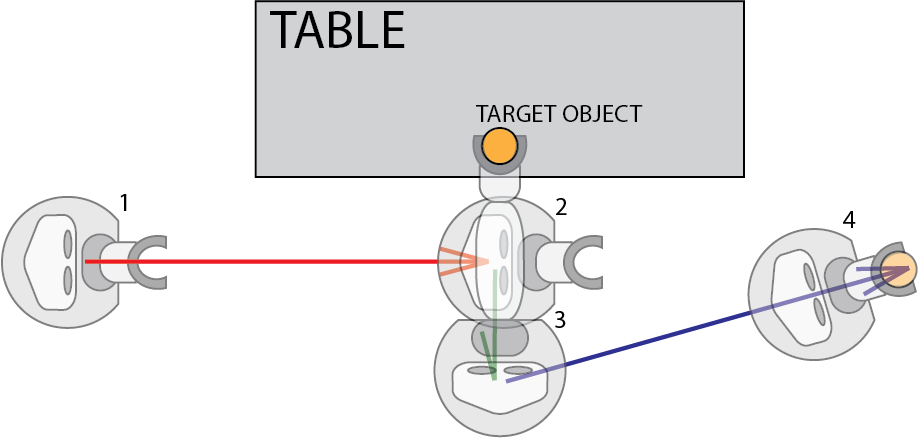
\includegraphics[width=0.45\linewidth]{illustrator/non_driveby_white_bg.png}
            \label{fig:not_driveby}}
            \quad
            \subfigure[Proposed drive-by pick-and-place]{%
            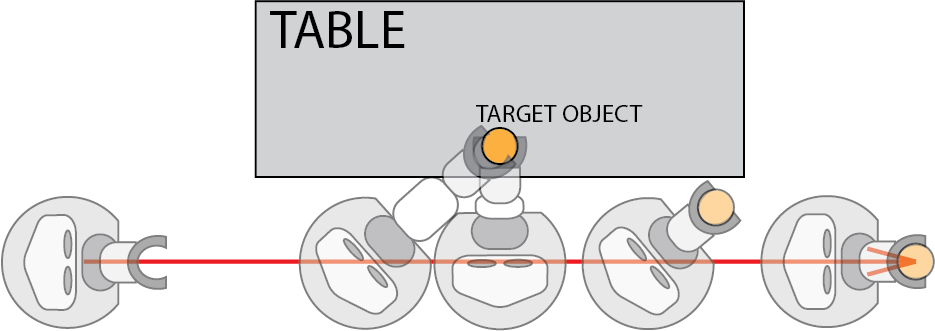
\includegraphics[width=0.45\linewidth]{illustrator/driveby_white_bg.png}
            \label{fig:driveby}}
            \caption{Depiction of pick-and-place methods}
            \label{fig:driveby_methods}
        \end{figure}

    
    \subsection{Definition and Notations}
        \iffalse Reference Steven LaValle's Book \fi
        \subsubsection{Joint Types}
            \begin{figure}[ht]
                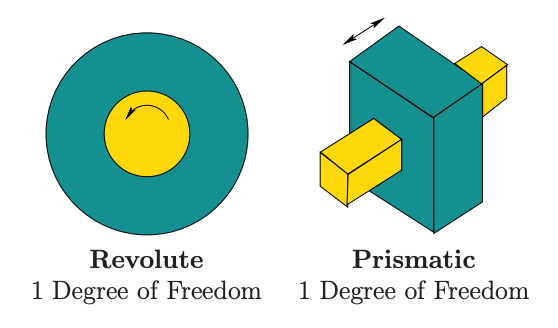
\includegraphics[width=\linewidth]{screenshots/LaValle_joints}
                \centering
                \caption{Types of joints. A continuous joint acts as a revolute joint without angle limits. From \cite{lavalle_planning_2006}, pg. 105}
                \label{fig:joints_image}
            \end{figure}
            Robot joints fall into a few distinct classes. The HSR has 3 main types of joints: continuous, prismatic, and revolute. The continuous joints include the wheels of the base, which have one rotational degree of freedom and can rotate without a limit on the angle. The HSR has prismatic joints that lift the arm and the torso. A prismatic joint has one linear degree of freedom and allows for extension and retraction. The majority of the HSR's joints are revolute joints. Revolute joints allow for one degree of rotational freedom, but have limits on allowable joint angles.\cite{lavalle_planning_2006} \cref{fig:joints_image}
        \subsubsection{Task and Configuration Space}
            Path planning for mobile robots occurs in both task space ($\mathcal{T}$) and configuration space ($\mathcal{C}$). Task space represents the set of all possible translations and rotations for the robot and its components in Euclidean space. For real robots, $\mathcal{T}\subset SE(2)$ or $\mathcal{T}\subset SE(3)$, depending on whether or not the robot's motion is confined to a plane. SE(n) denotes the Special Euclidean group, which includes any combination of translations and rotations in dimension n. For example, the HSR base is confined to the xy plane and so the position can be represented by $(x,y, \theta)$. The HSR gripper end-effector can move in three dimensions and has a task space representation of form $(x,y,z,\theta_{roll}, \theta_{pitch}, \theta_{yaw})$.
            \par The robot configuration $\mathbf{q}$ is represented by joint coordinates, which specify the degree or length value for each robot joint. As a result, $\mathbf{q}$ has the same number of elements as the number of degrees of freedom $(N)$ of the robot. The configuration space, $\mathcal{C}$, represents the set of all possible $\mathbf{q}$. $\mathbf{q} \in \mathcal{C} \subseteq$ $\mathbb{R}^{N}$. $\mathcal{C}$ is separated into $\mathcal{C}_{free}$ and $\mathcal{C}_{obs}$. $\mathcal{C}_{obs}$ represents the set of all robot configurations that result in collision with an obstacle in task space and $\mathcal{C}_{free}$ represents the set of all robot configurations that do not result in collision. Thus, $\mathcal{C}_{free} = \mathcal{C} \setminus \mathcal{C}_{obs}$.\cite{lavalle_planning_2006}

    \subsection{Robot Description}
        The HSR is one of the "Toyota Partner Robots" which aims to "provide life support and to assist with independent living in the home for handicapped people"\cite{noauthor_hsrb_manual_nodate}. The HSR is subdivided into 4 segments: the base, the torso, the arm, and the head. 
        \begin{figure}[ht]
            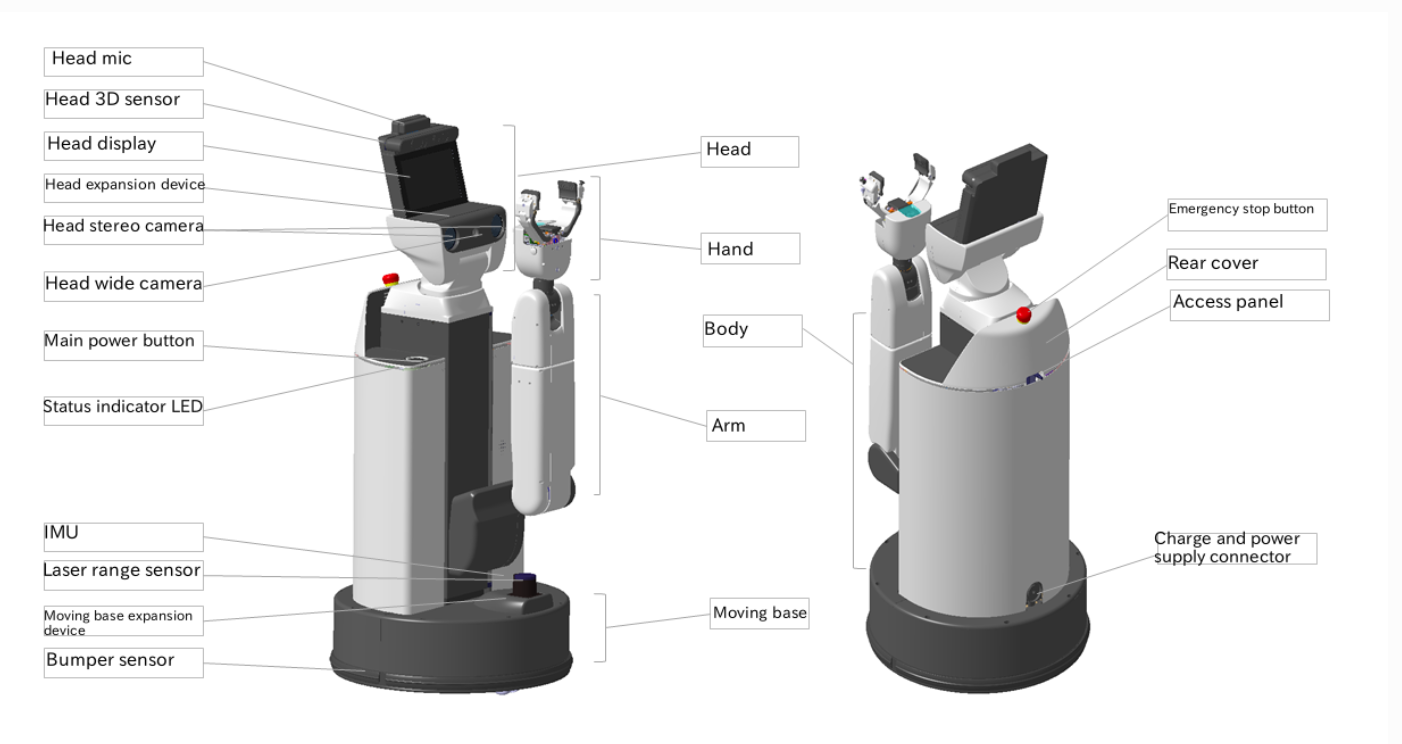
\includegraphics[width=\linewidth]{2020.05.07/hsr_overview.png}
            \centering
            \caption{Overview of HSR Segments and Components.\cite{noauthor_hsrb_manual_nodate}}
            \label{fig:hsrOverview}
        \end{figure}

        \begin{figure}[ht]
            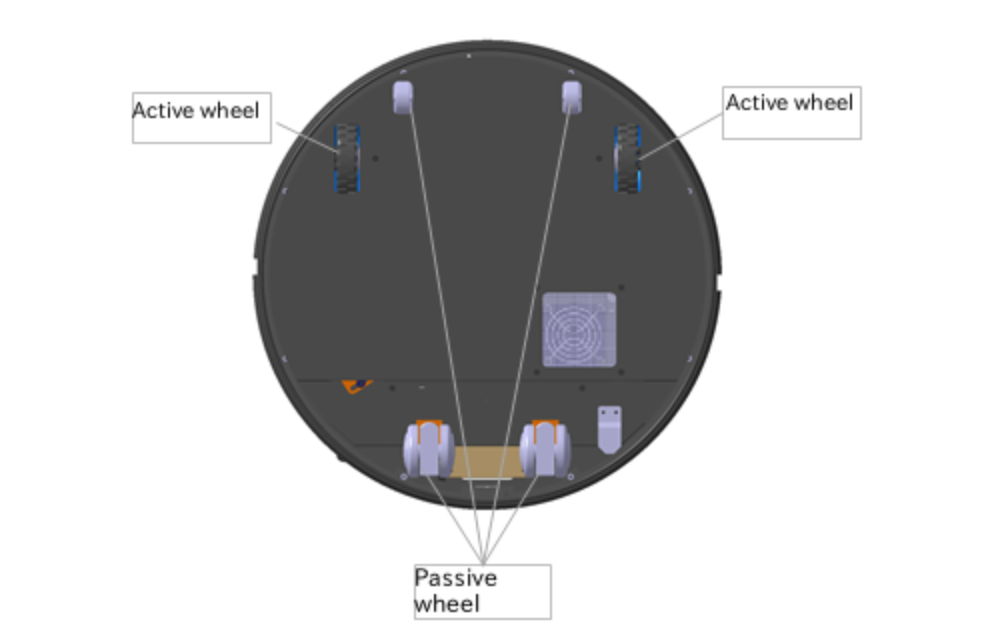
\includegraphics[width=0.60\linewidth]{2020.05.07/hsr_base.png}
            \centering
            \caption{Omnibase of HSR \cite{noauthor_hsrb_manual_nodate}}
            \label{fig:hsrBase}
        \end{figure}

        % [COMMENT] What are the advantages of an omnidirectional base? Compare and contrast with differential drive. Easier or harder? Does it imply or impose constraints?
        % [ERROR!!]
        % [COMMENT] How is it pseudo holonomic when it uses differential drive?
        % [COMMENT] [1] Clarify roll or yaw
        % [COMMENT] [2] How does it greatly aid in execution?
        \subsubsection{Base} 
            The HSR has an omnidirectional wheeled base with two rear drive wheels and two passive casters for locomotion as depicted in \cref{fig:hsrBase}. A continuous base-roll-joint \footnotemark in the HSR omnibase segment allows the body of the HSR to rotate freely of the base. The base is cylindrical and houses a bumper sensor and laser range sensor to aid in obstacle detection. A magnetic sensor allows users to mark world boundaries using strips of magnetic tape.

            \footnotetext{The coordinated for the HSR omnibase are defined such that the front of the torso points in the z-direction and the x-direction is perpendicular to the plane of the base.}
            
            \par The HSR omnibase implements a dual-wheel caster drive mechanism first described in \cite{wada_caster_2000}. The dual-wheel caster mechanism works similarly to a classical differential drive system. A differential steered robot has two separately driven wheels on either side of the robot. The robot can travel in a straight line when both wheels are driven at the same speed in the same direction. The robot turns when the wheels are driven at different speeds. The kinematics of a differential drive is,
            \begin{equation}
                \begin{bmatrix}
                    \dot{x}_{o}\\
                    \dot{y}_{o}\\
                    \dot{\theta}_{o}
                \end{bmatrix}
                =
                \begin{bmatrix}
                    r/2 & r/2\\
                    0 & 0\\
                    r/W & -r/W
                \end{bmatrix}
                \begin{bmatrix}
                    \omega_{R}\\
                    \omega_{L}
                \end{bmatrix}
            \end{equation}
            
            where $r$ is the wheel radius, $\omega_{R} and \omega_{L}$ are the angular velocities of the right and left wheel, and W is the distance between the wheels. Velocities are defined with respect to the midpoint between the wheels $(O_o)$, which coincides with the center of the robot base in a differential drive robot. This allows a differential drive robot to turn in place. The velocity in the y-direction is always zero, so a differential drive vehicle cannot move sideways. Because the local degrees of freedom of movement for a differential drive robot is less than the global degrees of freedom, differential drive robots are non-holonomic. Holonomicity is important because motion control for a holonomic robot is easier than for a non-holonomic robot.\cite{newman_c18_2017} For example, instead of having to parallel-park a car, which is a non-holonomic vehicle, a holonomic vehicle can simply drive sideways into a parallel parking space.

            \par The dual-wheel caster mechanism removes the holonomic constraint in the y-direction by offsetting the midpoint between the driven wheels and the center of the rotational stage by a distance $s$ as shown in \cref{fig:dw_caster_coords}. The rotational stage is analogous to the body of the HSR which rests on top of the base-roll-joint. This is depicted as the base-link frame in \cref{fig:base_roll_fig}. This offset results in the same kinematics as differential drive with respect to $O_{o}$. However, the kinematics with respect to the center of the rotational stage becomes,
            \begin{equation}
                \begin{bmatrix}
                    \dot{x}_{d}\\
                    \dot{y}_{d}\\
                    \dot{\theta}_{d}
                \end{bmatrix}
                =
                \begin{bmatrix}
                    1 & 0 & 0\\
                    0 & 1 & S\\
                    0 & 0 & 1
                \end{bmatrix}
                \begin{bmatrix}
                    \dot{x}_{o}\\
                    \dot{y}_{o}\\
                    \dot{\theta}_{o}
                \end{bmatrix}
                =
                \begin{bmatrix}
                    r/2 & r/2\\
                    rs/W & -rs/W\\
                    r/W & -r/W
                \end{bmatrix}
                \begin{bmatrix}
                    \omega_{R}\\
                    \omega_{L}
                \end{bmatrix}
            \end{equation}

            The shift in wheel placement results in a robot that has a non-zero velocity in the y-direction when turning. The dual-wheel caster drive mechanism resolves the non-holonomic constraint of differential drive-by forgoing the ability to turn in place. The omnidirectional base allows the HSR to take a direct path to a goal point, which simplifies paths.

            \begin{figure}[ht]
                \centering
                \subfigure[Dual-wheel caster mechanism]{%
                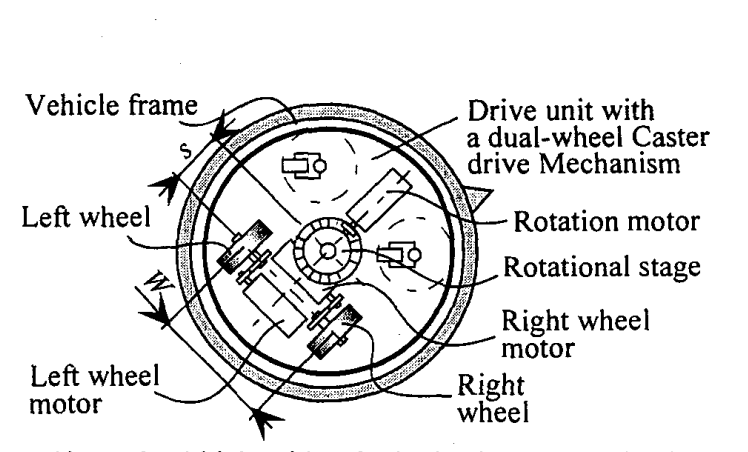
\includegraphics[width=0.52\linewidth]{screenshots/dw_caster}
                \label{fig:dw_caster}}
                \quad
                \subfigure[Coordinate system of the vehicle]{%
                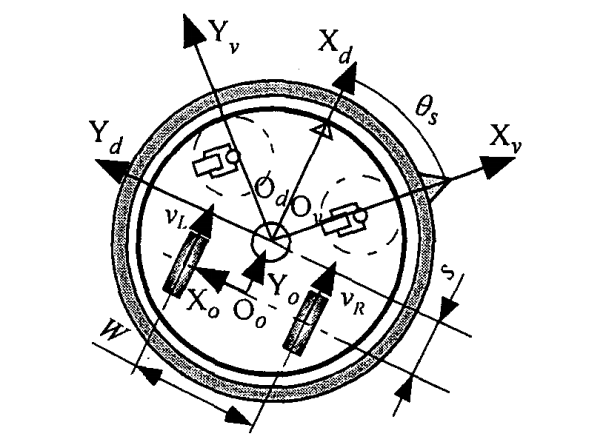
\includegraphics[width=0.38\linewidth]{screenshots/dw_caster_coord}
                \label{fig:dw_caster_coords}}
                \caption{Visualizations for dual-wheel caster mechanism from \cite{wada_caster_2000}.}
                \label{fig:dwc}
            \end{figure}
            \iffalse
            [The omnibase of the HSR uses differential steering to turn and move forwards and backwards.][Need to go through: A mobile platform with a dual-wheel caster-drive mechanism for holonomic and omnidirectional mobile robots reference. similar to differential drive but some key differences. They somehow claim holonomicity. paper is in japanese though.] A continuous base \iffalse [1] roll joint \fi in the HSR omnibase segment allows the body of the HSR to rotate freely of the base \cref{fig:base_roll_fig}. This feature \iffalse [2] greatly aids \fi in the execution of a drive-by pick-and-place trajectory. \fi

            % [COMMENT]: base roll link or yaw?
            \begin{figure}[ht]
                \centering
                \subfigure[]{%
                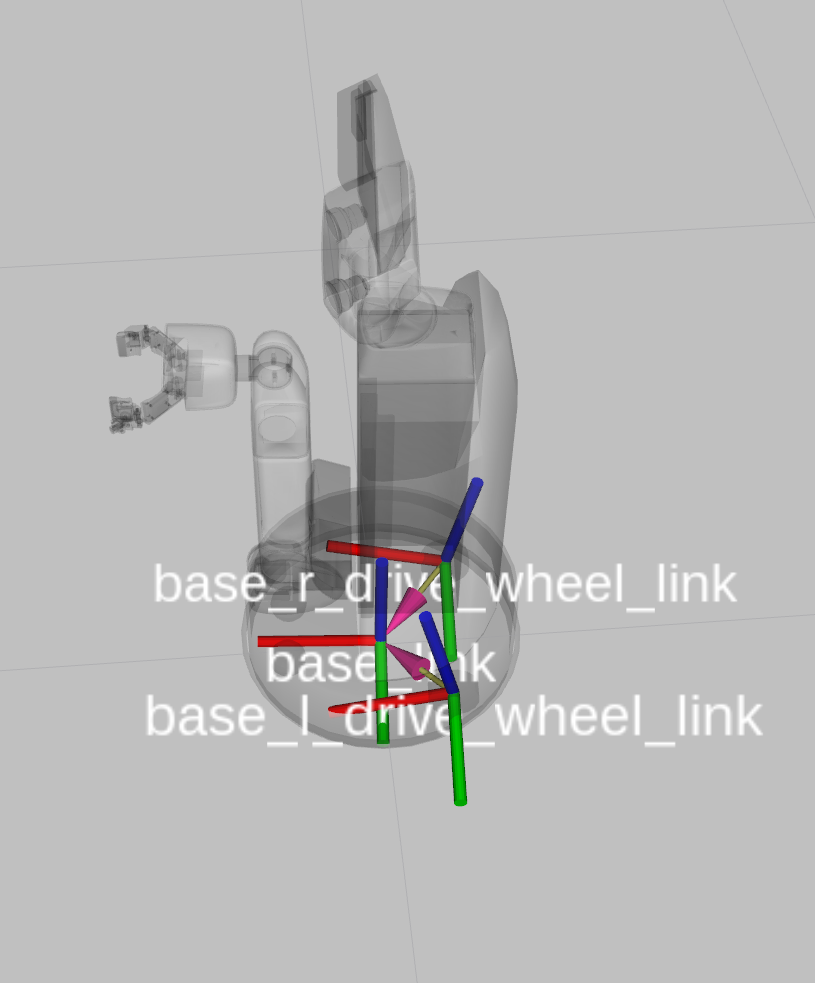
\includegraphics[width=0.45\linewidth]{2020.05.07/base_roll_0_cropped.png}
                \label{fig:base_roll_0}}
                \quad
                \subfigure[]{%
                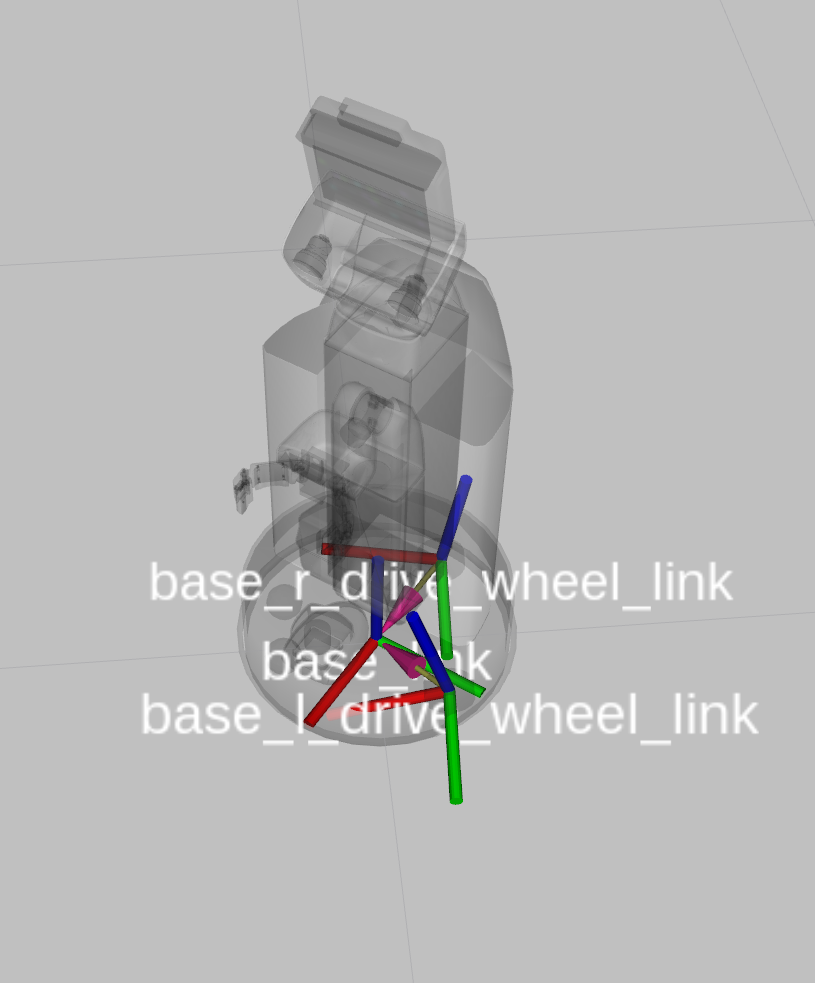
\includegraphics[width=0.45\linewidth]{2020.05.07/base_roll_1_cropped.png}
                \label{fig:base_roll_1}}
                \caption{The base roll link allows the HSR to rotate its torso without moving the omnibase. Note that the orientation of base\_link changes between (a) and (b), while the drive wheels remain stationary.}
                \label{fig:base_roll_fig}
            \end{figure}
        
        % [ERROR]
        % [COMMENT]: [1] XTion is 2.5D sensor, even though it is used for 3D perception.
    
        \subsubsection{Body and Head} 
            The HSR has a height range between 1.0m and 1.3m due to a telescoping body. The head contains a wide angle camera, stereoscopic camera, and an \iffalse [1] three-dimensional \fi ASUS Xtion depth sensor for visual input and object recognition. In addition, there is a microphone and screen display for human input. The head can pan and tilt.
        \subsubsection{Arm and Hand}
            The arm is attached to the body by a lifting shoulder joint that vertically telescopes the head and arm. The arm, including the lift joint, has 5 degrees of freedom and a length of 0.60 meters. The end effector is a two-finger rubber gripper (hand) with a camera, force sensor, and suction pad. The gripper can open to a maximum of 13.5cm, apply a maximum of 40N of force, and open and close within 0.4 seconds.
            \iffalse
            \begin{figure}[ht][ht]
                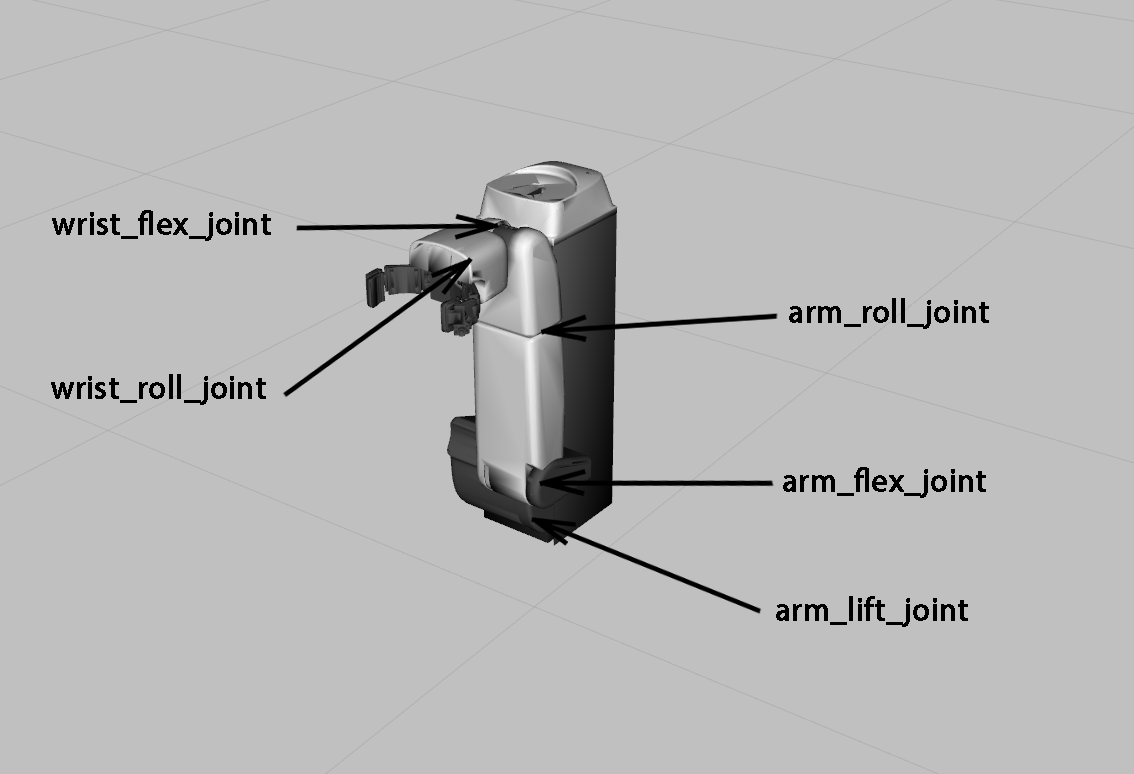
\includegraphics[width=0.60\linewidth]{2020.05.07/Arm_labeled.png}
                \centering
                \caption{HSR arm joints}
                \label{fig:armLabels}
            \end{figure}
            \fi
            % image of arm joints
            \begin{figure}[ht]
                \centering
                \subfigure[arm-lift-joint]{%
                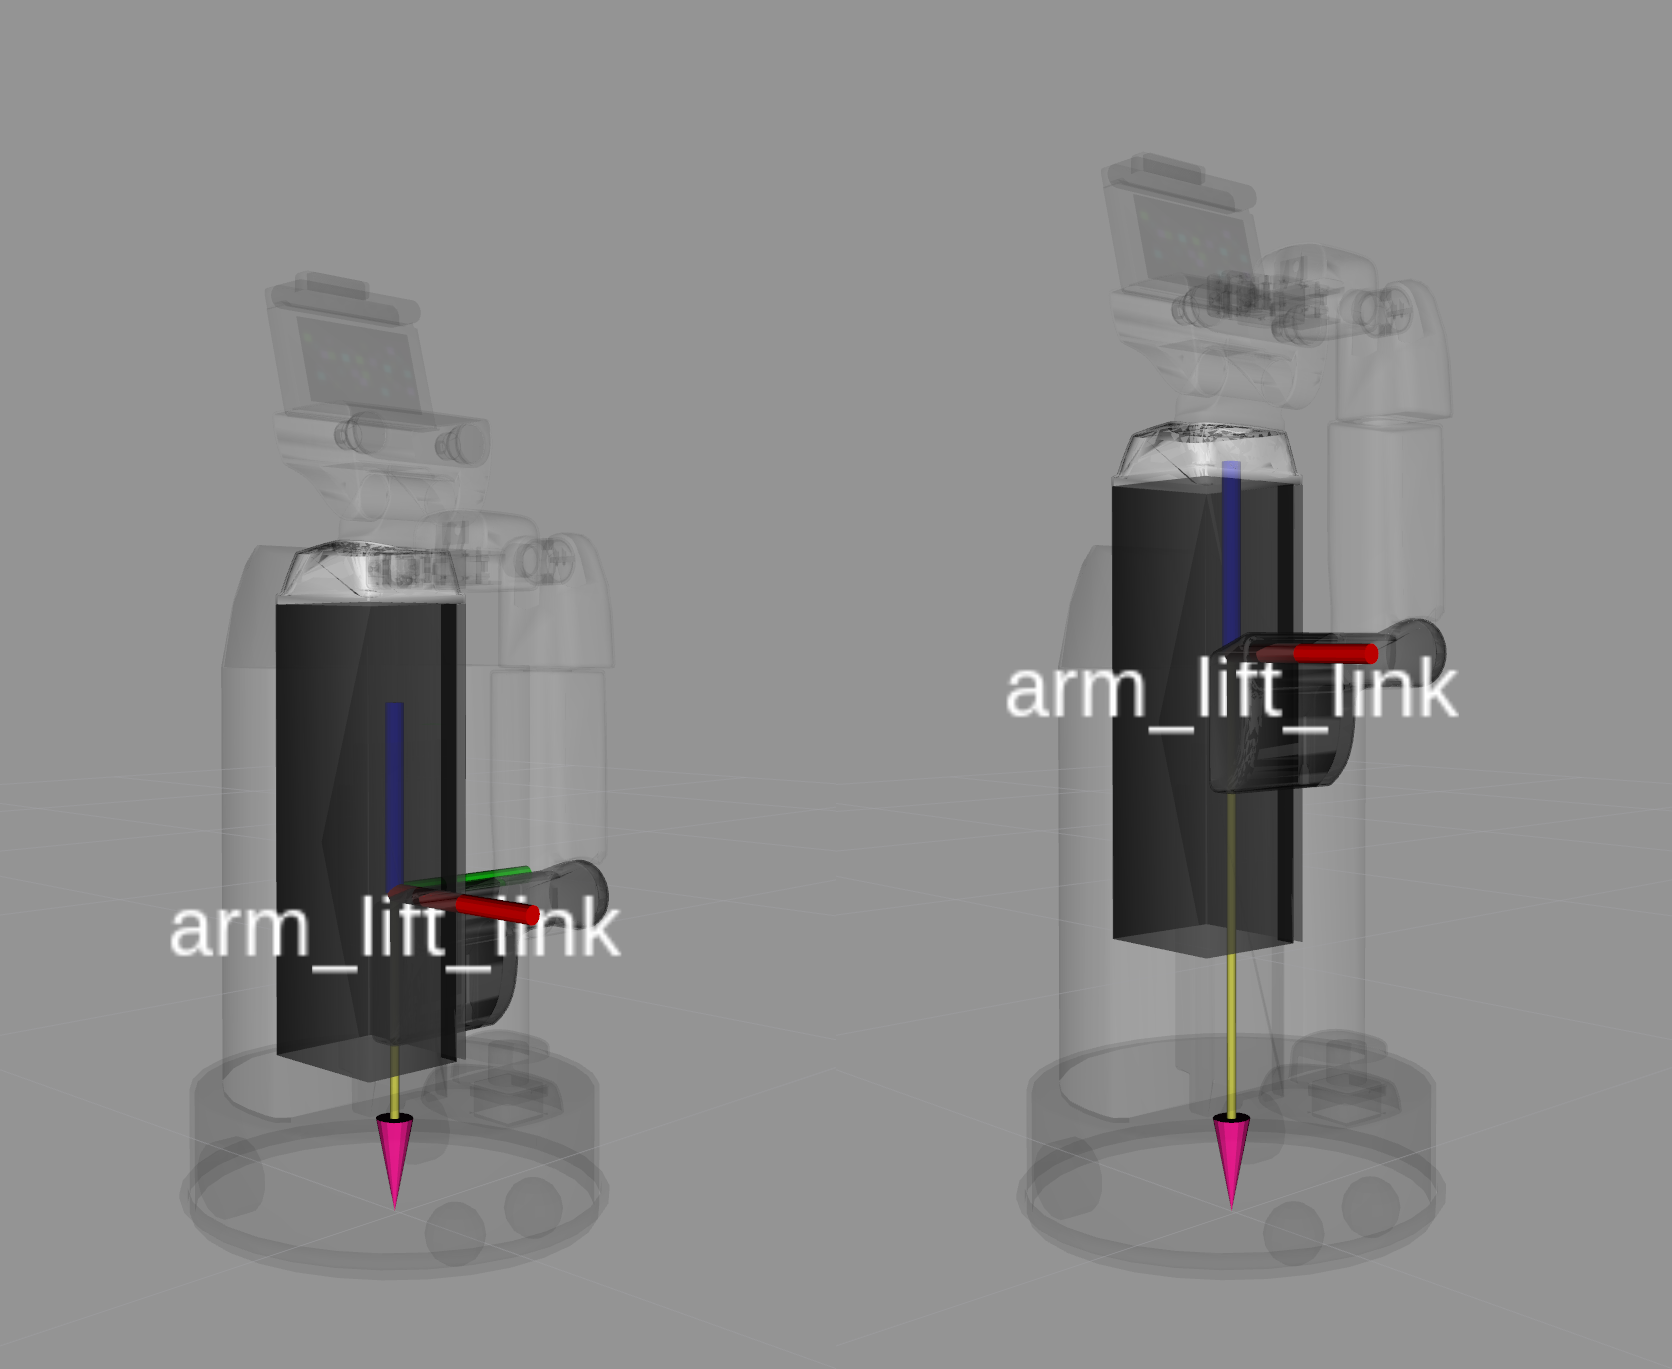
\includegraphics[width=0.3\linewidth]{joints/d_arm_lift.png}
                \label{fig:arm-lift-joint}}
                \quad
                \centering
                \subfigure[arm-flex-joint]{%
                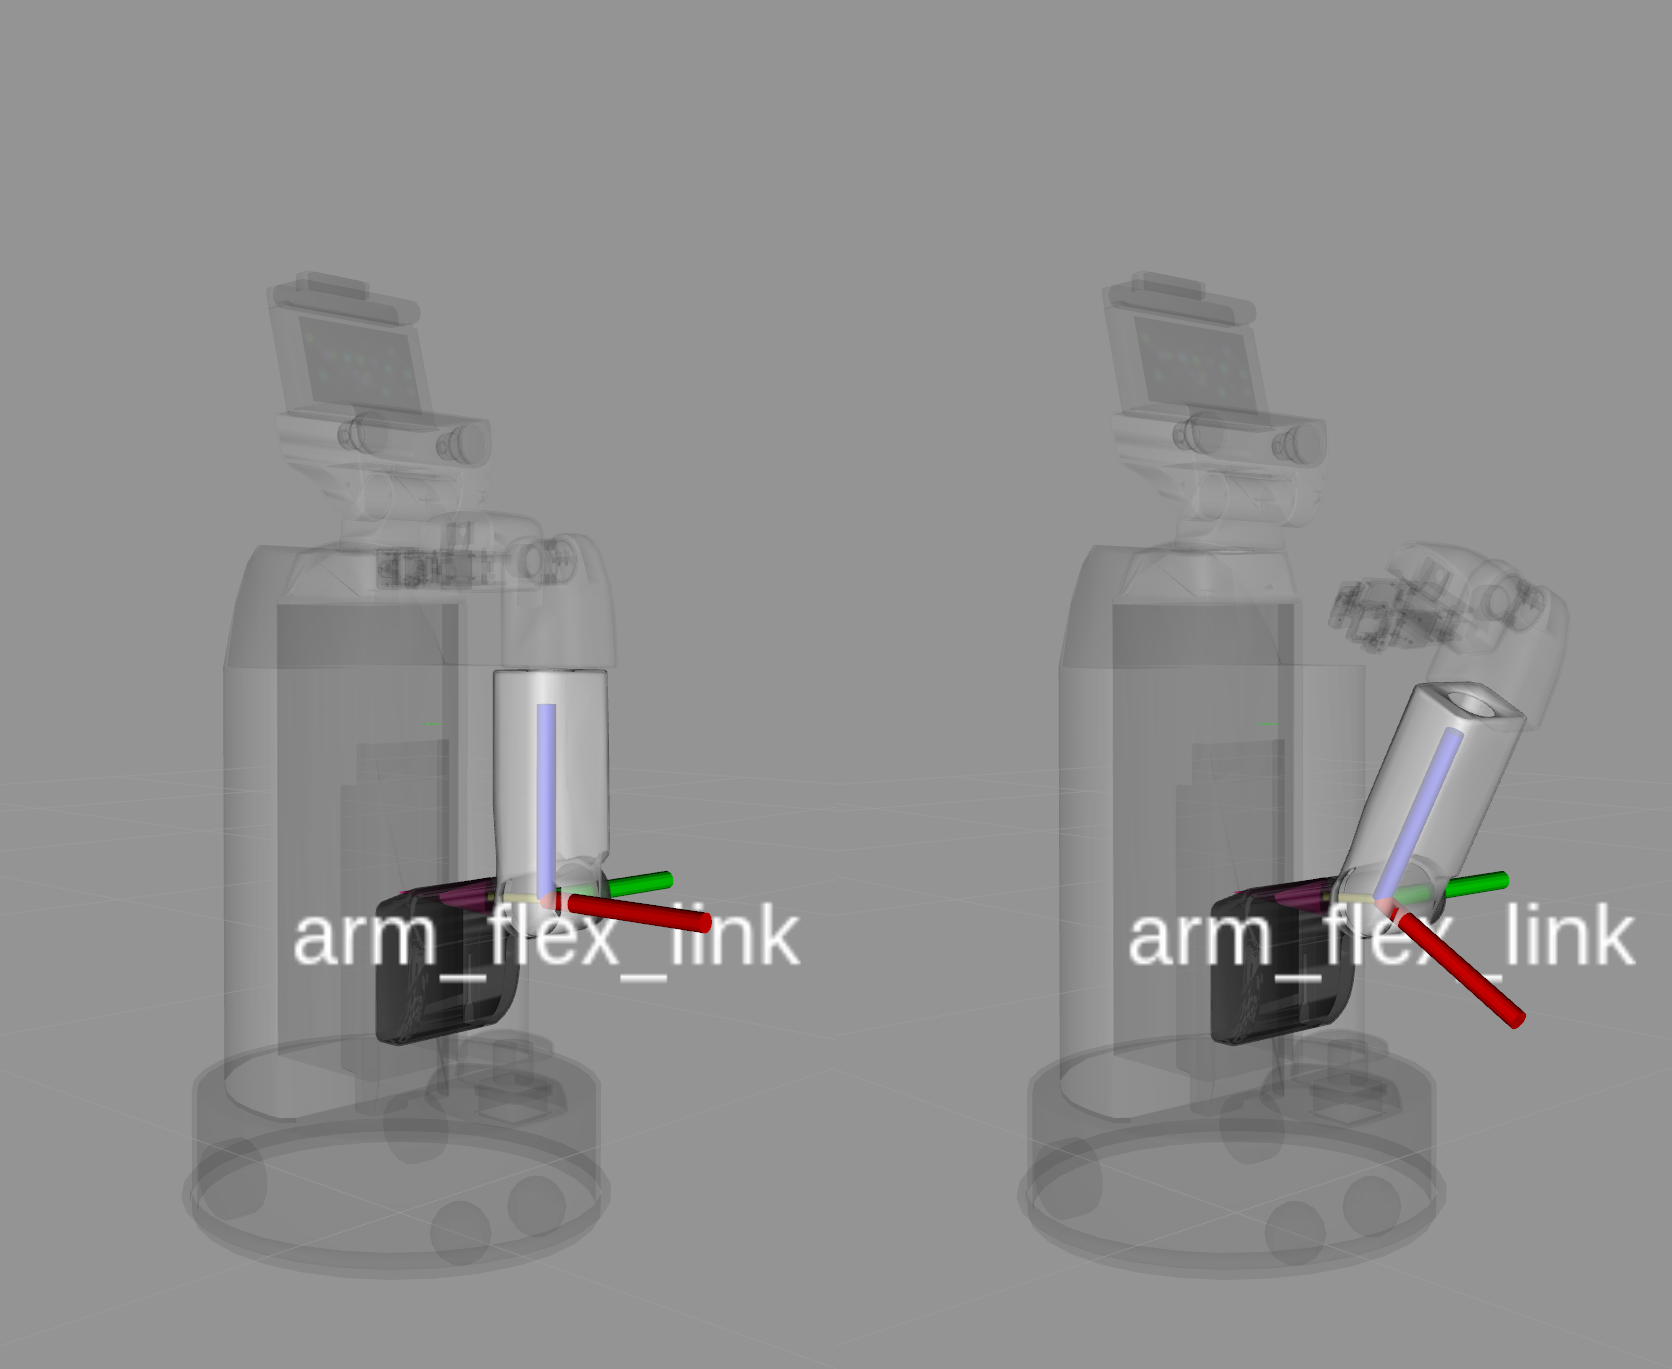
\includegraphics[width=0.3\linewidth]{joints/d_arm_flex.png}
                \label{fig:arm-flex-joint}}
                \quad
                \centering
                \subfigure[arm-roll-joint]{%
                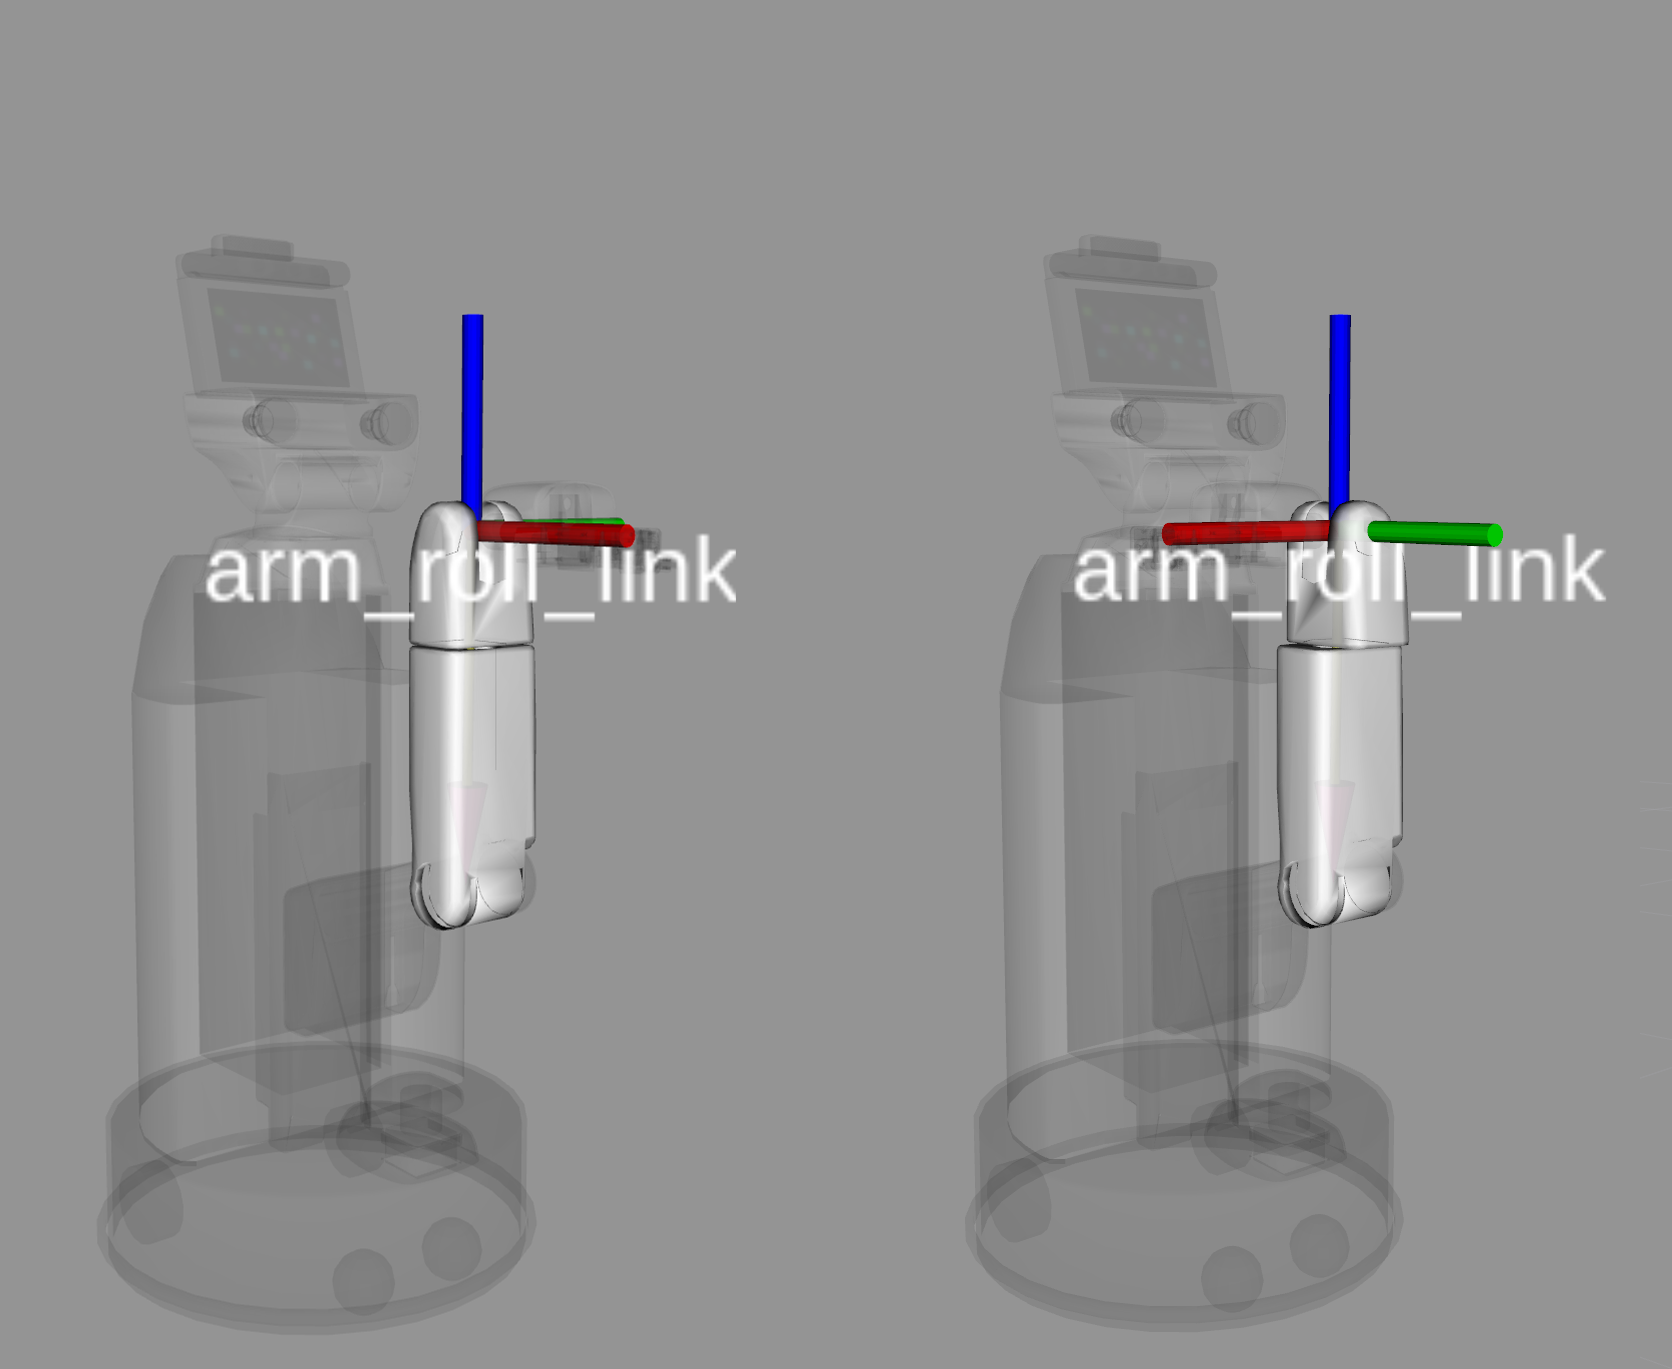
\includegraphics[width=0.3\linewidth]{joints/d_arm_roll.png}
                \label{fig:arm-roll-joint}}
                \quad
                \centering
                \subfigure[wrist-flex-joint]{%
                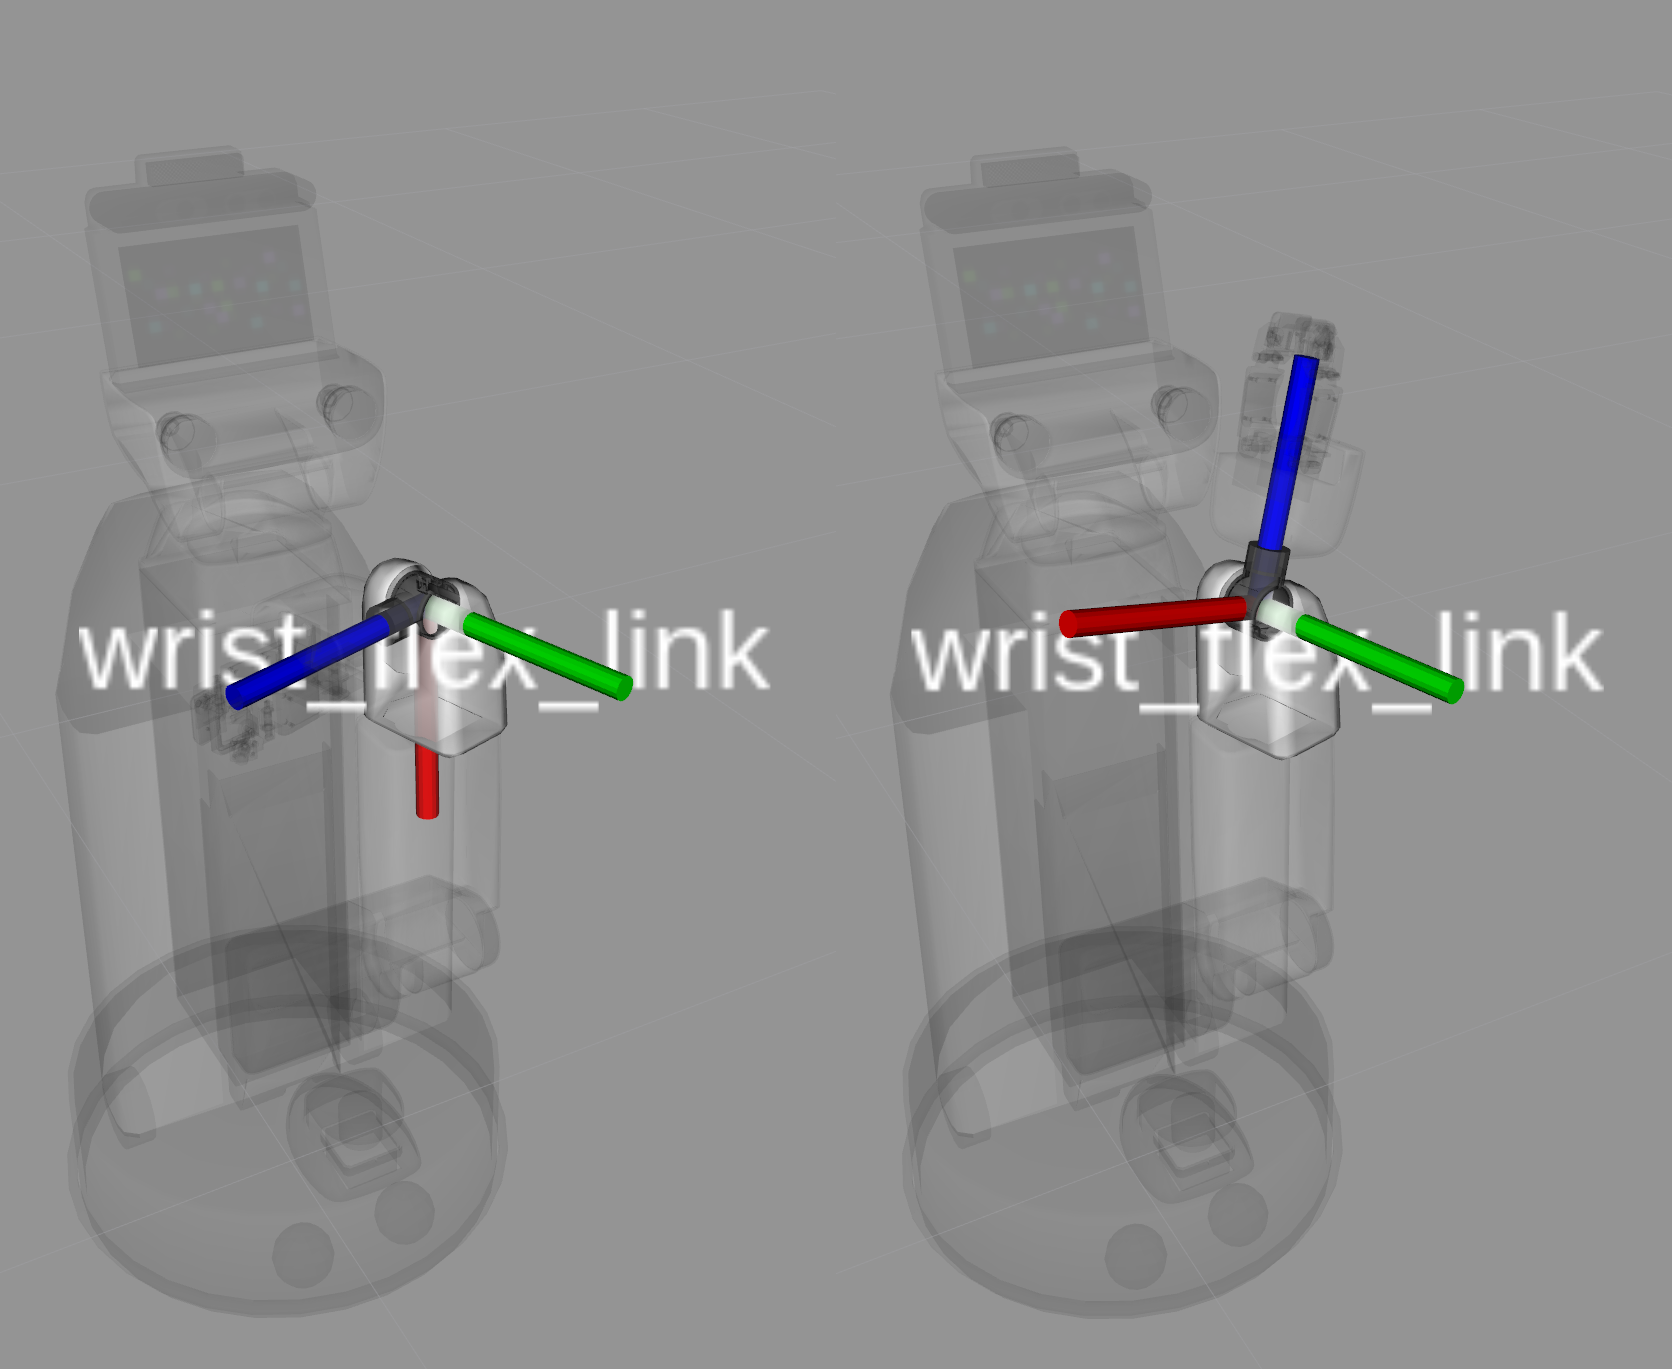
\includegraphics[width=0.3\linewidth]{joints/d_wrist_flex.png}
                \label{fig:wrist-flex-joint}}
                \quad
                \centering
                \subfigure[wrist-roll-joint]{%
                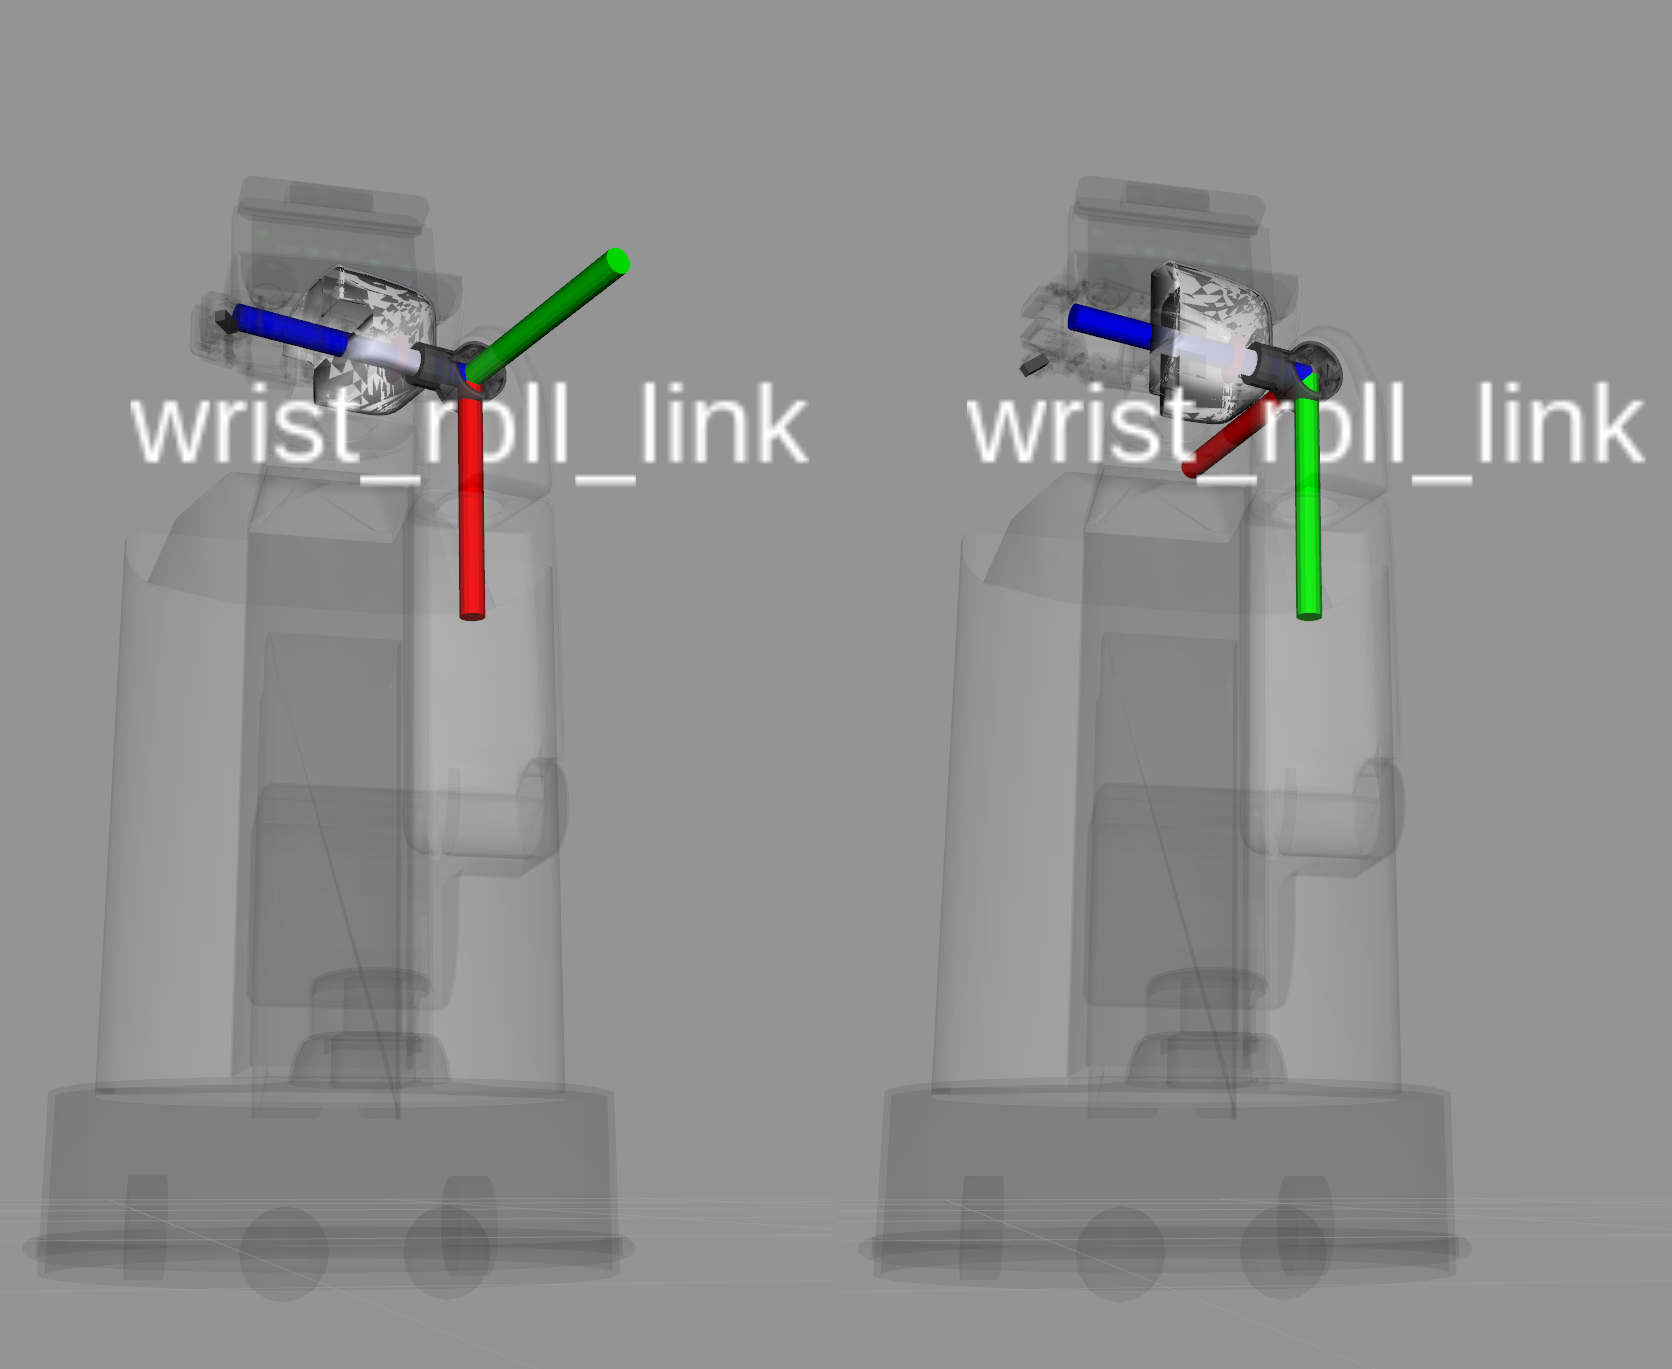
\includegraphics[width=0.3\linewidth]{joints/d_wrist_roll.png}
                \label{fig:wrist-roll-joint}}
                \quad
                \caption{HSR arm joints}
                \label{fig:HSR-joints}
            \end{figure}
        \subsubsection{Development}    
            The HSR has software built on top of the Robot Operating System (ROS), which is an open-source framework used to write robot software.\cite{quigley_ros_2009}. The HSR software includes a Python Interface and ROS interface. Toyota introduces an interactive shell based on iPython as an option for users to interface with the HSR without the steep learning curve associated with ROS. This shell interface allows for whole body motion, as well as individual subsystems by specifiying goal points, goal poses, and relative movement. Further, the HSR has a graphical web-interface for usage by non-technical operators that allows for basic teleoperation.
    % \subsection{Proposed Solution}
    %     [move to technical]
    %     The solution to the drive-by pick-and-place problem closely follows the method outlined in (Time series ***). The paper details a solution where a pick-and-place problem is split into 3 parts: reaching, pick-and-place, and a second reaching phase. However, due to issues of reachability resulting from the joint position limits of the HSR, a simplified approach was taken where the entire pick-and-place trajectory is solved using the method in the picking segment. <go into pick and place literature>.
    % \subsection{Time series ***}
    \newpage
\section{Planning Algorithms}
    % [COMMENT][ERROR] Navigation: path planner rather than motion planner. Do I want to speak on something else than navigation here?
    % [COMMENT][ERROR] later I mention that motion planning modification will be made -for navigation? Or whole-body planning? If so: I need to introduce what the difference between the things are, and why say whole-body is rare in practice (keyword: locomanipulation)
    % [COMMENT][CRITICAL*] What is motion planning? Why is it needed? What are the classes? Are RRT and AICO in the same class? Why would you use one over the other?
    \subsection{Overview}
    \iffalse
        % Navigation for autonomous mobile robots relies on two primary systems: a robot state estimator and a path planner\iffalse motion planner \fi. The base HSR has implementations of both systems. For the purpose of accomplishing a drive-by pick-and-place task, modifications will be made to the motion planning algorithm. The motion planning algorithm utilized in this project concatenates paths planned using Rapidly-Exploring Random trees and a non-linear programming solver called Approximate Inference Control (AICO).
    \fi
        To perform a drive-by pick-and-place task, the HSR must satisfy constraints such as avoiding self-collision, avoiding collision with obstacles, and maintaining a given base trajectory. This is a whole-body locomanipulation task, which is defined as actions that involve the whole body of a robot for locomotion, manipulation, or stabilization.\cite{kaiser_validation_2015}. Since the HSR is a wheeled-base robot, stability is not as large of a concern compared to legged, walking robots, for which whole-body loco-manipulation planning is mainly used. HSR joint limits prevent the robot from falling over and the maximum recommended weight of objects is 500g, much greater than the soda can be used in testing.\cite{noauthor_hsrb_manual_nodate} In addition to considering multiple constraints, whole-body motion planning poses the difficulty of planning motion for a large number of degrees of freedom. However, whole-body motion planning allows the robot to simultaneously drive-by and pick up an object as in \cref{fig:driveby}.
        \par Planning the path of the HSR base and end-effector is performed by a path planner. In this project, two classes of planners are used: sampling-based planners and trajectory optimization planners. Sampling-based approaches randomly sample the free configuration space to identify collision-free paths between a start and goal state. Optimization-based planners minimize an objective function composed of smoothly differentiable constraints to produce a collision-free and smooth trajectory. Implementations of both types of planners will be described and compared to justify their usage.
    
    % [COMMENT]: [1] how/with what mechanism?
    % [COMMENT]: [2] Maybe move to section 5.1
    % \subsection{Rapidly-Exploring Random Trees}
    \subsection{Sampling-Based Planning}
        Two common sampling-based planners are Probabilistic Roadmaps (PRM) and Rapidly Exploring Random Trees(RRT). Both methods are probabilistically complete, meaning that if a solution exists, it will be discovered given infinite time. A variation of the RRT algorithm is used in this project. A description of PRM is included since LaValle closely compares RRT to PRM in the original RRT paper, and thus it serves as a good starting point for sampling-based planning.\cite{lavalle_rapidly-exploring_1998}
        % Rapidly-Exploring Random Tree algorithm (RRT) and its variants are widely used for autonomous path planning for mobile robots. Proposed by Steven LaValle in 1998, RRT is a sampling-based planning method that is probabilistically complete and [1] naturally accommodates non-holonomic constraints. 
        
        % \iffalse RRT builds on the Probabilistic Roadmap planning method, which has the desirable property of being probabilistically complete but lacks the ease of extension to non-holonomic systems. \fi
        % \par Sampling-based planners are designed to adeptly search high dimensional configuration spaces without the high computation power required for dynamic programming [Bellman, 1957]. \iffalse Due to the probabilistic completeness that arises from the process of randomly sampling configurations,  sampling-based planners can also better avoid the issue of becoming trapped in a local minima as in the case of gradient-descent approaches.\fi

        % [COMMENT] [CLARIFY]: Why is PRM under the RRT section? What is the relation?
        \subsubsection{PRM}
            \begin{figure}[ht]
                \subfigure[PRM Algorithm \cite{kavraki_probabilistic_1996}]{
                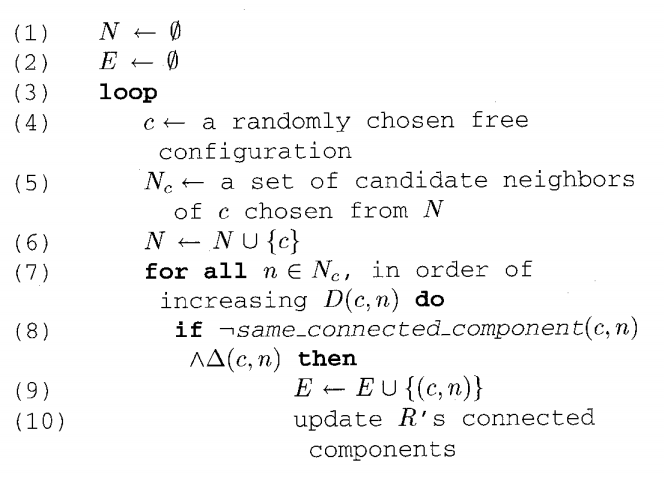
\includegraphics[width=0.45\linewidth]{images/algorithms/prm.png}
                \centering
                \label{fig:prm_algo}}
                \quad
                \subfigure[Example of PRM \cite{gammell_c18_nodate}]{
                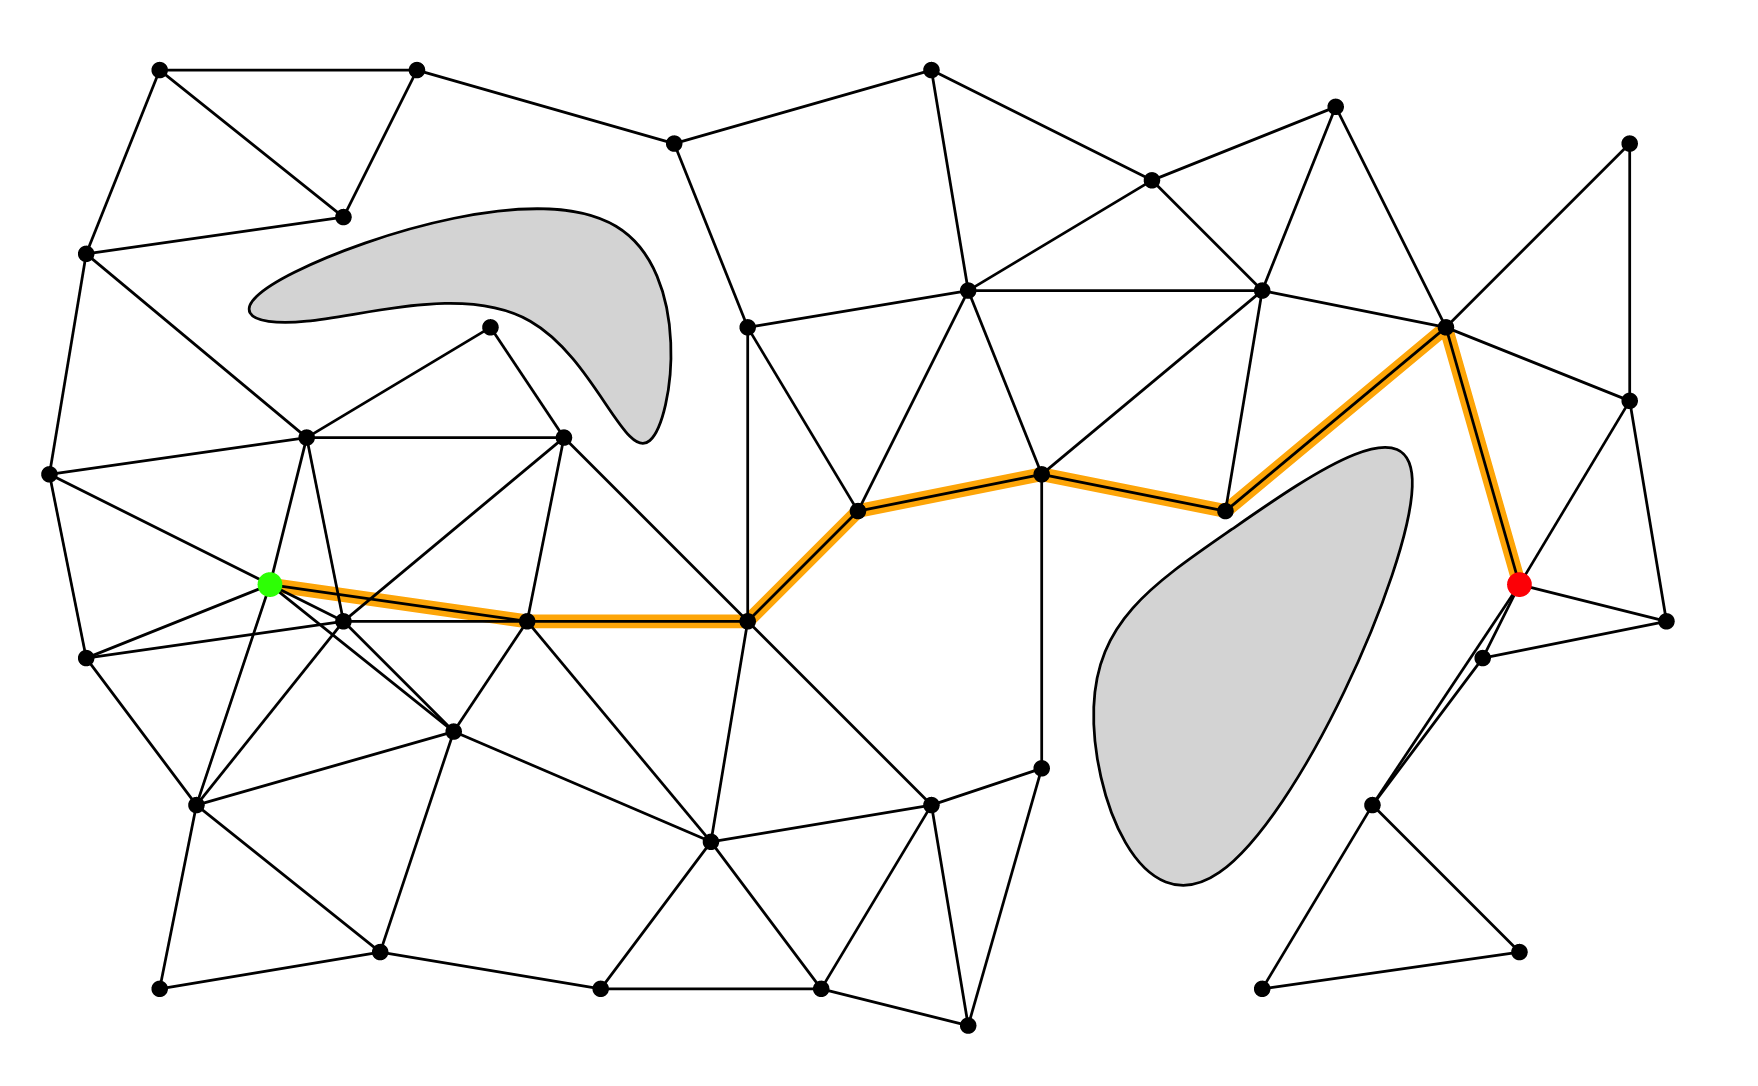
\includegraphics[width=0.45\linewidth]{images/algorithms/prm_image.png}
                \centering
                \label{fig:prm_image}}
                \caption{Probabilistic Roadmap}
                \label{fig:prm}
            \end{figure}

            A PRM is initialized with the starting state of the robot and a desired goal state. Robot configurations are randomly drawn from the set of free configurations. This implies that a map of the environment with obstacles and free regions is known. These random configurations are represented as nodes on a graph. Neighboring nodes with an unobstructed path and a distance below a given threshold are connected. This represents a valid path between two configurations. An issue arises here as a euclidean distance metric gives a computational speed advantage, but assumes holonomicity. Alternatively, [PRM paper] proposes using a local planner to calculate swept-area/volume as a distance metric, which would allow the method to extend to non-holonomic robots, but the authors note that this method is time-consuming. Given sufficient samples, the nodes would fill the entire free configuration space. A unidirectional search of the network using an algorithm like Dijkstra's shortest path would give the shortest valid path in the PRM. Given infinite random samples, the PRM method would search the entire free configuration space, meaning that it is asymptotically optimal \cite{newman_c18_2017}. Further, since the random sampling is not affected by the start and end states, the roadmap can be saved and queried for other start and end states, reducing computation time for subsequent planning calls. This property makes PRMs a multi-query planner, since multiple plans vith varying start and goal states can be generated from a single roadmap. 
            \par The drive-by pick-and-place method does not require many paths to be planned, so the exhaustive planning in configuration space provided by a PRM is not necessary. This motivates the need for single-query planners that can more efficiently identify a single valid path. Such an example is the RRT planner.
            % \par The main issue with PRM is that for every new sample, a k-nearest-neighbor query is performed to identify neighobring nodes within a threshold distance. This computation becomes increasingly expensive as the number of nodes in the PRM increases. 
        \subsubsection{Vanilla RRT}
        \begin{figure}[ht]
            \subfigure[RRT Algorithm \cite{lavalle_rapidly-exploring_1998}]{
            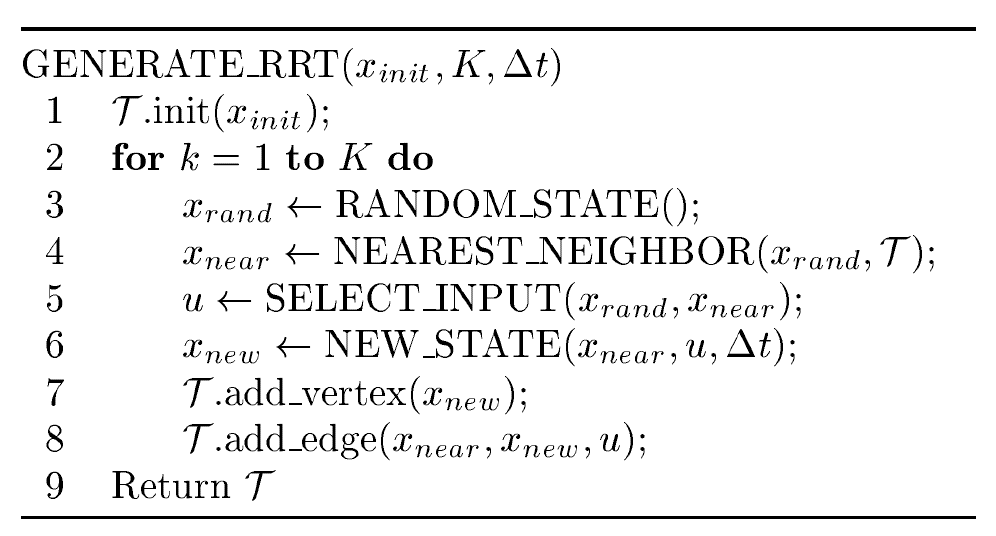
\includegraphics[width=0.45\linewidth]{images/algorithms/rrt.png}
            \centering
            \label{fig:rrt_algo}}
            \quad
            \subfigure[Example of RRT \cite{gammell_c18_nodate}]{
            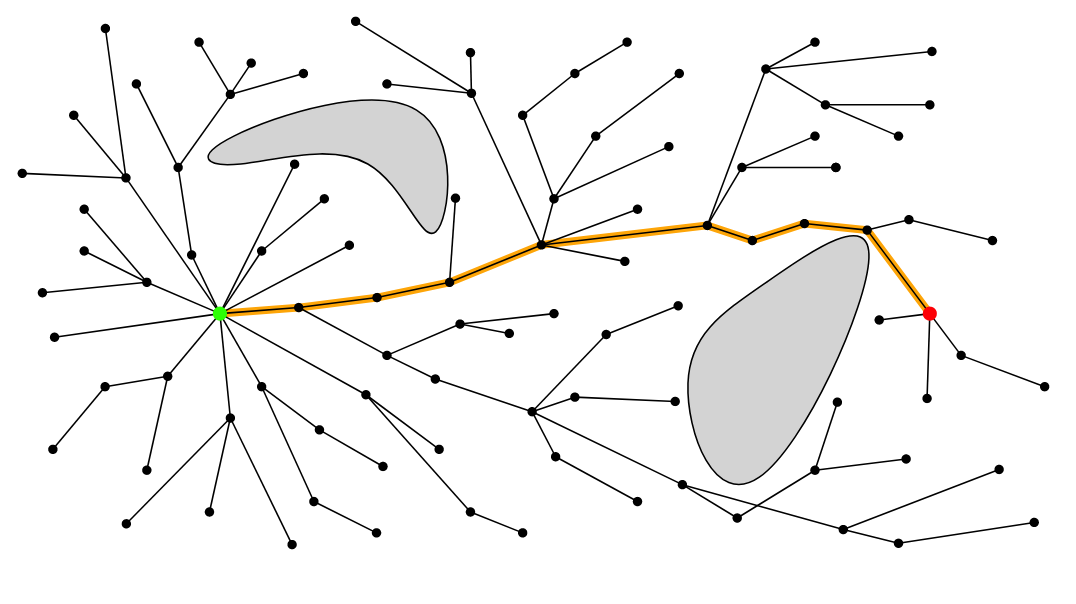
\includegraphics[width=0.45\linewidth]{images/algorithms/rrt_image.png}
            \centering
            \label{fig:rrt_image}}
            \caption{Rapidly-Exploring Random Trees. (a): $x_{init}$ is the start state, $K$ is the number of verticies, and $\delta t$ is a time interval. Note, the algorithm in (a) simply explores the free configuration space.}
            \label{fig:rrt}
        \end{figure}
            % touch on single and multi-query.
            \par \iffalse As mentioned previously, RRT builds on the PRM method.\fi Rapidly-Exploring Random Tree algorithm (RRT) and its variants are widely used for autonomous path planning for mobile robots. Proposed by Steven LaValle in 1998, RRT is a sampling-based planning method that is probabilistically complete and [1] naturally accommodates non-holonomic constraints. Instead of creating a cyclic graph in the case of the PRM, RRT forms an acyclic, directed tree rooted at the starting configuration node. Like PRM, RRT is also a sampling-based planner, although when extending the graph, a randomly generated configuration is not directly added to the tree. Instead, as the name suggests, Rapidly Exploring Random Trees take a step in a random direction to explore the free configuration space. A step of a given length is taken towards the random configuration from the closest node of the tree, given that the step does not result in a collision with an obstacle. This gives a slight advantage over PRMs since only a single nearest neighbor query is required. Once a branch of the tree steps within a threshold distance of the goal, a path from the start configuration to the goal configurations is found. Since the graph is rooted, directed, and acyclical, the solution is easily found with a simple tree traversal. 
            \par Unlike PRM, which is a multi-query method, the tree for RRT is rooted at the starting node, so this single-query algorithm must be rerun for differing start and end states. RRT maintains probabilistic completeness for holonomic systems due to the random sampling of the free configuration space, given that states are uniformly sampled. LaValle explains the probabilistic completeness property in terms of a Voronoi diagram of RRT vertices. Due to random sampling, exploration is biased towards large Voronoi regions, converging to a complete, uniform (or another sampling scheme) search of the free configuration space as large Voronoi regions are iteratively reduced. [image of voronoi] RRT also more readily adapts to non-holonomic constraints compared to PRMs. This is due to the directed nature of the tree. The closest node to a random configuration can be determined by a metric that accounts for a constraint such as rotation. The path from the closest node to the new node can be found by inverse kinematics under non-holonomic constraints.
        \subsubsection{Bidirectional RRT Variants}
            RRT has numerous variants, notably Optimal RRT (RRT\(^*\)) which reorganized the tree structure as new nodes are generated. Two variants relevant to this project are RRT-Connect and Constrained BIDirectional RRT (CBiRRT2). A time-series RRT Connect algorithm is implemented in [Time Series Planning ***] which is detailed in [Section Reference]. The HSR utilizes a planner that builds upon CBiRRT2. Both RRT-Connect and CBiRRT2 are bi-directional RRT variants, meaning that trees are extended from both the start and goal nodes by swapping the start and goal trees each loop. RRT-Connect incorporates a Connect heuristic, which is a greedy function that takes the place of the Extend step in the original RRT algorithm. Instead of taking a single step towards a target configuration, \(q\), the Connect function iteratively extends the tree towards \(q\) until either an obstacle is encountered or the configuration is reached. LaValle and Kuffner note that q can be a random configuration or the nearest neighbor of the other tree. This allows for tuning the algorithm to prioritize either exploration or connection of the two trees.
            \begin{figure}[ht]
                \subfigure[RRT-Connect Algorithm \cite{kuffner_rrt-connect_2000}]{
                    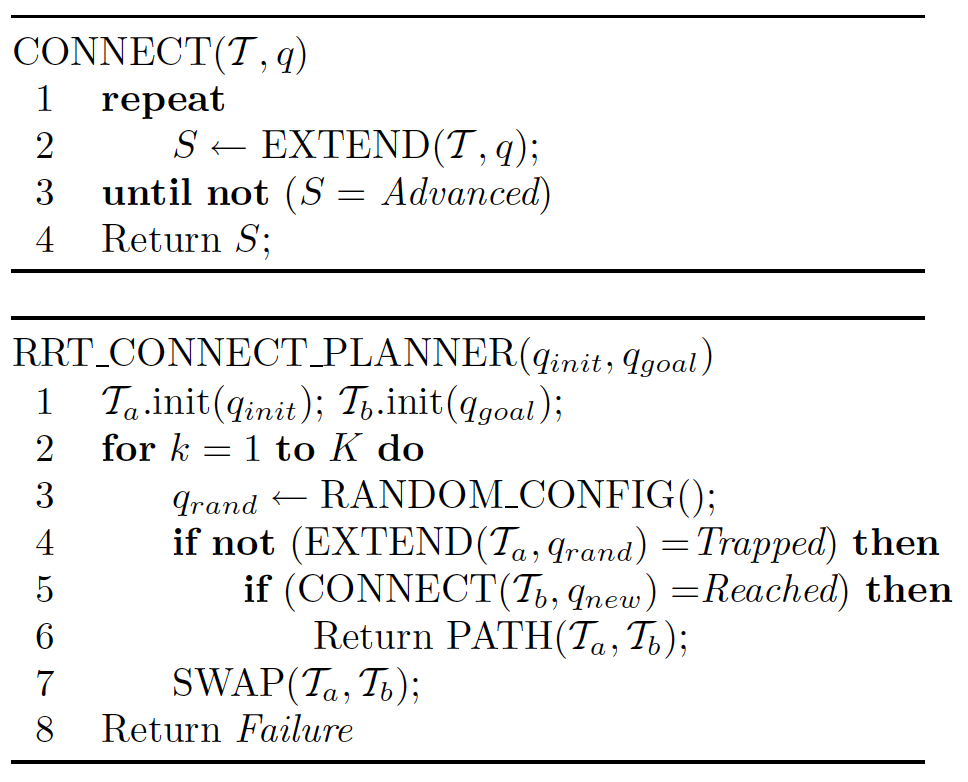
\includegraphics[width=0.45\linewidth]{images/algorithms/rrt_connect.png}
                    \centering
                    \label{fig:rrt-connect_algo}}
                \quad
                \subfigure[Example of RRT-Connect \cite{kuffner_rrt-connect_2000}]{
                    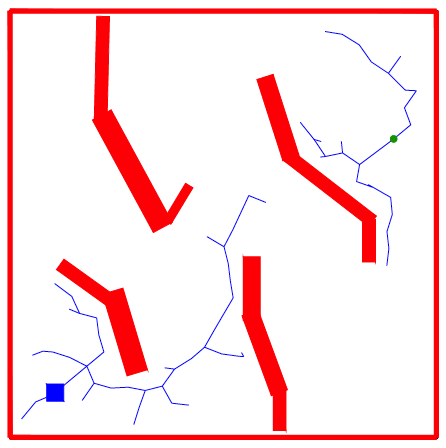
\includegraphics[width=0.45\linewidth]{images/algorithms/rrt_connect_image.png}
                    \centering
                    \label{fig:rrt-connect_image}}
                \caption{RRT-Connect}
                \label{fig:rrt-connect}
            \end{figure}

            \par The advantage of a bi-directional RRT over the original RRT is the expansion of the tree rooted at the goal node. As the goal-rooted tree expands, the number of possible points of connection increases, encompassing a larger portion of the free configuration space. This increases the rate of finding a feasible path.
            \iffalse
            % \par So far, the problems described have been confined to planning in <=3 dimensions which is intuitively understandable by humans, with a vague suggestion of application to higher dimensions. This is satisfactory to describe the planning for the omnidirectional base of the HSR, which has motion in x, y, and \(\theta\). However, in whole-body planning for the HSR with 8-dof (3-dof base + 5-dof arm), higher dimension constraint manifolds represent the possible configurations of the robot that satisfy given constraints. The goal remains the same: to find a path from start to end states in task space that lies completely on constraint manifolds in configuration space.
            \fi
            For a robot confined to motion in 2 dimensions, such as the HSR omnibase, sampling can occur in task space, by planning in $x,y, \theta$ coordinates, instead of wheel joint angles. The HSR omnibase controller contains software that converts omnibase goal positions to joint configurations using inverse kinematics. Inverse kinematics (IK) is the process of calculating joint configurations to satisfy an end-effector position in task space. Forward kinematics is the reverse process, which calculates the end-effector position in task space from a joint configuration. In general, inverse kinematics is much more difficult than forward kinematics. Since IK is the inverse of a function, the result may be no solution or infinitely many trajectories depending on the degrees of freedom of the system. \iffalse Researchers at Toyota found an analytical IK solution for 8 degrees of freedom (3 base DOF and 5 arm DOF) for positioning the end effector of the HSR. However, constraining the base trajectory \fi 
            For higher degrees of freedom, such as the 8 degrees of freedom HSR (3 base DOF and 5 arm DOF), it is easier to sample in configuration space, since forward kinematics is faster. In whole-body planning for the HSR, higher dimension constraint manifolds represent the possible configurations of the robot that satisfy given constraints. The goal remains the same: to find a path from start to end states in task space that lies completely on constraint manifolds in configuration space.


        \subsubsection{CBiRRT} 
            CBiRRT, the first published iteration of the algorithm, uses a method similar to the Connect-Heuristic that attempts to iteratively extend both trees towards a randomly sampled configuration. Unlike RRT-Connect, in higher dimensions, the constraint manifold may be of a lower dimension than the entire configuration space. This means rejection sampling, which is the uniform sampling the entire configuration space until a viable configuration is selected, does not work. Instead, a ConstrainedConfig step is introduced to project nodes onto the nearest constraint manifold, to ensure that configurations satisfy the given constraints. \cite{berenson_manipulation_2009}
        
        % set in more detail and novelty
        \subsubsection{CBiRRT2} 
            CBiRRT2 introduces spacial expressions called Task Space Regions (TSRs) which are used to efficiently search the configuration space, especially for end-effector manipulation with pose constraints. TSRs encode a frame in configuration space and a set of boundaries in the coordinate of the frame. TSRs are designed for sampling-based planners because they are easy to sample from and distance from a given configuration to a TSR can be quickly computed. Further, TSR's can be chained together to encapsulate multiple pose constraints on an end effector. In the CBiRRT2 algorithm, trees are grown in each iteration using one of two modes, explore and sample, determined by a set probability. The explore mode attempts to connect to a random configuration like in CBiRRT. The sample mode is a new feature that differs from CBiRRT. In sample mode, the algorithm samples from a set of TRS chains and adds a new goal node to the goal tree. One of the driving principles behind CBiRRT2, embodied by the sample mode, is the idea that a task can be accomplished in more than one way. By specifying a TSR for a goal, the CBiRRT algorithm attempts to both identify possible goal configurations that would fulfill a task, as well as solve for a path to a goal. The process of increasing the number of goal states essentially creates a pair of "seeded forests" that increase the rate of discovering a motion plan. \cite{berenson_pose-constrained_2009} 

        \subsubsection{HSR CBiRRT2 Variant}
            The HSR variant of CBiRRT2 simply varies the weighting of either arm motion or base motion. \cite{yamamoto_development_2019} Note that prioritizing arm movement results in accurate end-effector positioning, while prioritizing base movement permits the application of a larger force on an object. The HSR motion planner incorporates time-optimal path parameterization (TOPP)\cite{yamamoto_development_2019} to optimize the motion of the HSR in time under hardware constraints such as speed and torque limits. TOPP allows the HSR to reach goal poses at specified times as long as the time-from-start is greater than the optimal duration, by scaling the trajectory in time.

        \subsubsection{Commentary}
            The purpose of this project is to solve a drive-by pick-and-place problem. The HSR can already pick-and-place an object with its 'built-in' motion planner. This can be done by specifying the desired end-effector position to be reached to grasp the target object. The placement target can be specified by a second end effector target pose. The HSR can create TSRs of both target poses and two calls to the CBiRRT2 variant planner would result in a satisfactory solution to the simple pick-and-place problem. However, the drive-by component of the problem introduces a time-varying aspect that is not easily satisfied by the HSR planner.

            \par CBiRRT2 and by extension, the HSR motion planning algorithm, address scleronomic holonomic constraints, which are defined as 'time-invariant constraints evaluated at a given configuration of the robot' \cite{berenson_pose-constrained_2009}. In a practical application, the HSR must plan for motion in a dynamic environment with moving collision constraints such as humans in a hospital environment. \cite{yang_planning_2018} propose a method to plan a pick-and-place problem in time-configuration space to address such time-varying constraints.

    \subsection{Planning in Time-Configuration Space for Efficient Pick-and-Place in Non-Static Environments with Temporal Constraints}
        \subsubsection{Description and Overview of the Method}
            \cite{yang_planning_2018} identifies two classes of constraints that are considered in the course of a pick-and-place problem. Type 1 constraints are differentiable and involve inequality and equality constraints, which means approaching certain desired values. These are the constraints that the drive-by component of the problem falls into, such as end-effector positioning. Type 2 constraints are binary and include constraints such as collisions. Problems with a special case of static type 2 constraints can be solved with the sampling-based planners described in [insert section reference]. Another modification to the RRT algorithm is introduced later in [section reference] to accommodate for the time-indexed nature of dynamic environments.

            \par \cite{yang_planning_2018} decomposes a time-varying pick-and-place problem into 3 segments, depending on the classes of constraints active. These segments are: reaching, grasping, and placing. The reaching and placing steps serve the purpose of bringing the robot to the target object and then to the desired object location. During the reaching and placing motions, only type 2 constraints are active, primarily collision avoidance. \cite{yang_planning_2018} notes that the planning for the placing segment involves accounting for the altered geometry of the end effector grasping the target object. The time-varying case differs from the solution for the simple pick-and-place problem described in [a reference to commentary section] in that the HSR must start and end each segment at a designated time for the planned robot trajectory to coincide with the trajectory of collision obstacles. During the grasping phase, the end-effector follows the trajectory of the target object until the end-effector can close and grasp the target object. In the case of the drive-by pick-and-place task, the HSR must continuously drive along a given base trajectory while keeping the gripper centered on the target soda can until the gripper can fully grasp the soda can. The time frame of the grasping phase is determined by the hardware-defined time for the gripper to close around the target object. For the HSR, the gripper closes within 0.4 seconds. The start and end configurations of the grasping phase determine the goal and start state of the reaching and placing segments. The 3 stages are concatenated to produce a complete pick-and-place trajectory.

            \begin{figure}[ht]
                \subfigure[Time-Configuration RRT-Connect Algorithm \cite{yang_planning_2018}]{
                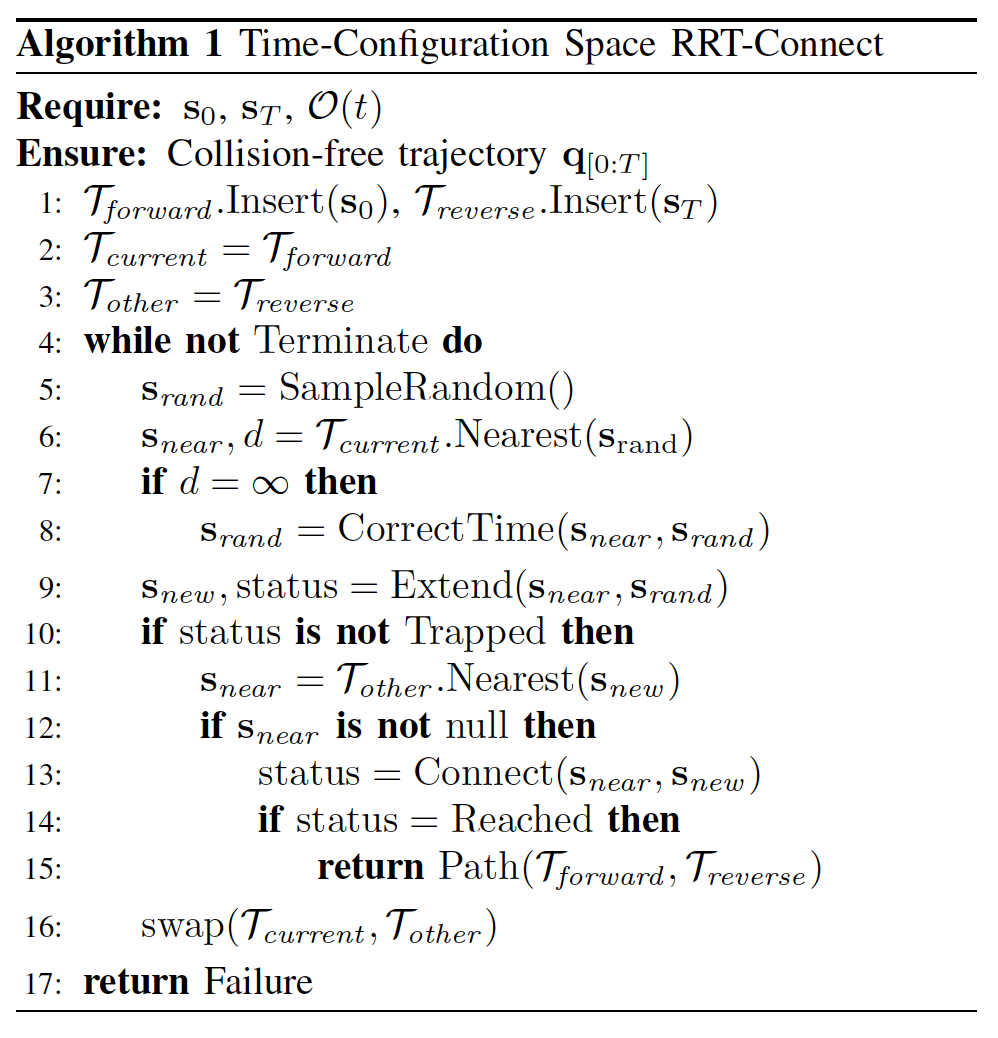
\includegraphics[width=0.45\linewidth]{algorithms/time_rrt_algo.png}
                \centering
                \label{fig:time_rrt_algo}}
                \quad
                \subfigure[Example of Time-Configuration RRT-Connect\cite{yang_planning_2018}]{
                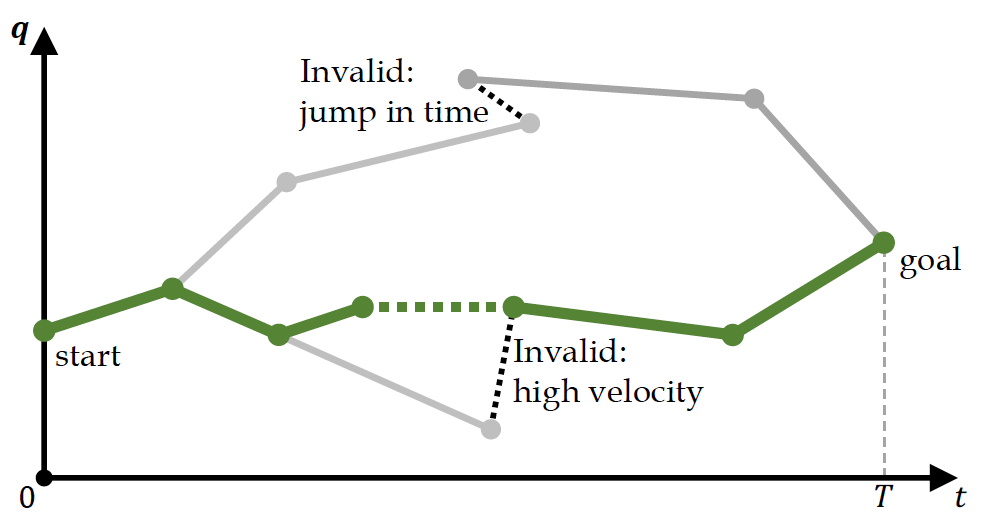
\includegraphics[width=0.45\linewidth]{algorithms/time_rrt.png}
                \centering
                \label{fig:time_rrt_image}}
                \caption{Time-Configuration RRT-Connect}
                \label{fig:time_rrt}
            \end{figure}

        \subsubsection{Time-Configuration Space RRT-Connect}
            Reach planning in the presence of time-varying obstacle trajectories searches for a path in time-configuration space. This space includes a time parameter in addition to the entire configuration space of the robot. The time parameter is constrained by velocity and temporal constraints. The velocity constraint ensures that joint velocity limits are not exceeded. The temporal constraint ensures causality/time-monotonicity, so the robot does not travel backward in time. Similar to the case in CBiRRT2, the sample space may be of a higher dimension than the constraint manifold, so rejection sampling does not work efficiently. This issue is further exaggerated by the introduction of the dimension of time. \cite{yang_planning_2018} introduces a CorrectTime function that works by adjusting the time parameter after a valid sample is chosen from the free configuration space. The time parameter is adjusted based on a custom distance function that only returns a real value if both time constraints are satisfied. [Reference figure 3 of time-indexed PPP*** reference].

        \subsubsection{Optimization-Based Planning}
            The grasping is solved for by a non-linear programming solver such as SNOPT and AICO. As SNOPT is a proprietary, licensed software, AICO is used for this project. AICO is a method of path planning that falls into the trajectory optimization category, unlike the sampling-based planners described so far.

        \subsubsection{Approximate Inference Control}
            Approximate Inference Control (AICO) \cite{toussaint_robot_2009} builds on Iterative Linear-Quadratic-Gaussian (iLQG) which is a method of sequential quadratic programming \cite{todorov_generalized_2005}. iLQG stems from the basic linear-quadratic gaussian control(LQG).

            \par A linear-quadratic (LQ) problem deals with a system with dynamics that are described by linear differential equations and with a quadratic cost. An LQG control problem assumes additive, white Gaussian noise on both the state of the system as well as the measurement of the system state. An LQG controller is a control law that uses a Kalman filter for state estimation and a Linear-Quadratic Regulator (LQR) for feedback control. The LQG controller succeeds at identifying the current state and control variables at a given instant to bring the controlled process variable to the desired reference point.

            The following extensions on LQG control use the principle of dynamic programming to extend LQG control to entire trajectories. Dynamic programming recursively breaks down a large optimization problem into smaller sub-problems using the Bellman equation,
            \begin{equation}
                V(x)=\max_{a \in \Gamma (x)}\{F(x,a)+\beta V(T(x,a))\}
            \end{equation}
            where $x$ is a state of the system and $a$ is a control variable that determines the action taken to reach the next state. $V(x)$ is the optimal value of a state $x$. $\Gamma(x)$ denotes the set of all possible actions that can be taken at state $x$. $T(x,a)$ represents a state transition resulting from control variable $a$ at state $x$. $F(x,a)$ is the value of taking action $a$ at state $x$. $\beta$ is a discount factor that decreases the value of subsequent state transitions. By finding the maximum value of the initial state $x_{o}$ of a system, the optimal policy function $a(x)$ is also found, which describes the optimal action to take at a given state.

            \begin{figure}
                \centering
                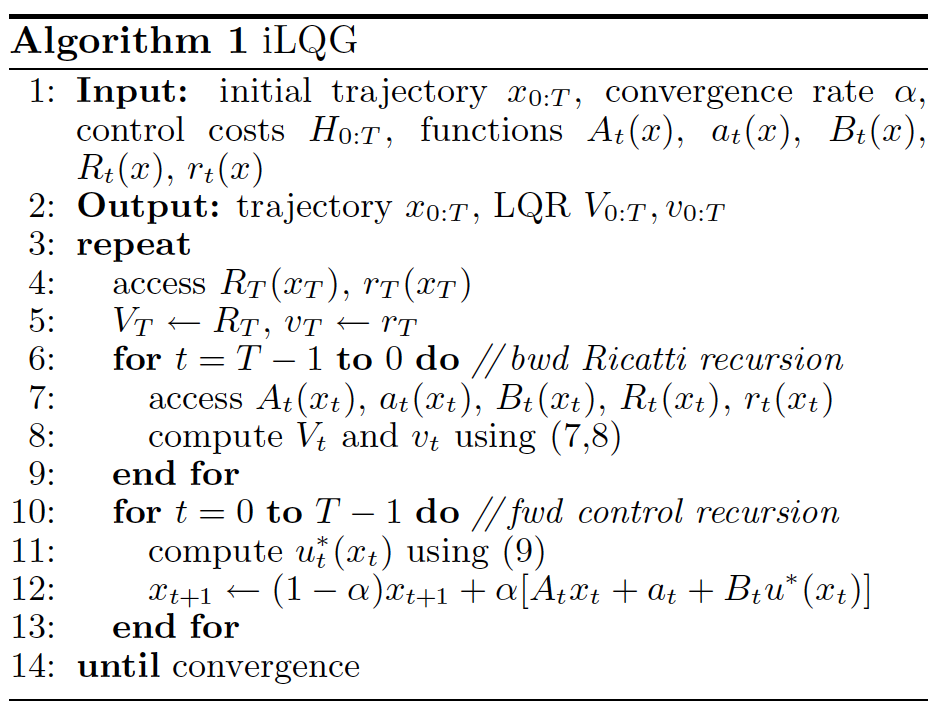
\includegraphics[width=0.45\linewidth]{images/algorithms/ilqg.png}
                \label{fig:ilqg}
                \caption{iLQG Algorithm \protect\cite{todorov_generalized_2005}}
            \end{figure}

            \par iLQG optimizes a control sequence by linearizing the system dynamics around each system state and control input in the sequence. This local linearization casts the non-linear system dynamics problem into a sequence of LQG problems, where each iteration steps through the sequence to further optimize the entire trajectory.The iLQG algorithm utilizes a forward-backward algorithm. iLQG computes a trajectory with a forward pass by applying a sequence of control inputs in an open-loop manner. A backward pass recursively calculates the cost-to-go function, much like in the Bellman equation, except that the cost-to-go function is minimized instead of maximizing a value function. Each iteration of the backward step computes a new $a(x)$, which is applied open-loop in the subsequent forward pass. Iterating iLQG until convergence results in a locally optimal trajectory and a linear-quadratic regulator that can handle small perturbations around the selected trajectory.\cite{todorov_generalized_2005} iLQG computed updates to the entire trajectory with each pass
            % A backward pass computes a second-order approximation of the cost-to-go of the trajectory, which is minimized to find a locally optimal trajectory and a linear-quadratic regulator that can handle small perturbations around the selected trajectory. Adjustments are made to the sequence of control inputs in the subsequent forward pass until the trajectory converges. The iLQG method minimizes a cost function to determine a locally optimal trajectory. 

            \begin{figure}
                \centering
                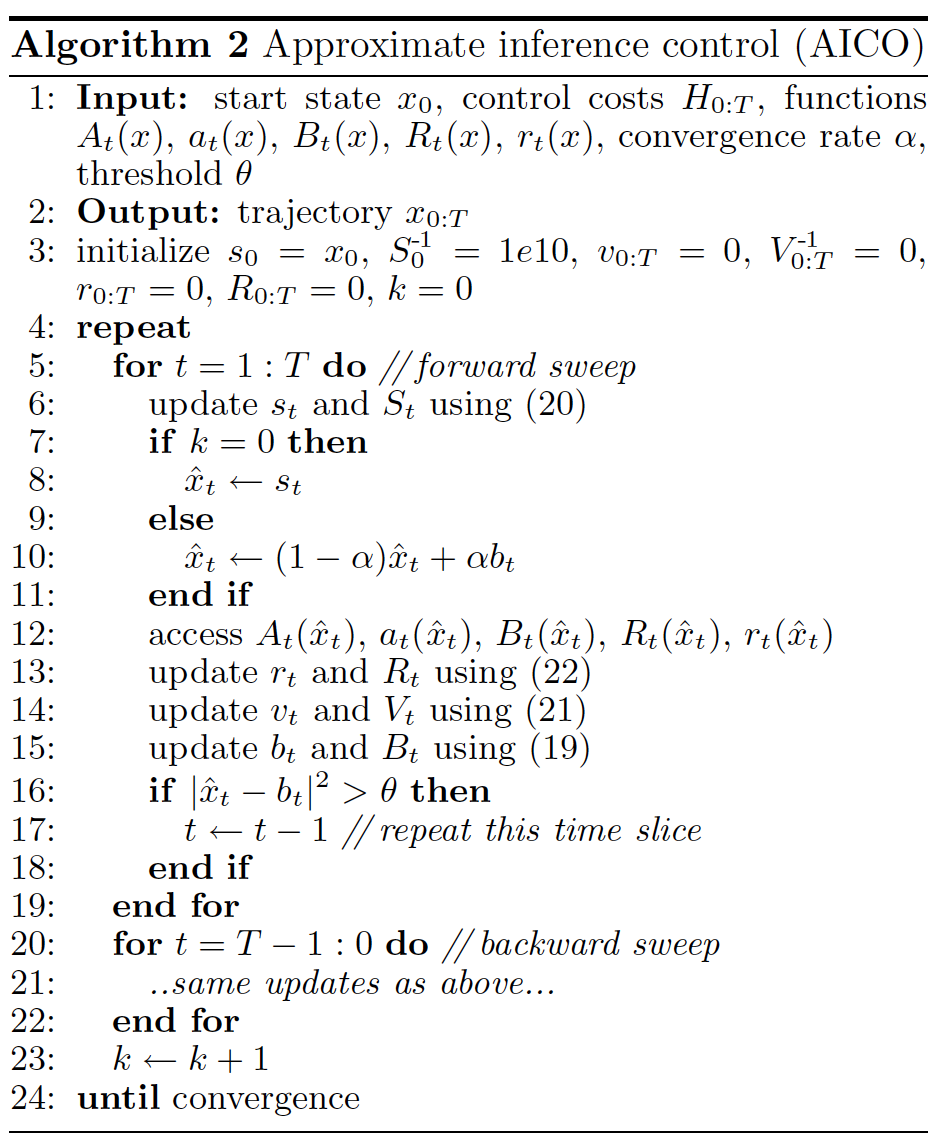
\includegraphics[width=0.45\linewidth]{images/algorithms/aico.png}
                \caption{AICO Algorithm \protect\cite{toussaint_robot_2009}}
                \label{fig:aico}
            \end{figure}

            \par On the other hand, AICO takes a probabilistic inference approach by conditioning a trajectory on constraint conditions. Toussaint demonstrates that for the LQG case, the maximum likelihood trajectory approaches the solution found by cost minimization. AICO uses message-passing to propagate beliefs. In belief propagation, a selected node receives messages from parent nodes, who receive messages from their parent nodes, and so on. This propagation of information updates the selected node with information from the entire network. Then, the selected node distributes messages to its parent nodes, which redistributes information throughout the network. \cite{minka_expectation_nodate}
            \par For trajectories, the network centers around a single chain where each node represents a time step. In AICO, beliefs are the product of received messages,
            \begin{equation}
                b(X)=\prod_{i}t_{i}(X)
            \end{equation}
            where $X$ is a random variable for which belief is expressed. $t$ is assumed to be Gaussian for the LQG case, resulting in $b$ also being Gaussian. The algorithm starts with approximations of $t$ and thus also of $b$. Beliefs are updated by updating approximate messages according to exact messages computed by a simulator.
            Because of message-passing, AICO can linearize around a configuration in the trajectory instead of linearizing around the entire trajectory in the case of iLQG.\cite{toussaint_robot_2009} It is demonstrated in \cite{toussaint_robot_2009} that AICO consistently performs better than iLQG in terms of computation time to convergence.
        % include a comparison between sampling and optimization methods.
        \subsubsection{Commentary}
            \par Sampling-based planners are designed to adeptly search high dimensional configuration spaces without the high computation power required for dynamic programming [Bellman, 1957]. Due to the probabilistic completeness that arises from the process of randomly sampling configurations, sampling-based planners can also better avoid the issue of becoming trapped in a local minima as in the case of gradient-descent approaches such as AICO. However, the task of keeping an end-effector centered on a target object involves multiple differentiable constraints that sampling-based planners are not able to satisfy. Also, paths planned by sampling are often not optimal due to the nature of random sampling. Optimization-based planners generally produce smooth and optimal motion.
            % [Toussaint] notes that it is difficult to include collision avoidance in AICO and describes that in practice the trajectory optimization would be based on a physical simulator. 
            Yang, Merkt, et.al. explain that the solver gets easily trapped in local minima in static environments under collision constraints. They elect to solve grasping trajectories until a collision-free trajectory is found. \cite{yang_planning_2018} implemented their pick-and-place framework in the Extensible Optimization Toolset (EXOTica) framework \cite{koubaa_exotica_2019}. EXOTica is "a framework of software tools designed for development and evaluation of motion synthesis algorithms within ROS" and includes an implementation of motion solvers such as AICO as a benchmark for new motion planning algorithms.\cite{koubaa_exotica_2019} This project uses EXOTica to plan the grasping phase of the drive-by pick-and-place motion. Further details on the EXOTica framework are provided below.
    \newpage
    \section{Method/Approach}
        \begin{figure}
            \centering
            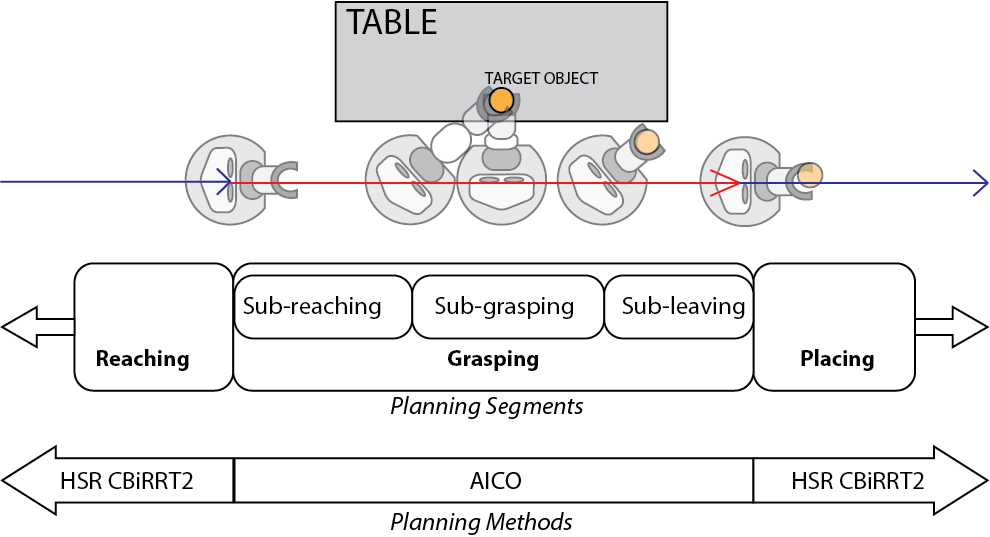
\includegraphics[width=0.95\linewidth]{illustrator/segments.png}
            \label{fig:segments}
            \caption{Planning Overview}
        \end{figure}
        \subsection{Overview}
            This project closely follows the method proposed in \cite{yang_planning_2018}. One significant difference is that the time-configuration planning method is designed for picking and placing a moving object. A drive-by pick-and-place scenario also has the target object moving relative to the robot, but in the drive-by case, the HSR must approximately follow a predefined trajectory which complicates the end-effector tracking of the object during the grasping phase as shown in \cref{fig:driveby}. This issue is largely due to the limited reachability of the HSR arm. To address this issue, the grasping phase is allotted an extended duration of time to encompass the HSR's approach and grasping of the object as depicted in \cref{fig:segments}. The new, extended grasping phase plans the sub-reaching, sub-grasping, and sub-leaving steps as shown in \cref{fig:segments}.
            % The HSR CBiRRT2 variant is used to reach the start of the extended grasping phase and leave from the end pose of the extended grasping phase to place the object. 

            \par This method differs from the Time-Configuration RRT-Connect in that the grasping phase is extended to incorporate a sub-reaching, sub-grasping, and a sub-leaving stage while maintaining the reaching and placing phases. The reaching segment brings the HSR to the start pose for the grasping segment and the placing segment starts from the end pose of the grasping segment, like in \cite{yang_planning_2018}. At the start of the grasping segment, the sub-reaching phase brings the HSR gripper end-effector to the soda can. In the sub-grasping phase, the gripper remains around the soda can as the HSR base moves, for long enough to close the gripper aroiund the soda can. In the sub-leaving phase, the HSR drives to the start pose of the placing segment.

            \par The HSR CBiRRT2 variant is used to reach the start of the  grasping segemnt and leave from the end pose of the extended grasping segment to place the object. This is largely for convenience. The HSR CBiRRT2 planning algorithm is built-in on the robot and the world is static for this project. The time-varying component of the problem is the position of the target object, a soda can in this instance, relative to the HSR as it drives-by, following a trajectory. 
            % It is assumed that computing a collision-free drive-by base trajectory for the HSR is trivial, using Time-Configuration space planning methods detailed in [***]. Therefore, the reaching and placing motions around dynamic obstacles are already accounted for in the given base trajectory and can be replaced by HSR motion planning for demonstration purposes. 
            The extended grasping step can be planned using AICO and activating specific constraints during the sub-grasping phase time window.
        
            The HSR CBiRRT2 motion planning algorithm is already implemented on the HSR and TOPP allows for control over the timing of planned trajectories. This covers the reaching and placing steps of the motion plan. The key step for this project is planning a whole-body trajectory for the extended grasping segment, which is covered in the remainder of this paper.
        
        \begin{figure}
            \centering
            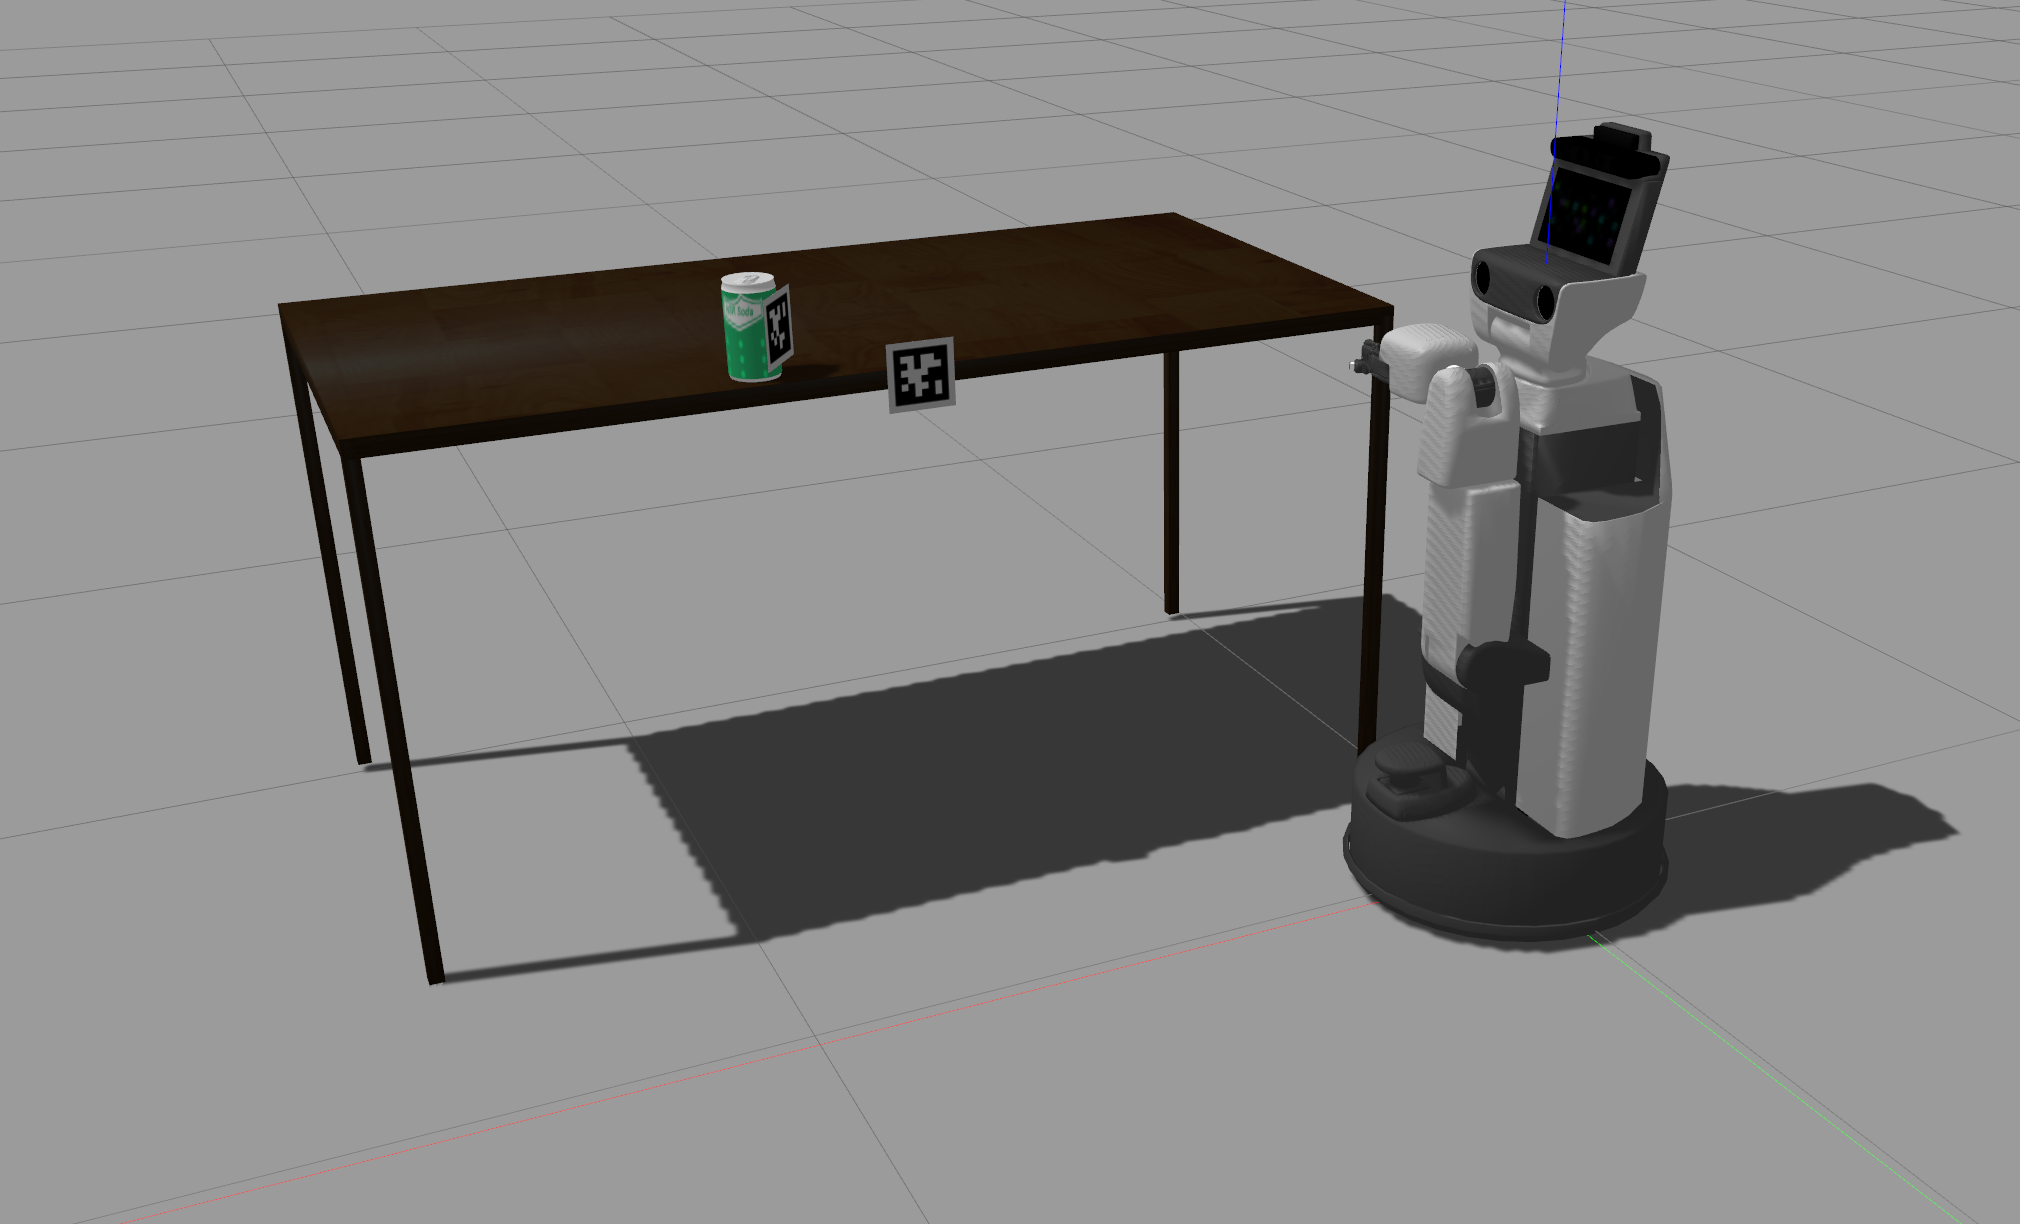
\includegraphics[width=0.95\linewidth]{2020.05.19/setup.png}
            \label{fig:problem_setup}
            \caption{Testing environment for the grasping segment in Gazebo simulation}
        \end{figure}

        \subsection{Scenario Setup}
            To simplify the problem described in Section 5.1, a bare-bones world containing only an Ikea Nyboda Table and a soda can was created in Gazebo. Gazebo is an open-source robotics simulator commonly used for ROS-based robot simulations.\cite{koenig_design_2004} The objects in the simplified scenario were chosen for convenience. The Ikea Nyboda Table was chosen as it was the model of table present in the testing space for the HSR. A soda can was chosen as the target pick-and-place object since it is a household item and a representative task for a service robot. Further, the radius of the soda can is larger than items expected to be used in real-world testing, which produces a scenario with a smaller margin for error in terms of end-effector positioning. <insert figure>. In this example, the HSR follows a given base trajectory that is parallel to the table and attempts to grasp the bottle.
            
        \subsection{Constraints On Grasping}
            The grasping method in \cite{yang_planning_2018} identifies valid grasping trajectories by generating new trajectories using AICO until a collision-free trajectory is found. In those cases, the grasping phases have a relatively short time frame. For instance, the HSR can close its gripper within 0.4 seconds, giving a maximum grasping duration of 0.4 seconds. In the case of the extended grasping phase for the drive-by problem, the duration for the HSR is around 15 seconds. Although computation time depends on the number of waypoints in a trajectory, the distances traversed are much larger in the case of the drive-by problem. This means that checking for collisions after computing trajectories is no longer efficient since it is highly likely that the arm or end effector would collide with the table in this test scenario. To accommodate for this issue, constraints are introduced to reduce the likelihood of colliding with the table. As mentioned above, EXOTica is used to plan this grasping phase.

        \subsection{EXOTica}
            As a benchmark framework, EXOTica introduces abstractions that separate a problem into 3 components so multiple motion solvers can be used to compare efficiency.\cite{koubaa_exotica_2019} The components are a planning scene, a planning problem, and a motion solver.[ref]
                
            \par The planning scene contains information about the robot and its environment. In the test example, the planning scene contains the position and geometry of the Nyboda table, and soda can as well as information about the HSR. This environment is read from a file with a .scene file format. The HSR dynamics and kinematic properties are read from URDF and SRDF files. (Unified Robot Description Format and Semantic Robot Description Format)[probably some reference to the file formats]. The base trajectory for the drive-by is also specified here since it defines the robot's base position in the scene. This input base trajectory acts as a base position and orientation constraint.

            \par The motion solver is set as AICO since the purpose of this project is to use the motion solver implementation instead of benchmarking a new solver. It is important to note that AICO does not guarantee that constraints are satisfied. Instead, it optimizes the trajectory according to a quadratic cost function, in which each constraint is weighted according to its cost.

            \par The planning problem defines the type of problem being solved and the tasks to be completed. The problem definition used for the grasping phase is an Unconstrained Time-Indexed Problem since it defines a 'defines a problem minimizing the quadratic cost over a trajectory using a kinematic model of the system', which can be solved by AICO. The planning problem uses task maps, which are functions that map the configuration space to task space. EXOTica includes several common taskmaps that are utilized in this project to define constraints on the HSR during the grasping phase.
            
            \begin{figure}[ht]
                \centering
                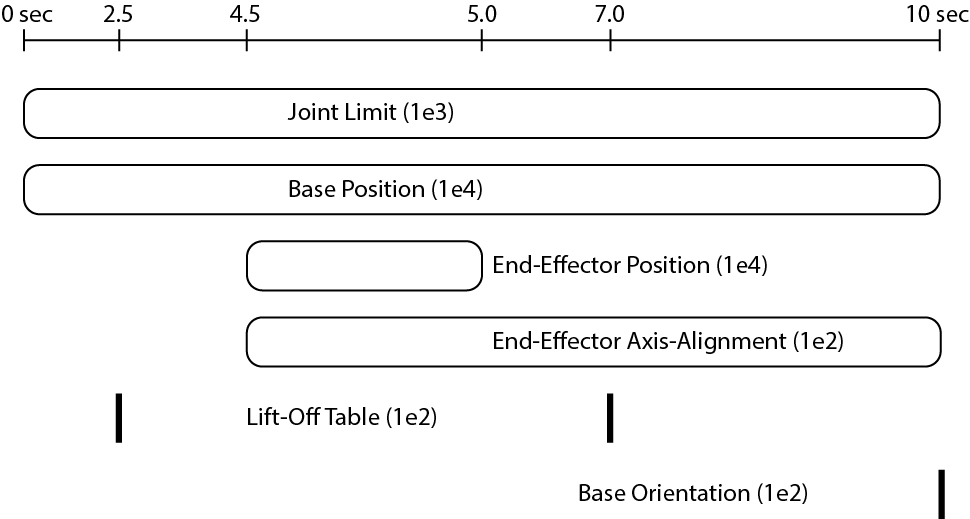
\includegraphics[]{illustrator/taskmap.png}
                \label{fig:taskmap}
                \caption{A graphical depiction of the timing of taskmap activation. Elongated rounded rectangles denote taskmaps that are active for a duration of time. Bars represent task maps that push the HSR to achieve desired values at a point in time. Associated costs for the taskmaps are listed in parenthesis. Greater costs correspond to higher priority.}
            \end{figure}

            \subsubsection{Taskmaps}
                Task maps are active at various points of the extended grasping phase depending on the sub-phase. A task map is considered active when its associated cost is greater than zero. Throughout the entire extended grasping phase, 2 task maps are constantly active:
                \begin{itemize}
                    \item A Joint Limit task map penalizes joint limit violations to promote HSR arm trajectories that fall within viable configurations.

                    \item A Base Position task map penalizes deviations from the drive-by base trajectory specified in the planning scene.
                \end{itemize}

                4 task maps are activated during the sub-grasping phase. Despite the notion that the task maps are active at a certain time, AICO attempts to optimize the trajectory such that the constraint imposed by the task is satisfied in the window of time that the task map is active.
                \begin{itemize}
                    \item An End Effector Position Task map causes the HSR to reach the location of the target soda can object. This task map is activated in the window of the sub-grasping phase. The sub-grasping window is defined by 
                    \[{grasp\ window} = t_{grasp\ start}: t_{grasp\ start}+grasp\  duration\] 
                    where \(t_{grasp\ start}\) is the point in time where the HSR is sufficiently close to reaching the soda can and \({grasp\ duration}\) is the maximum time necessary to close the HSR gripper, which is 0.4 seconds.

                    \item An End-Effector Axis Alignment task map aligns the HSR gripper with the axis of the cylindrical soda can so the gripper stays around the soda can while the fingers of the gripper close. It also prevents the HSR from inverting the soda can. This Axis Alignment task begins at \(t_{grasp\ start}\) and remains active to keep the soda can upright for the remainder of the extended grasping phase.

                    \item A Point to Plane task map named 'Lift Off Table' keeps the end effector a set distance above the plane of the table to avoid the arm and gripper colliding with the table. This task map is active momentarily before \({grasp\ window}\) and momentarily after \({grasp\ window}\) to position the gripper above the table when transitioning from sub-reach to sub-grasp and from sub-grasp to sub-leave, such that the gripper clears the end of the table when lowering the starting arm configuration. This task map results in a swooping motion of the gripper during the sub-grasping phase. This Lift-Off Table task map takes the place of collision checking the trajectory by creating a trajectory that likely does not collide.
                    \item 
                    \item A Base Orientation task map ensures that the HSR omnibase roatation at the end of the grasping segment matches a given value. For the purpose of testing, zero rotation at the end of the trajectory is desired.
                \end{itemize}
            \subsubsection{Commentary on Task Map Weights}
                The costs of the taskmaps shown in \cref{fig:taskmap} were tuned by hand for the given scenario. Base position and end-effector position have the highest associated cost of 1e4, since the actions associated with taskmaps are the most important to the drive-by pick-and-place problem. The base position taskmap makes the HSR follow the given trajectory and the end-effector position taskmap brings the gripper to the soda can object. The End-Effector Axis-Alignment map results in a sub-grasping phase where the gripper is oriented such that the fingers are around the soda can to grip it around the circumference. The Joint Limit and Lift-Off Table lead to valid trajectories that do not exceed positional hardware limitations of the HSR and do not collide with the table obstacle. The base orientation results in a smooth transition to the placing segment.
        \subsection{HSR Controller}
            The AICO solver outputs a trajectory with position waypoints equally spaced in time. The trajectory is specified through a joint trajectory controller in ROS and sent to the HSR. According to the ROS wiki documentation for the joint trajectory controller, a trajectory composed solely of position waypoints is linearly interpolated and results in a trajectory with discontinuous velocities at the waypoints. 
            \par Taking the difference in positions and dividing by the time step produces an array of desired velocities at each waypoint. This results in a spline interpolation that ensures continuity at the velocity level. 

            \par The trajectory is sent separately to the HSR omnibase and arm controllers. A command is sent to the gripper controller to close the gripper at the start of the sub-grasping phase. The ROS actionlib package was used to create omnibase and arm action clients to pass the trajectory to the HSR action server. The HSR python interface was used to send the close gripper command.

        \subsection{Procedure}
            \subsubsection{Hardware and Simulation Specifications}
                The drive-by pick-and-place motions were run on an HSR simulated in Gazebo. Simulations were performed in Ubuntu Linux LTS 16.04 with ROS Kinetic, on an Intel Xenon E-2286M 2.5-4.0 GHz CPU with 32GB 2666MHz RAM.
                
            \subsubsection{Grasping Phase}
                The drive-by base trajectory was defined in the planning scene as a 1.4-meter path parallel to the edge of the table with a duration of 10 seconds and a distance from the edge of the table of 0.35 meters. This trajectory was defined by two waypoints and results in a linear base trajectory that runs parallel to the Nyboda table. [Insert figure of a top-down view of setup in notes]. Since the task maps passed to the AICO solver do not depend on time, the 10-second duration (\cref{fig:taskmap}) can be scaled in time by increasing or reducing the time step between trajectory waypoints of the solved trajectory.

                \par Due to limitations in the reachability of the HSR arm, the target object was placed near the edge of the table to minimize the likelihood of collision with the table.

            \subsubsection{Object Detection}
                Visual markers are used as a fiducial to accurately acquire the position of the table and soda can using computer vision.
                The HSR includes AR marker detection which uses the depth sensor as well as the stereoscopic camera to determine the position of a defined object. However, AprilTags were used instead since AprilTags were found to permit tag detection from a longer range compared to AR markers. \cite{wang_apriltag_2016}.. 

                \par Once the frames of both the table and soda can were determined, a series of transforms using Kinematics and Dynamics Library (KDL)\cite{noauthor_kinematics_nodate} wrapped in EXOTica produced the absolute position and orientation of the table as well as the position of the bottle in the frame of the table.[references] Since the position of the soda can with respect to the table's frame is known, the planning scene utilized in the test example can be used to compute the extended grasping trajectory.
                The absolute position of the table allows the HSR motion planner to reach the start of the extended grasping phase, which is defined in the frame of the table. [Insert Image of tf's in rviz]
                % \begin{figure}[ht][ht]
                %     \centering
                %     \begin{minipage}[b]{0.45\linewidth}
                %     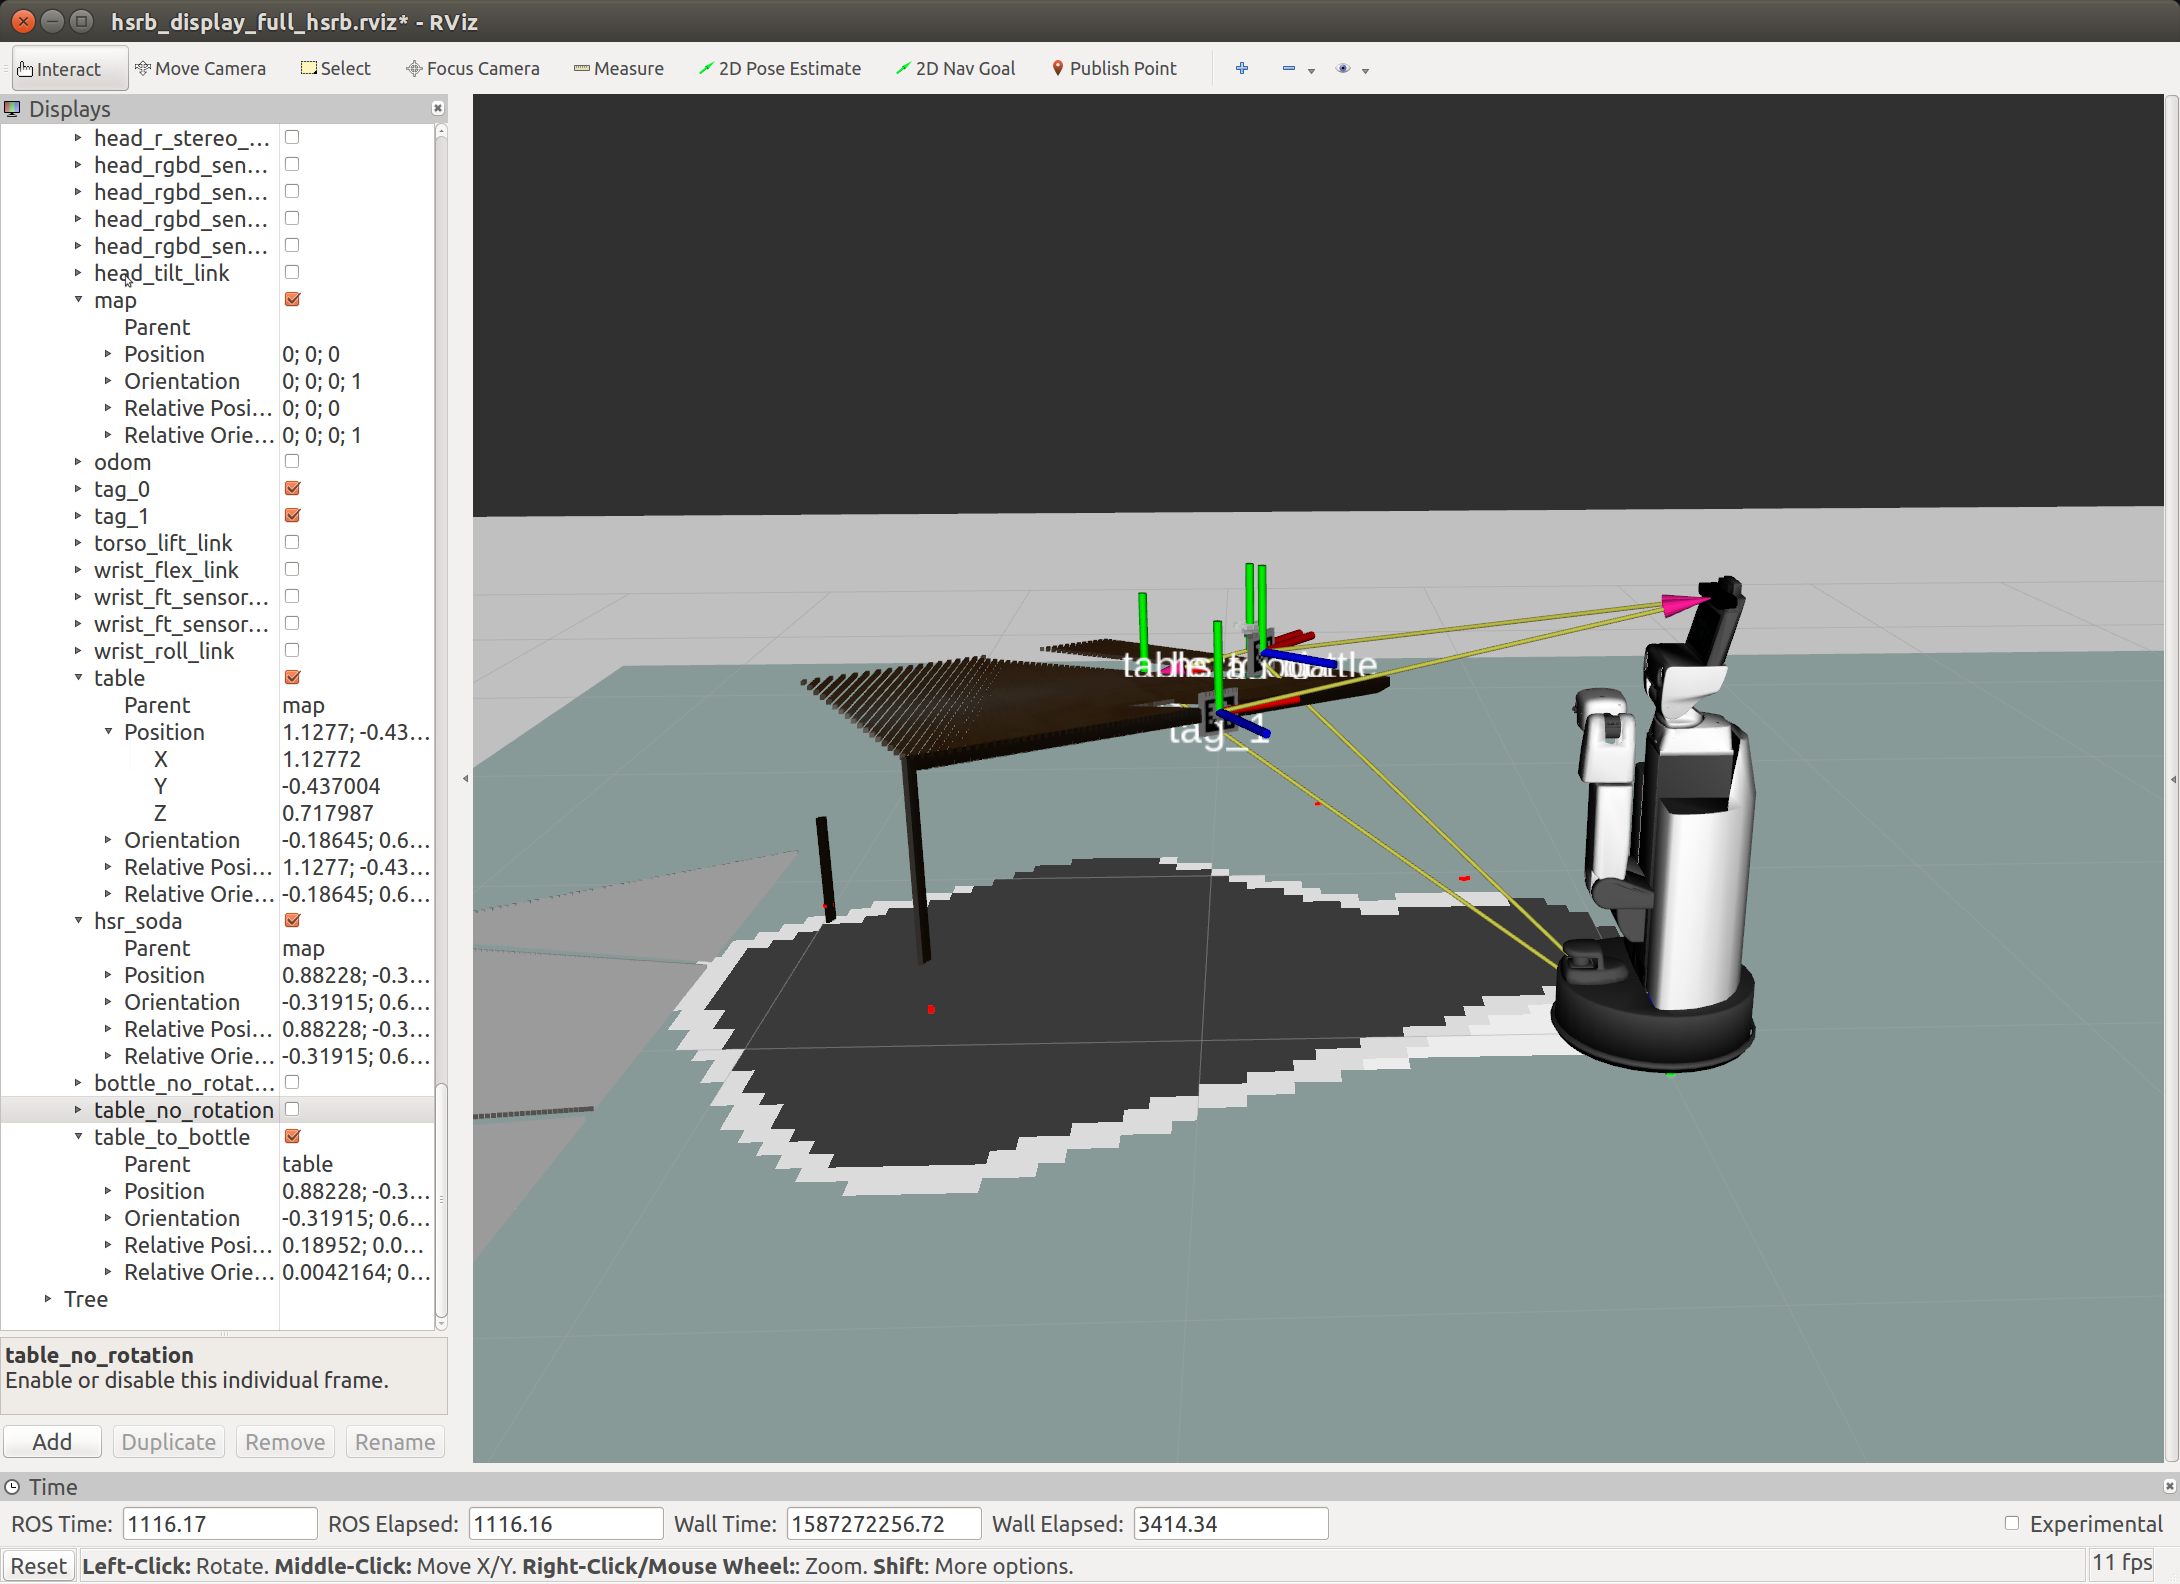
\includegraphics[width=8cm]{2020.04.18/object_locations_rviz.png}
                %     \caption{Will clean up image. Positions of target object and starting base pose for the extended grasping phase.}
                %     \label{fig:minipage1}
                %     \end{minipage}
                %     \quad
                %     \begin{minipage}[b]{0.45\linewidth}
                %     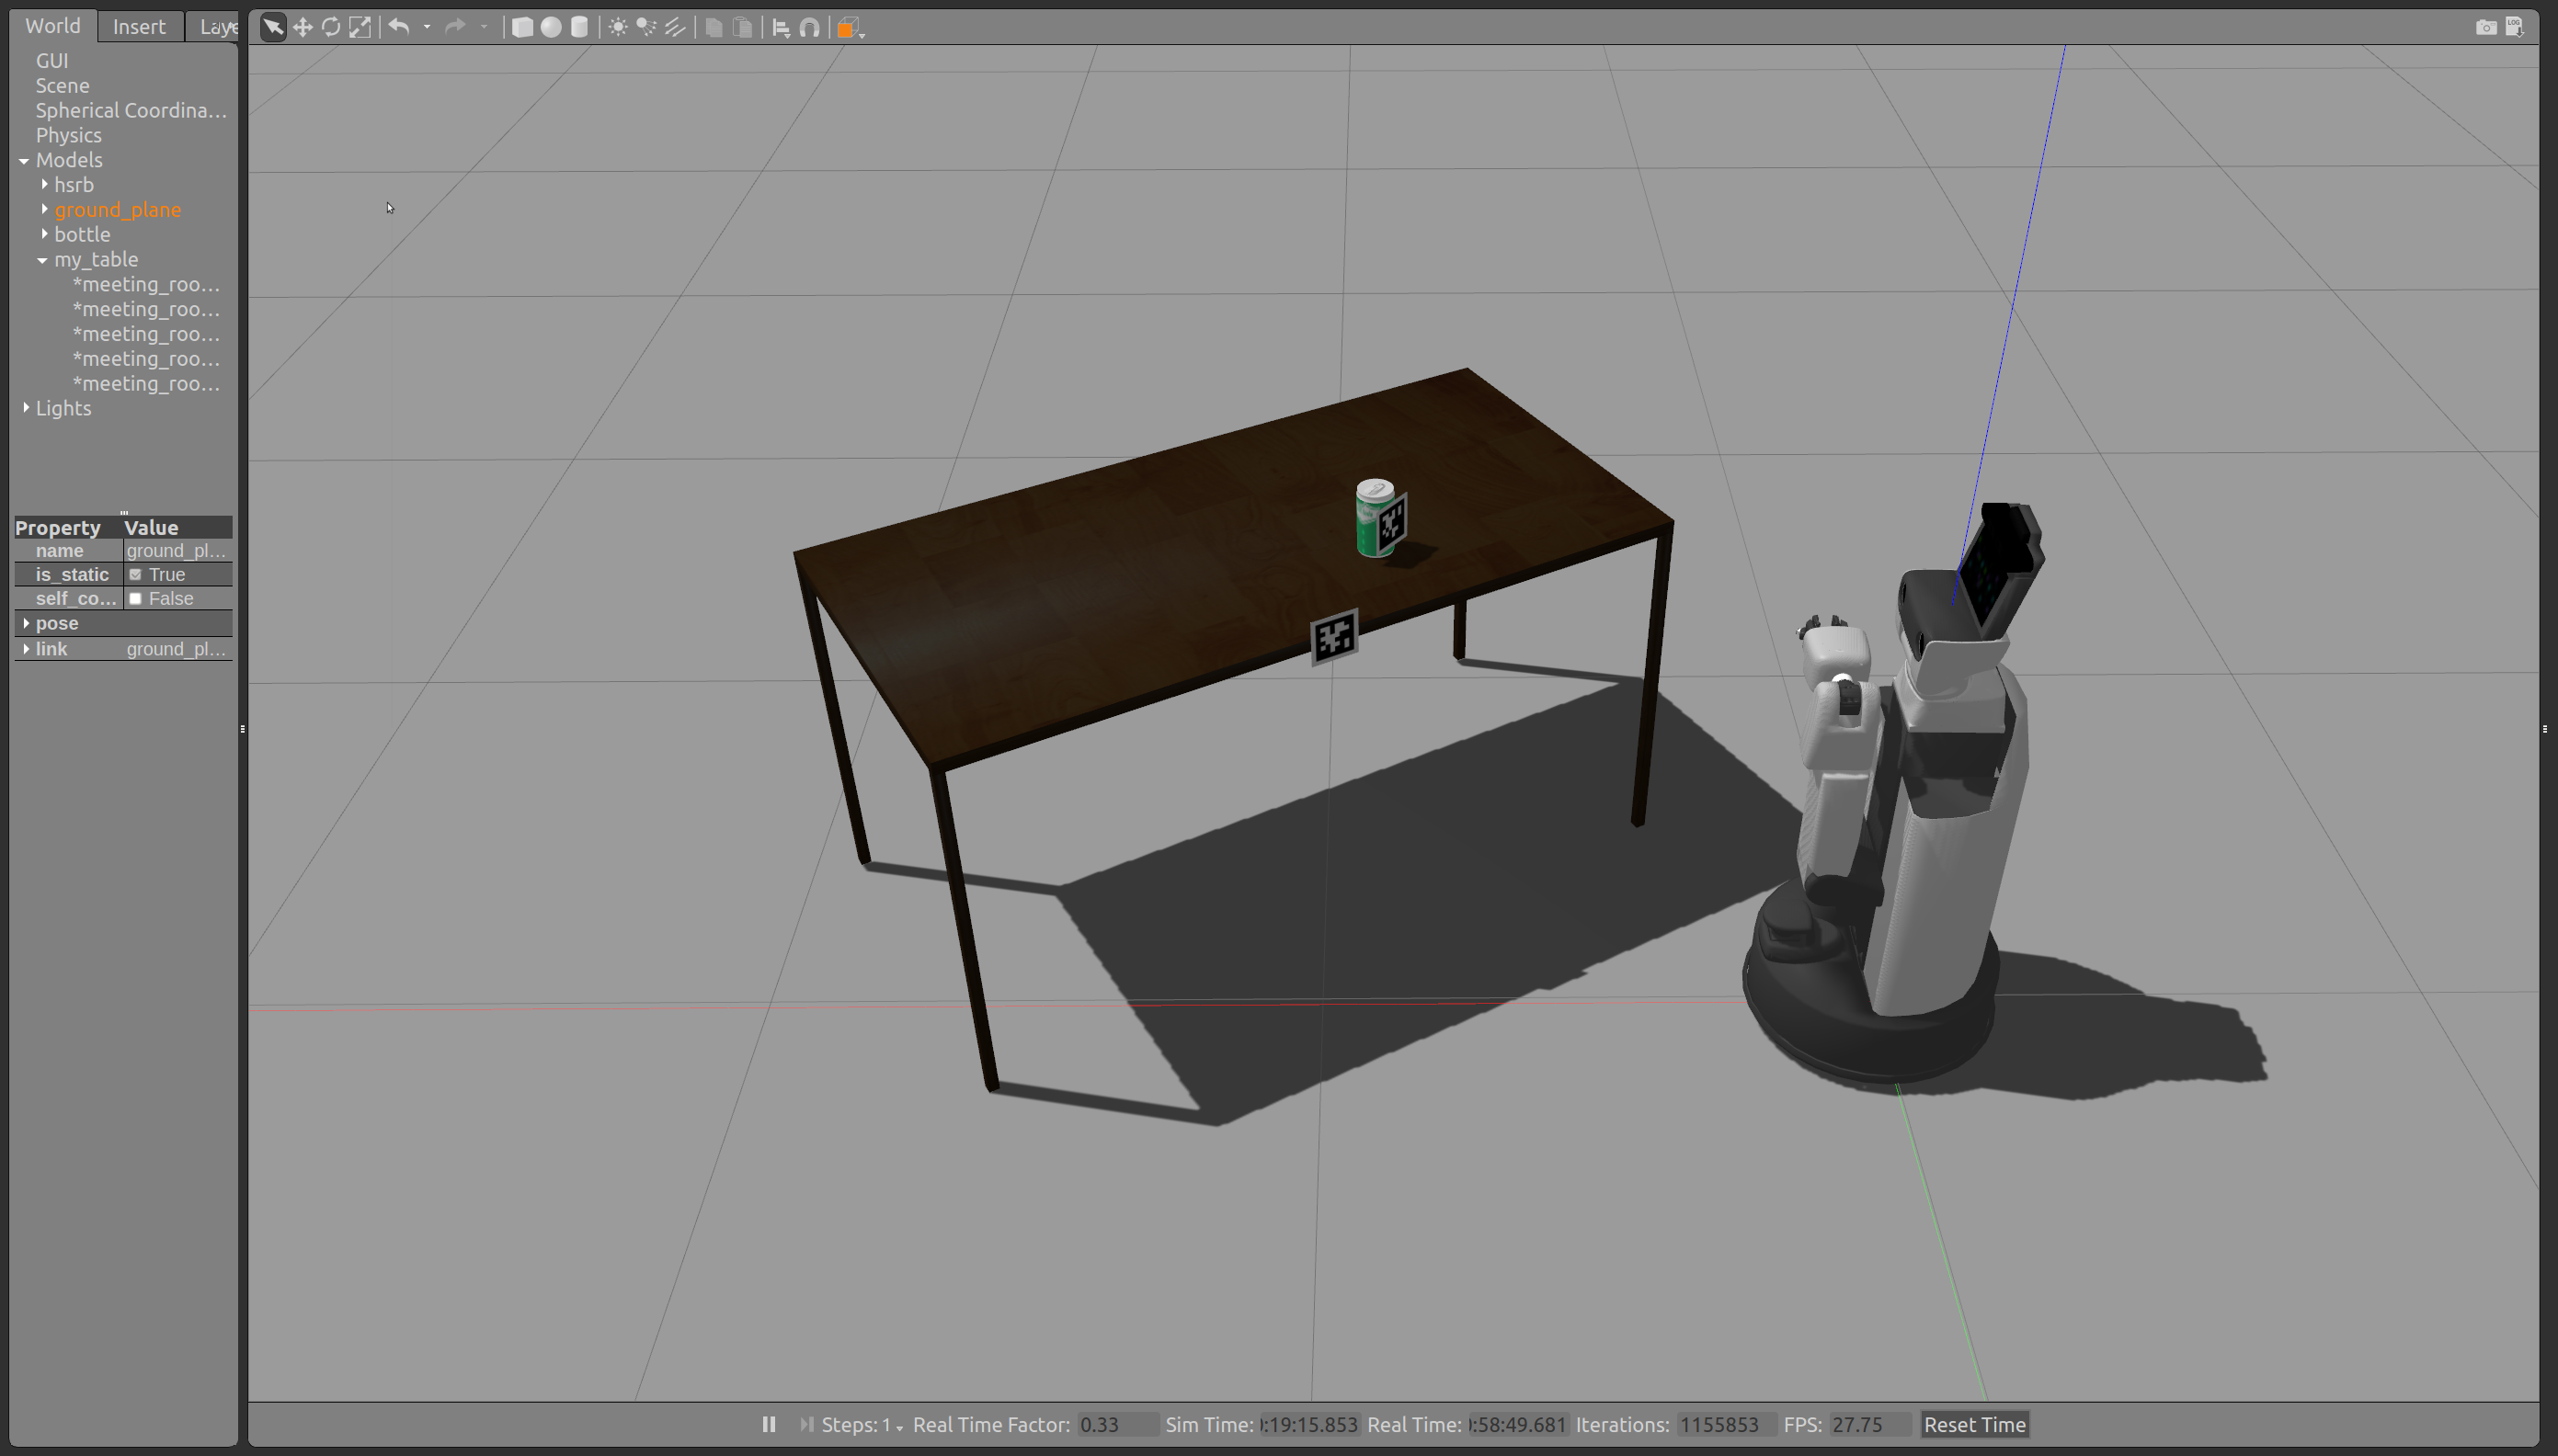
\includegraphics[width=8cm]{2020.04.18/object_locations_gazebo.png}
                %     \caption{Will clean up image. Gazebo visualization of world in Figure 6.}
                %     \label{fig:minipage2}
                %     \end{minipage}
                % \end{figure}
                \begin{figure}[ht]
                    \centering
                    \subfigure[Gazebo Visualization]{%
                    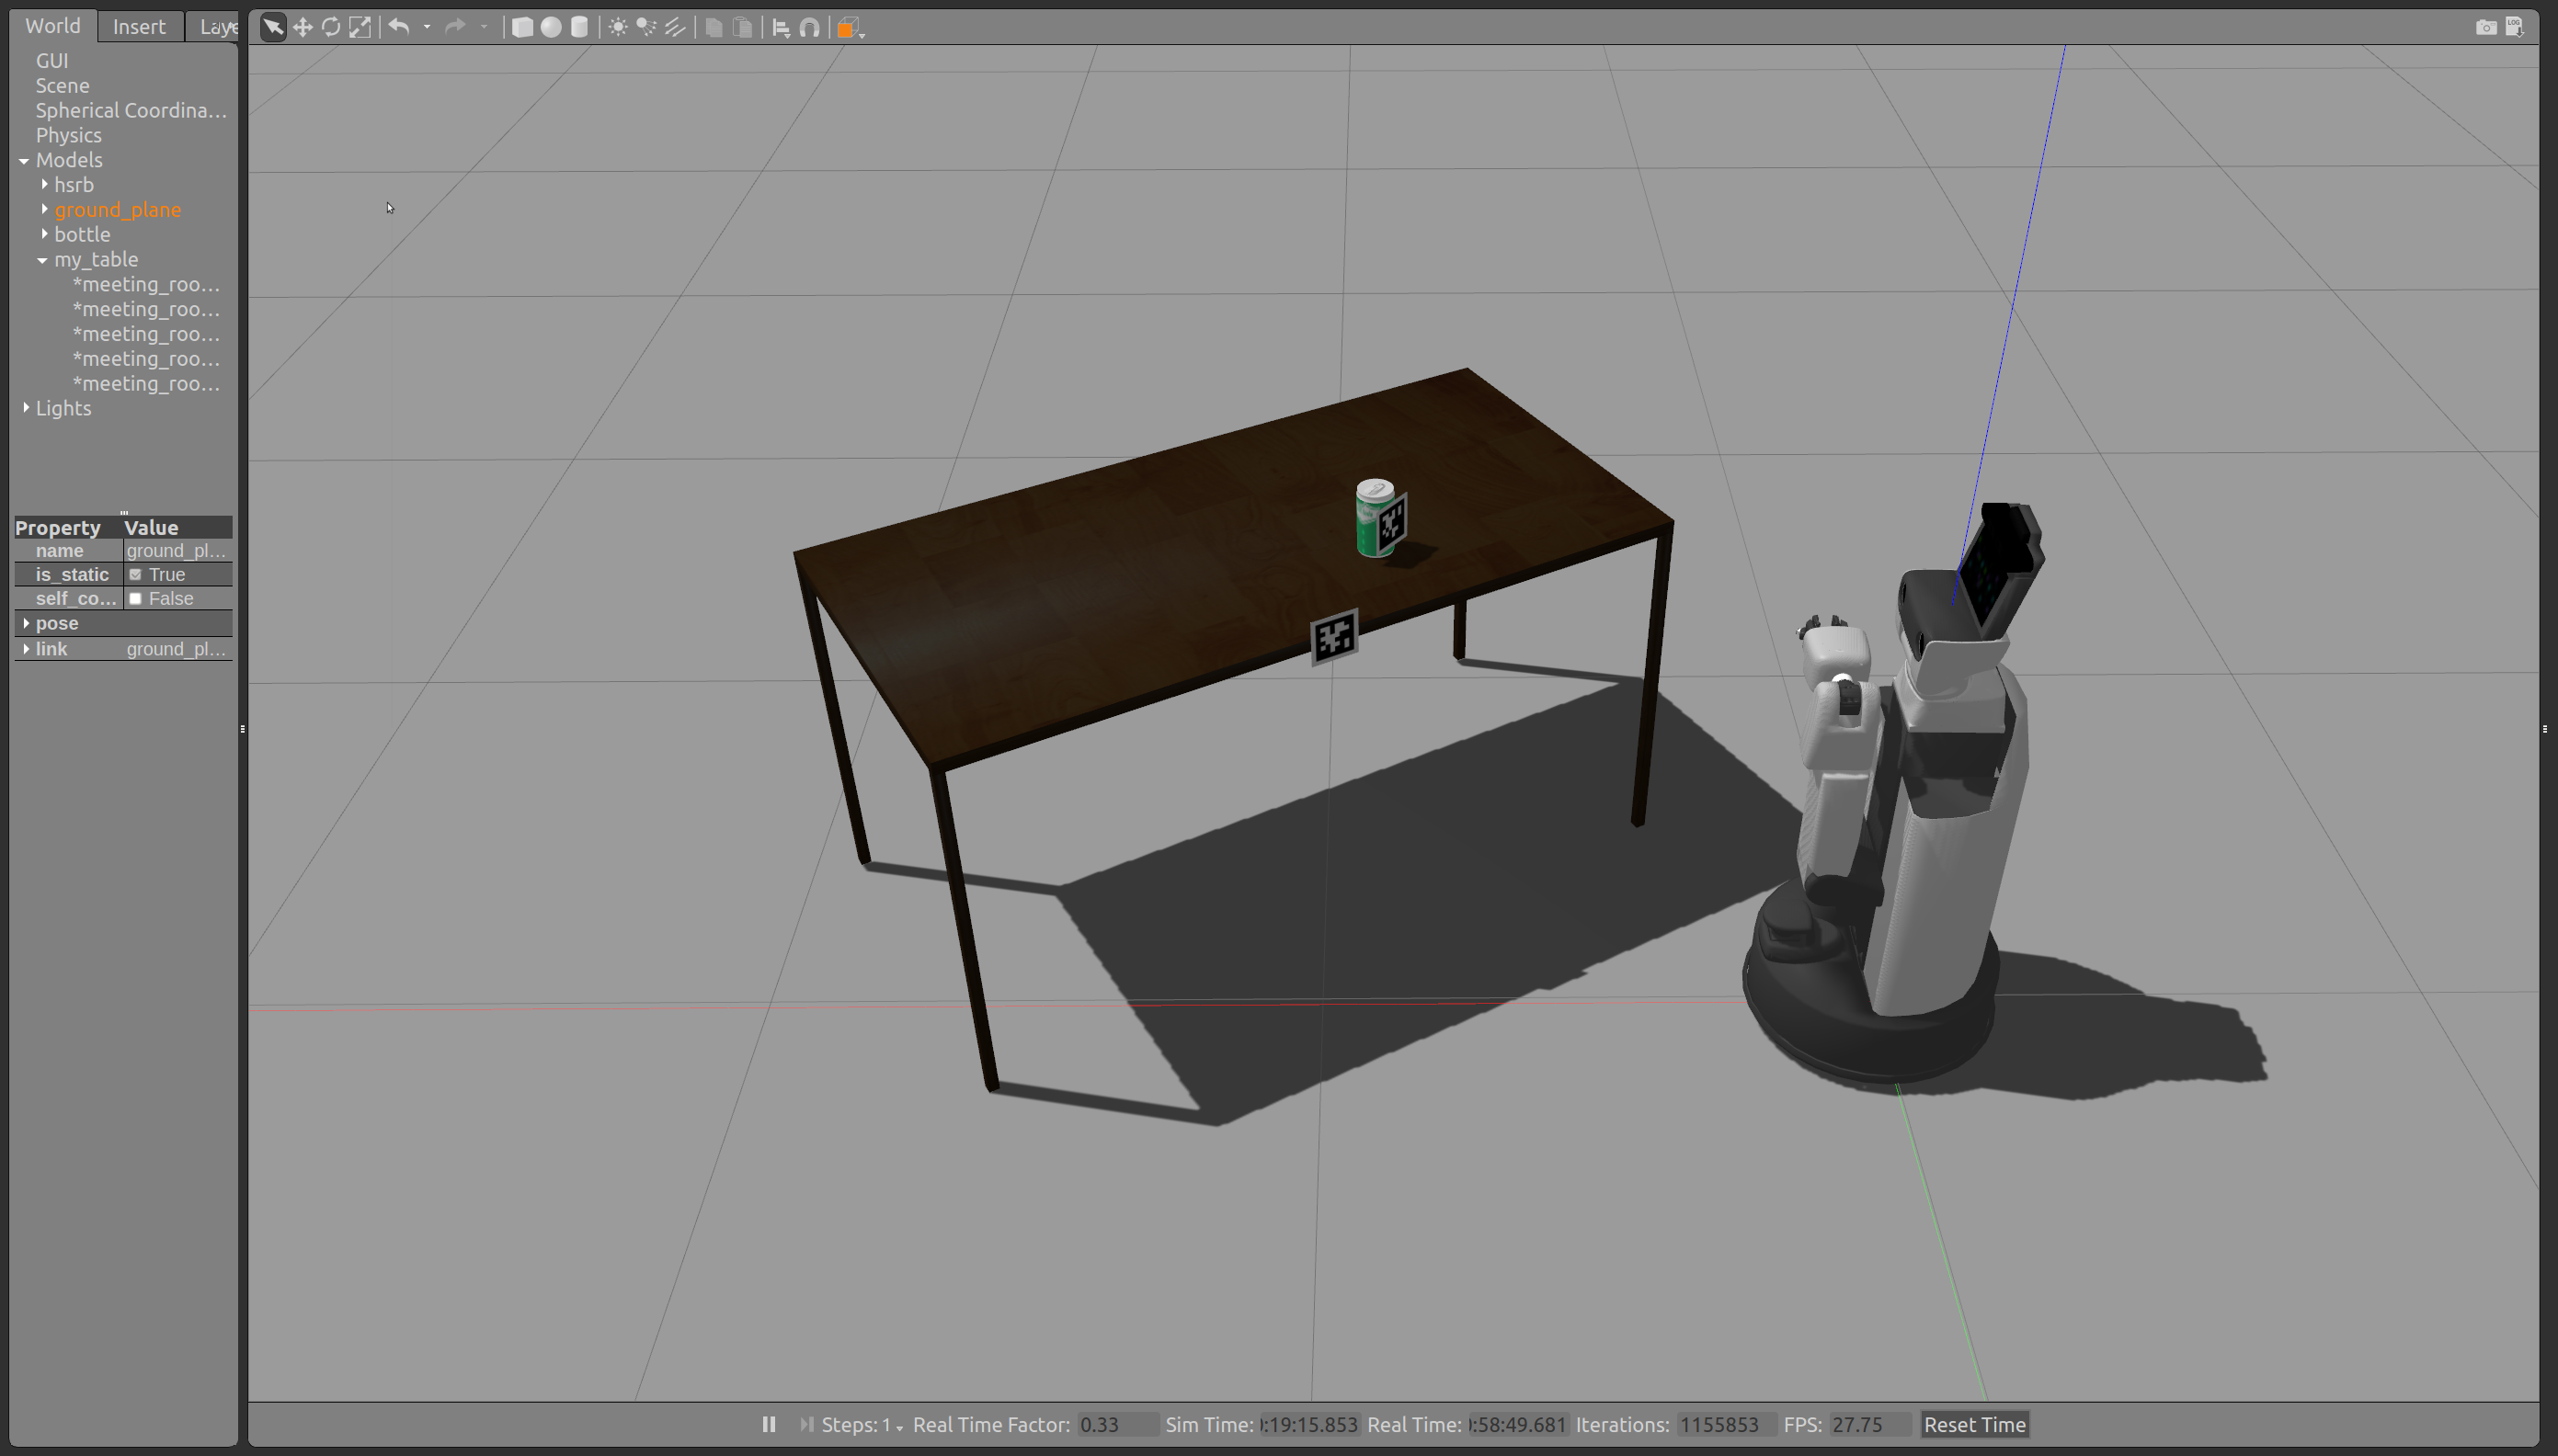
\includegraphics[width=0.45\linewidth]{2020.04.18/object_locations_gazebo.png}
                    \label{fig:subfigure1}}
                    \quad
                    \subfigure[Rviz visualization]{%
                    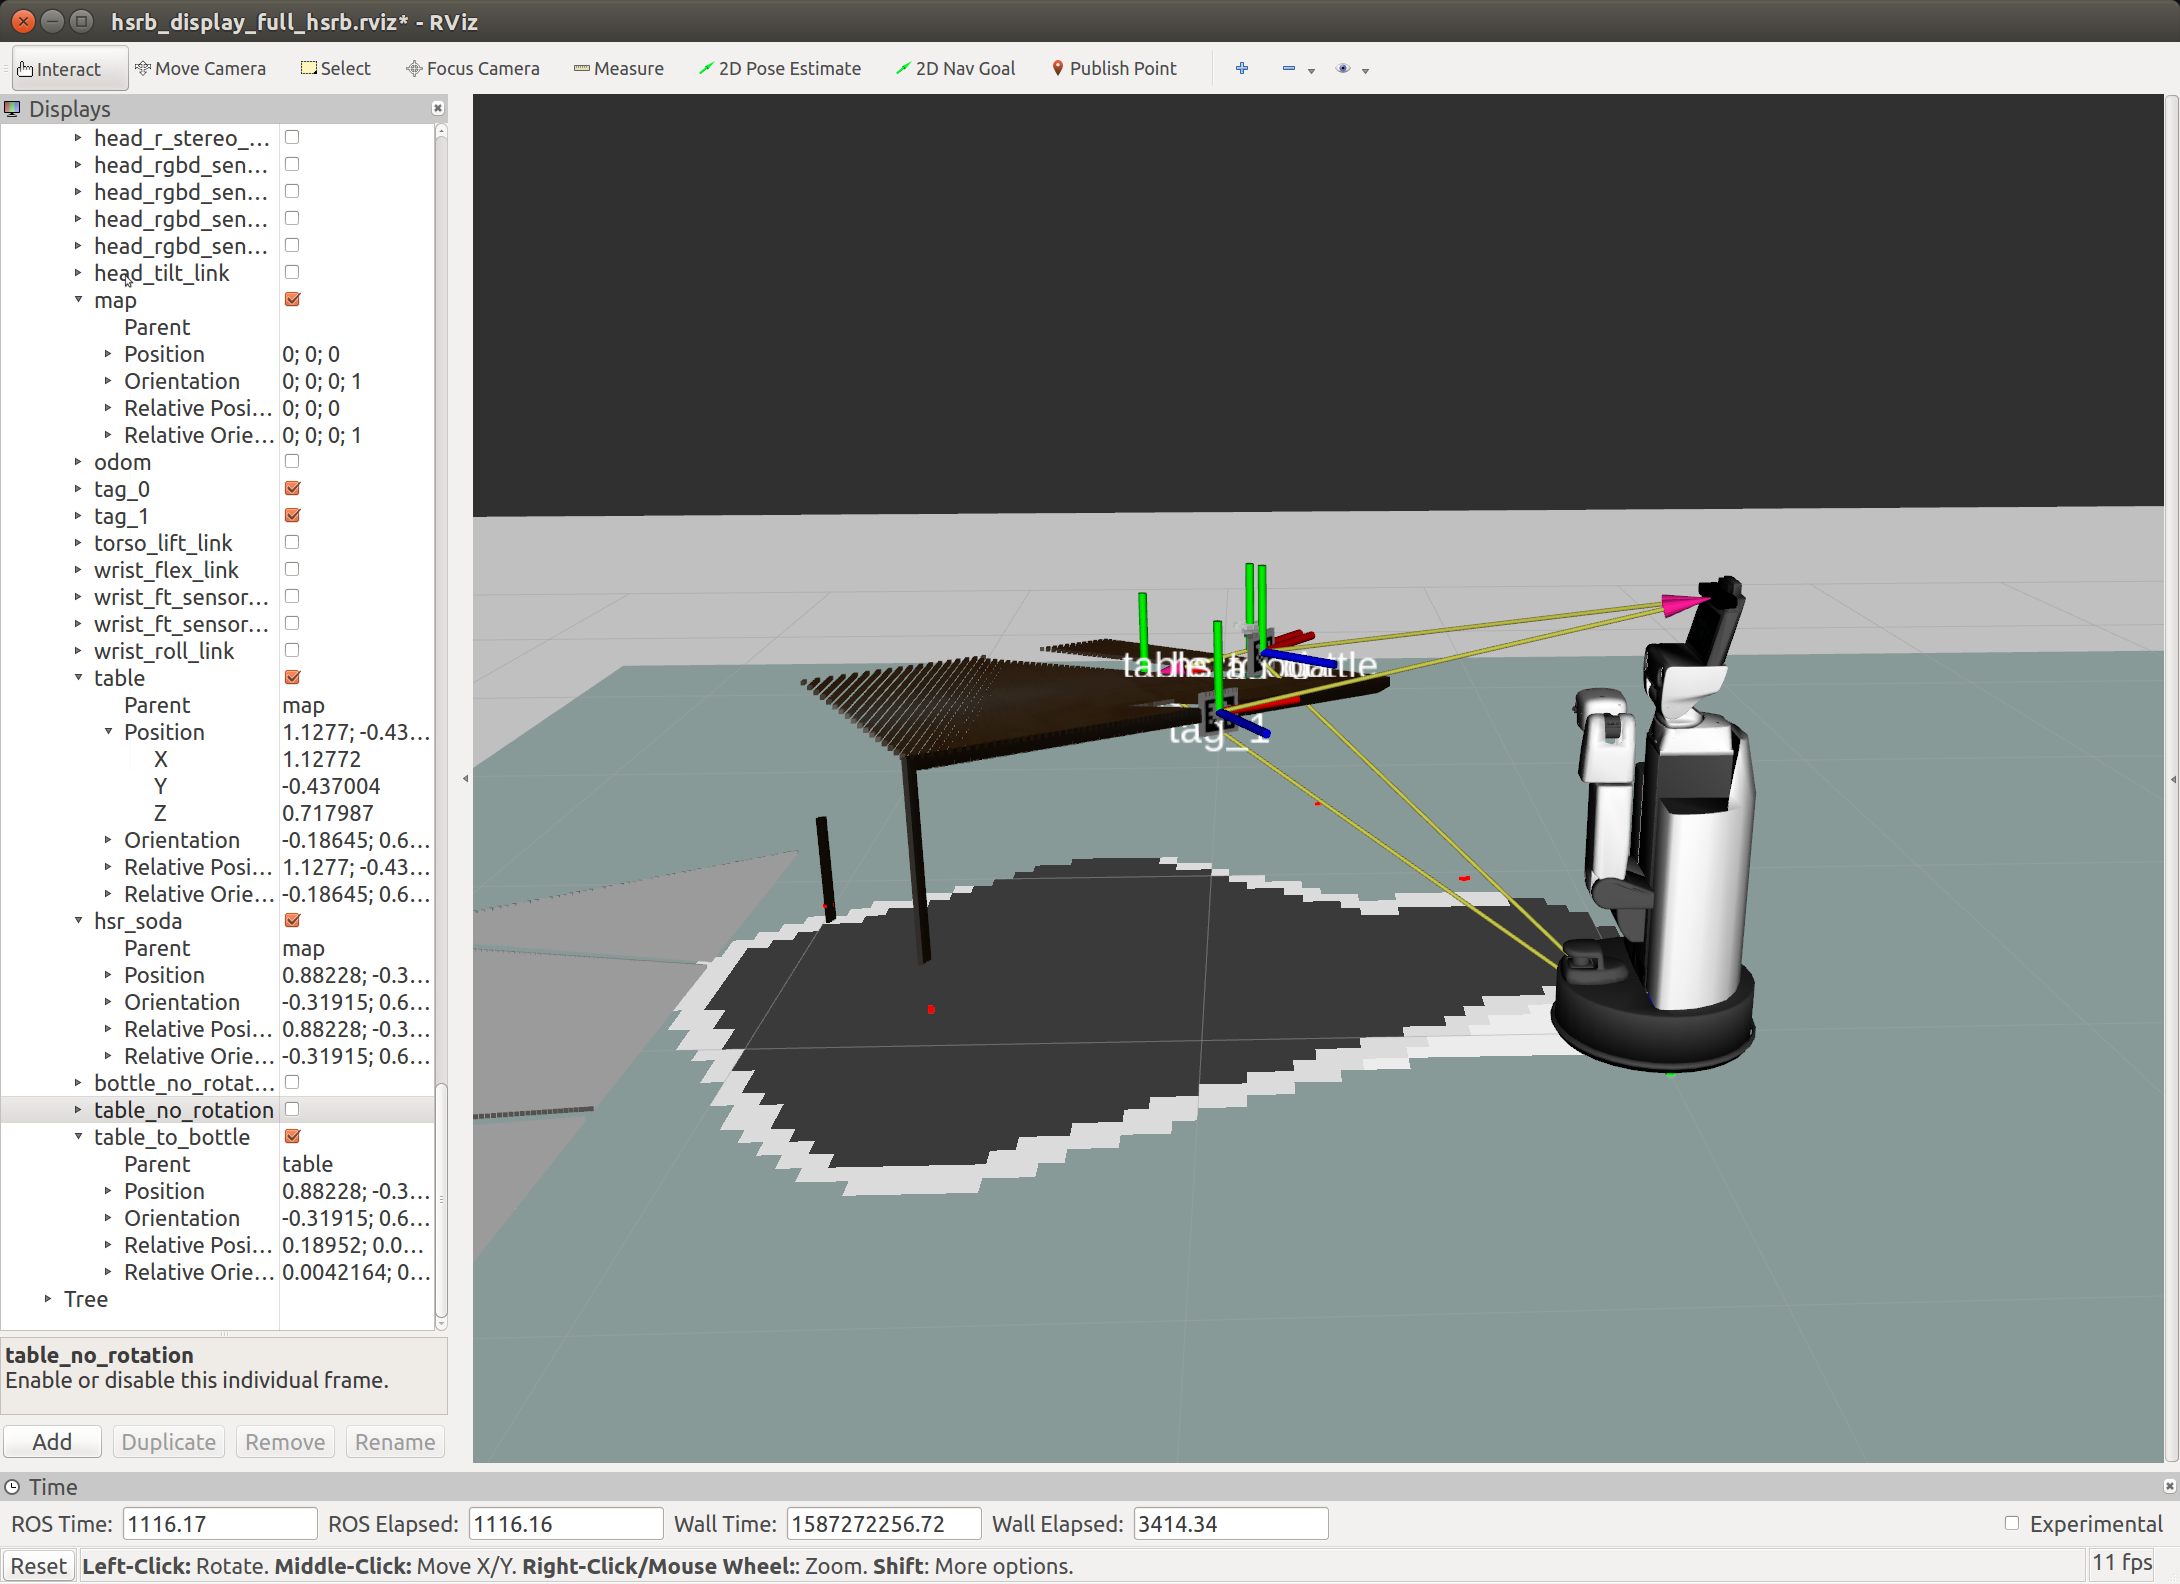
\includegraphics[width=0.45\linewidth]{2020.04.18/object_locations_rviz.png}
                    \label{fig:subfigure2}}
                    \caption{Will clean up image. (a) Gazebo visualization of world. (b) Soda can and starting pose of HSR in the extended grasping phase in the frame of the table}
                    \label{fig:figure}
                \end{figure}
                % \begin{figure}[ht][ht]
                %     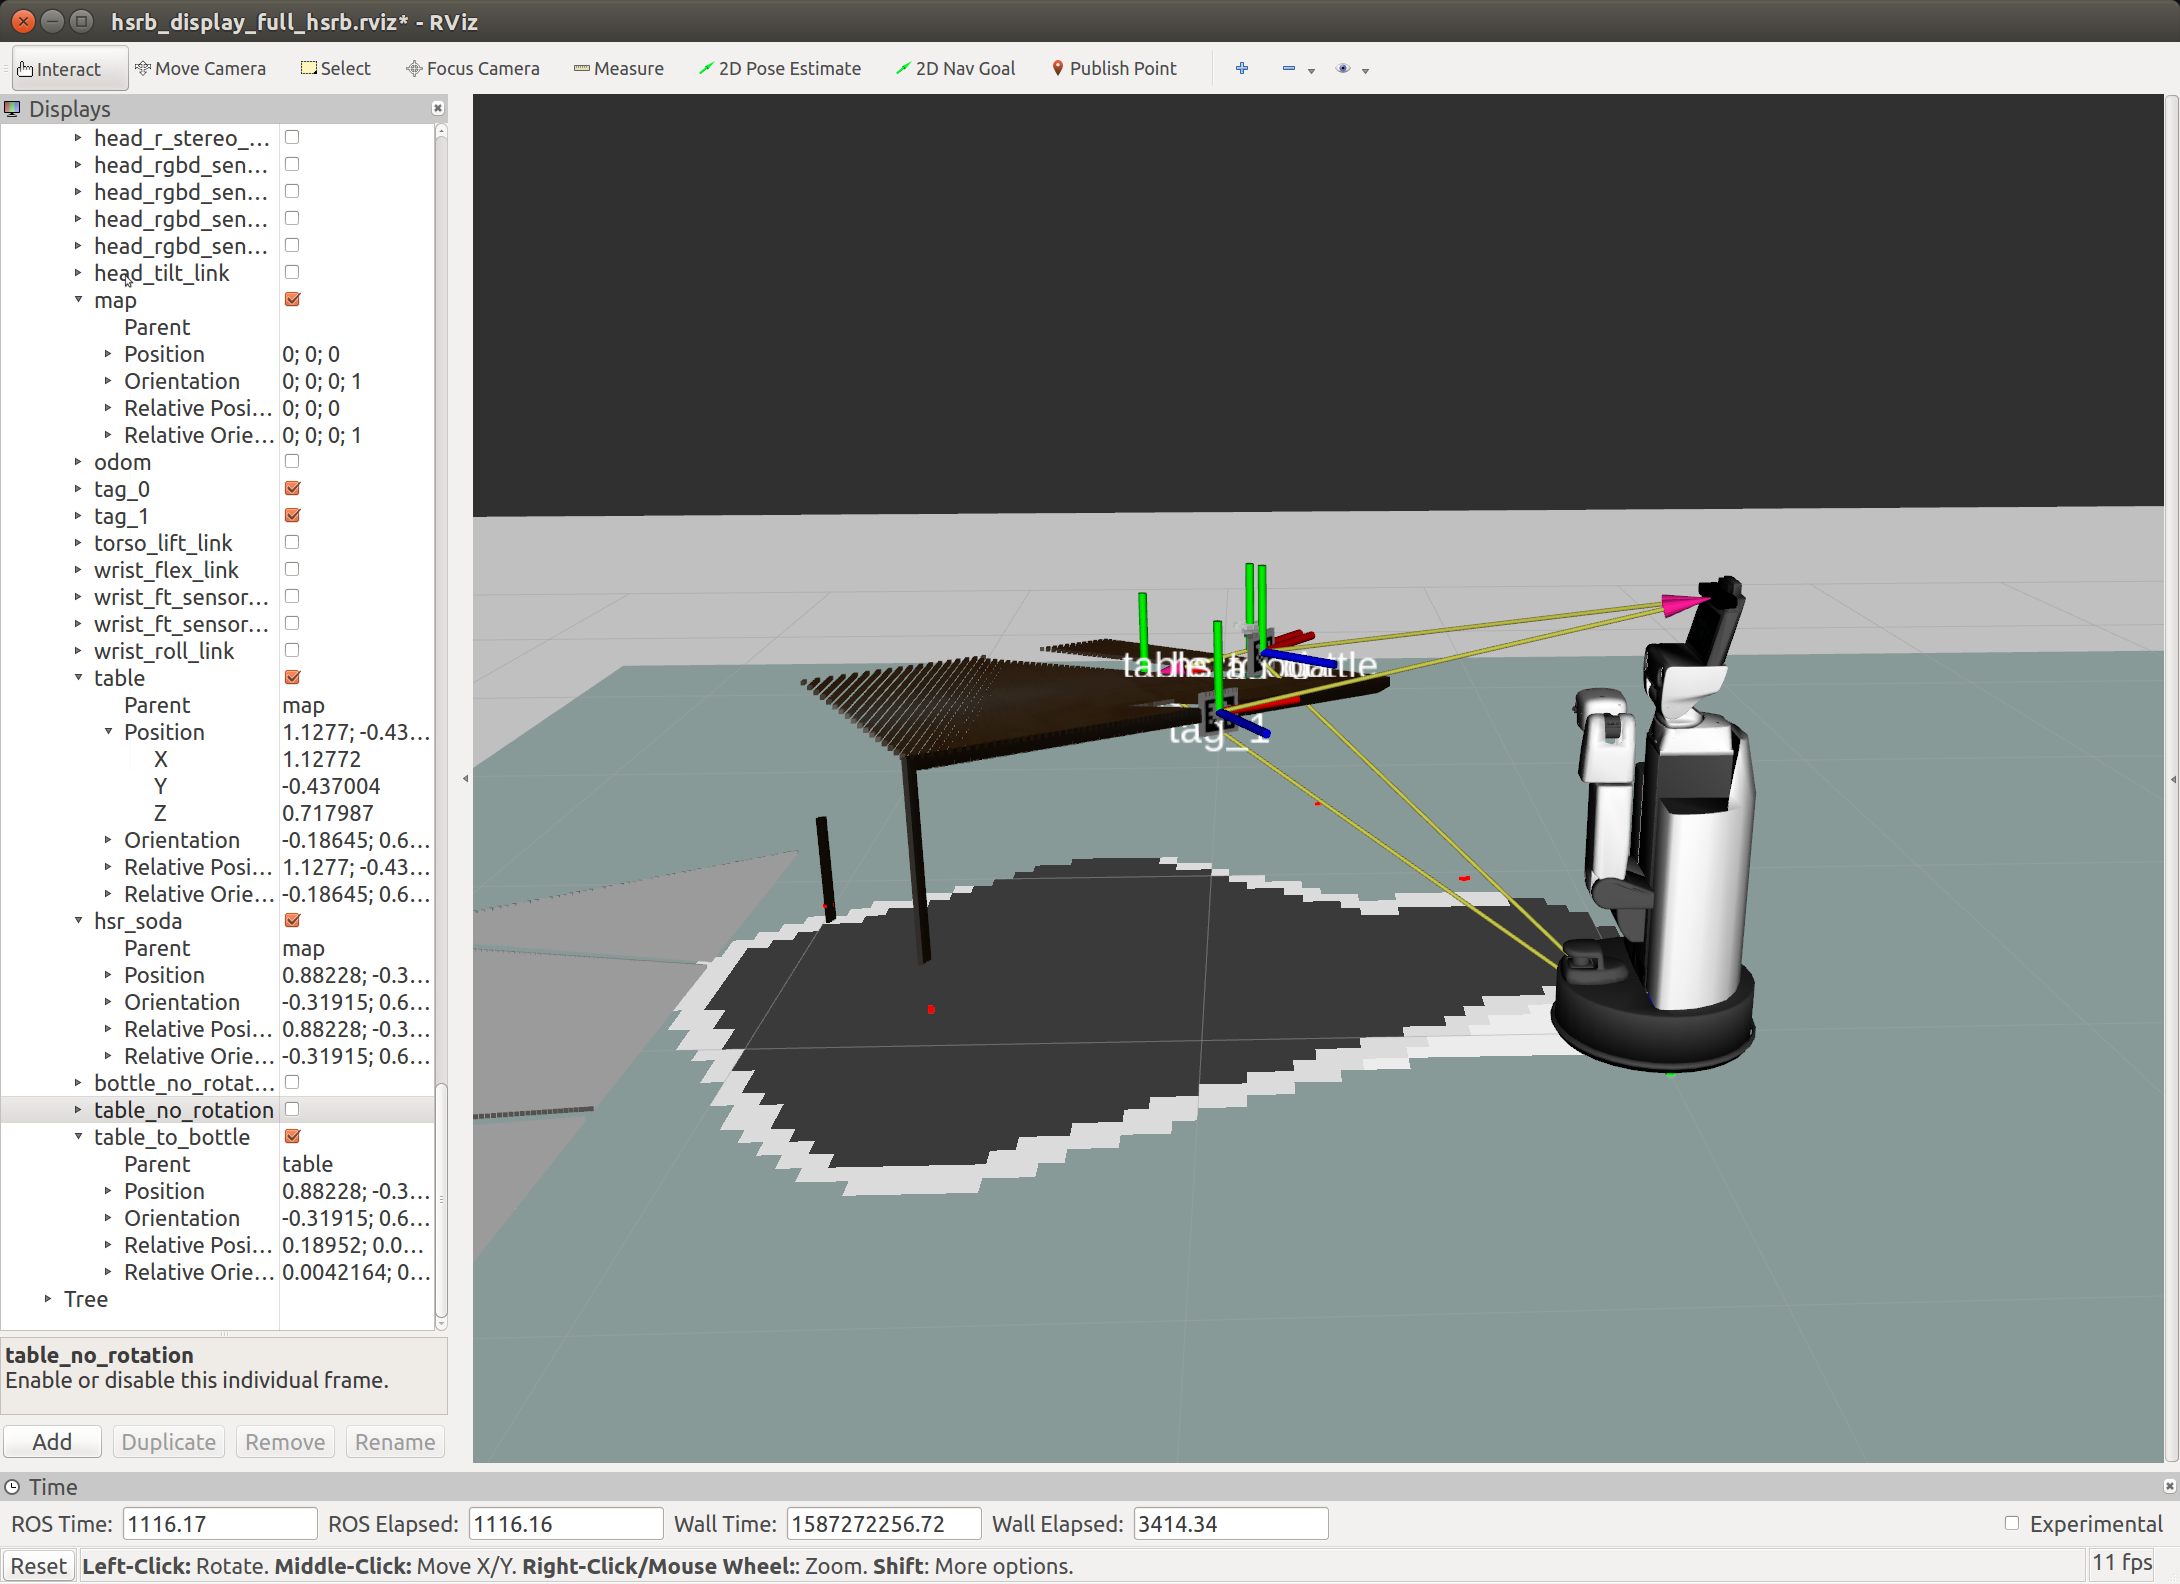
\includegraphics[width=8cm]{2020.04.18/object_locations_rviz.png}
                %     \centering
                %     \caption{[Will clean up image. Positions of target object and starting base pose for the extended grasping phase.]}
                % \end{figure}
        \newpage           
    \section{Results and Discussion}
    % 
        \begin{figure}
            \centering
            \subfigure[AICO trajectory output]{%
            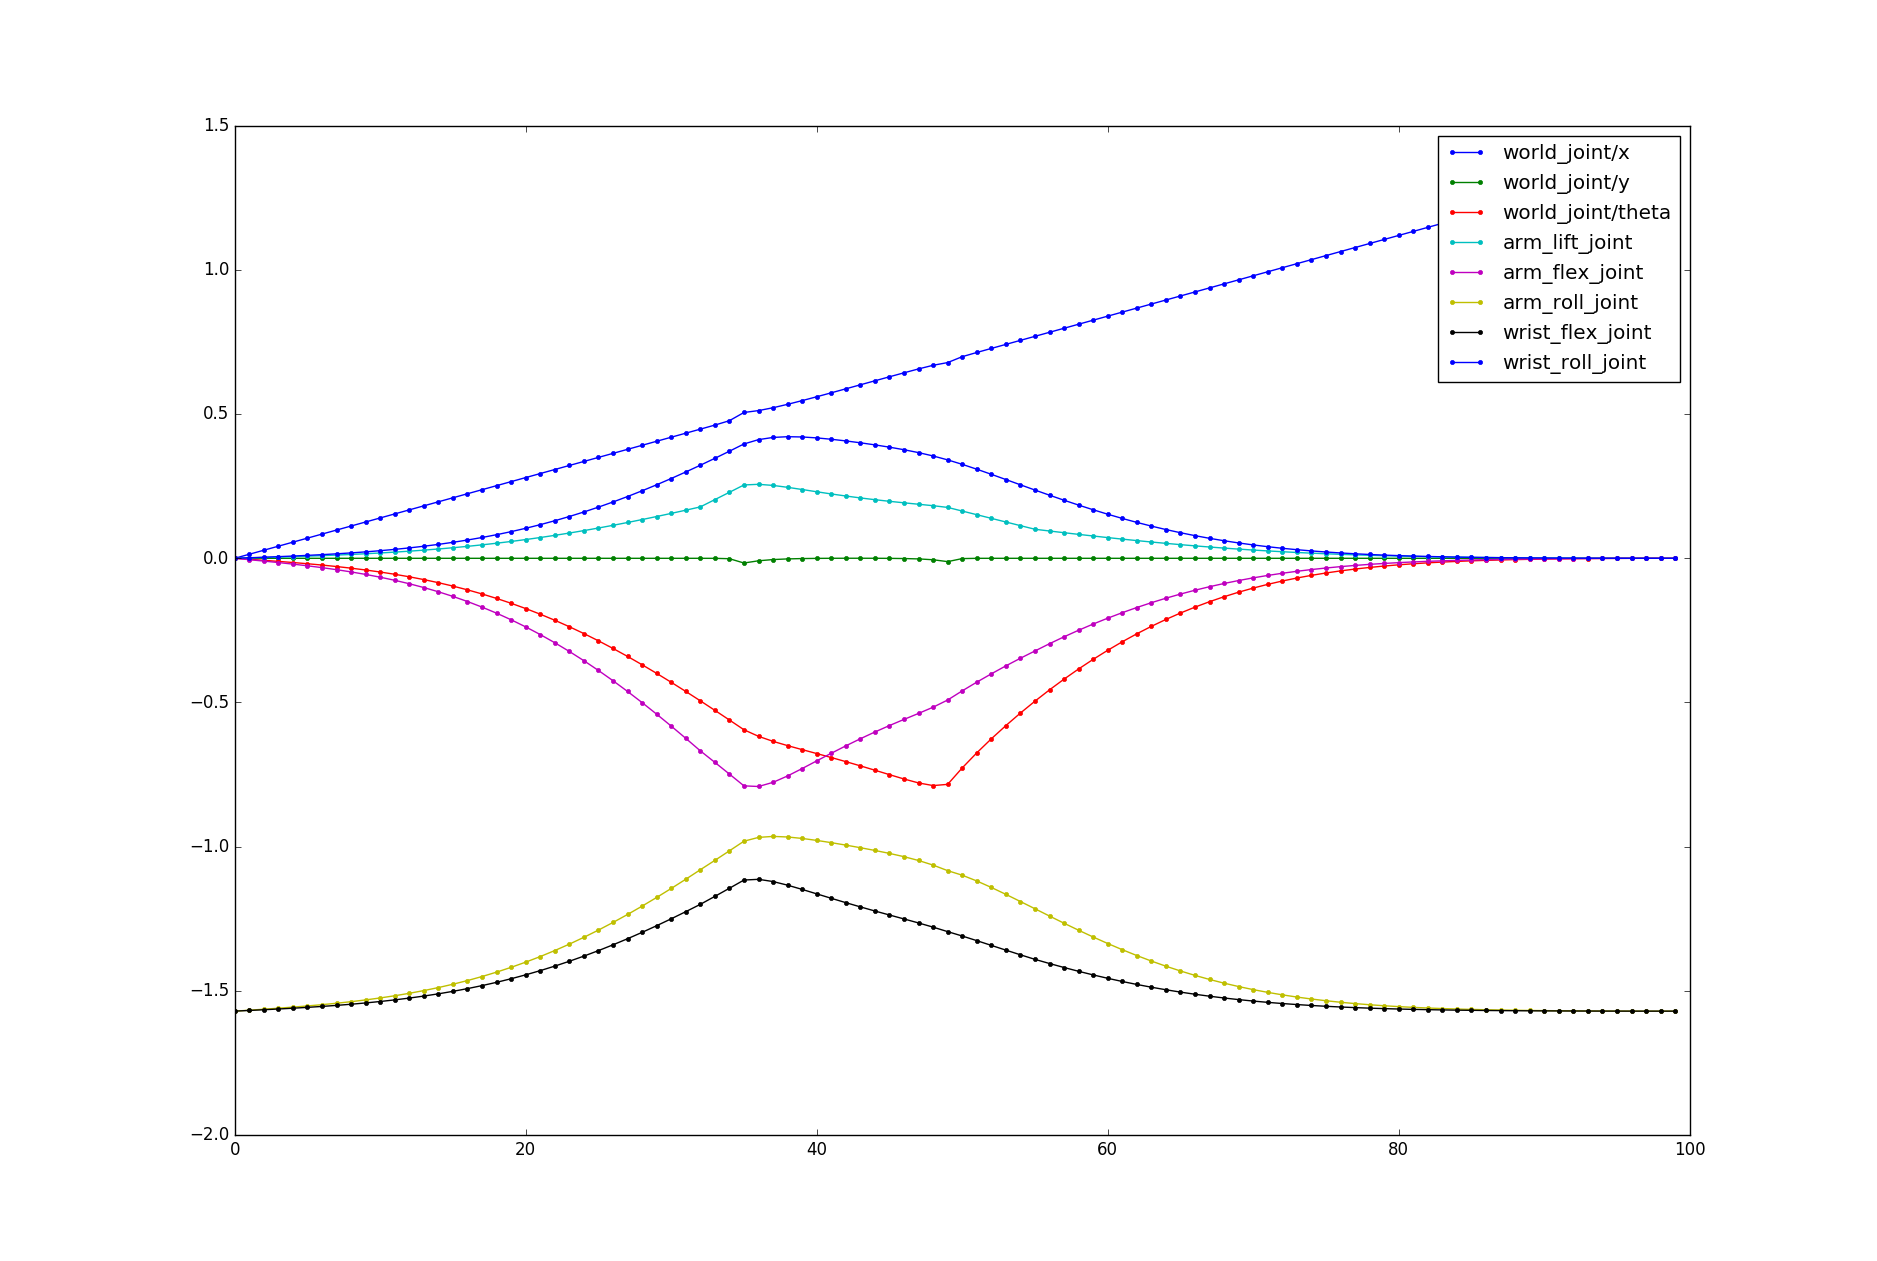
\includegraphics[width=0.75\linewidth]{2020.03.31/Solver_figure_positions.png}
            \label{fig:aicoOutput}}
            \quad
            \subfigure[Waypoint Positions]{%
            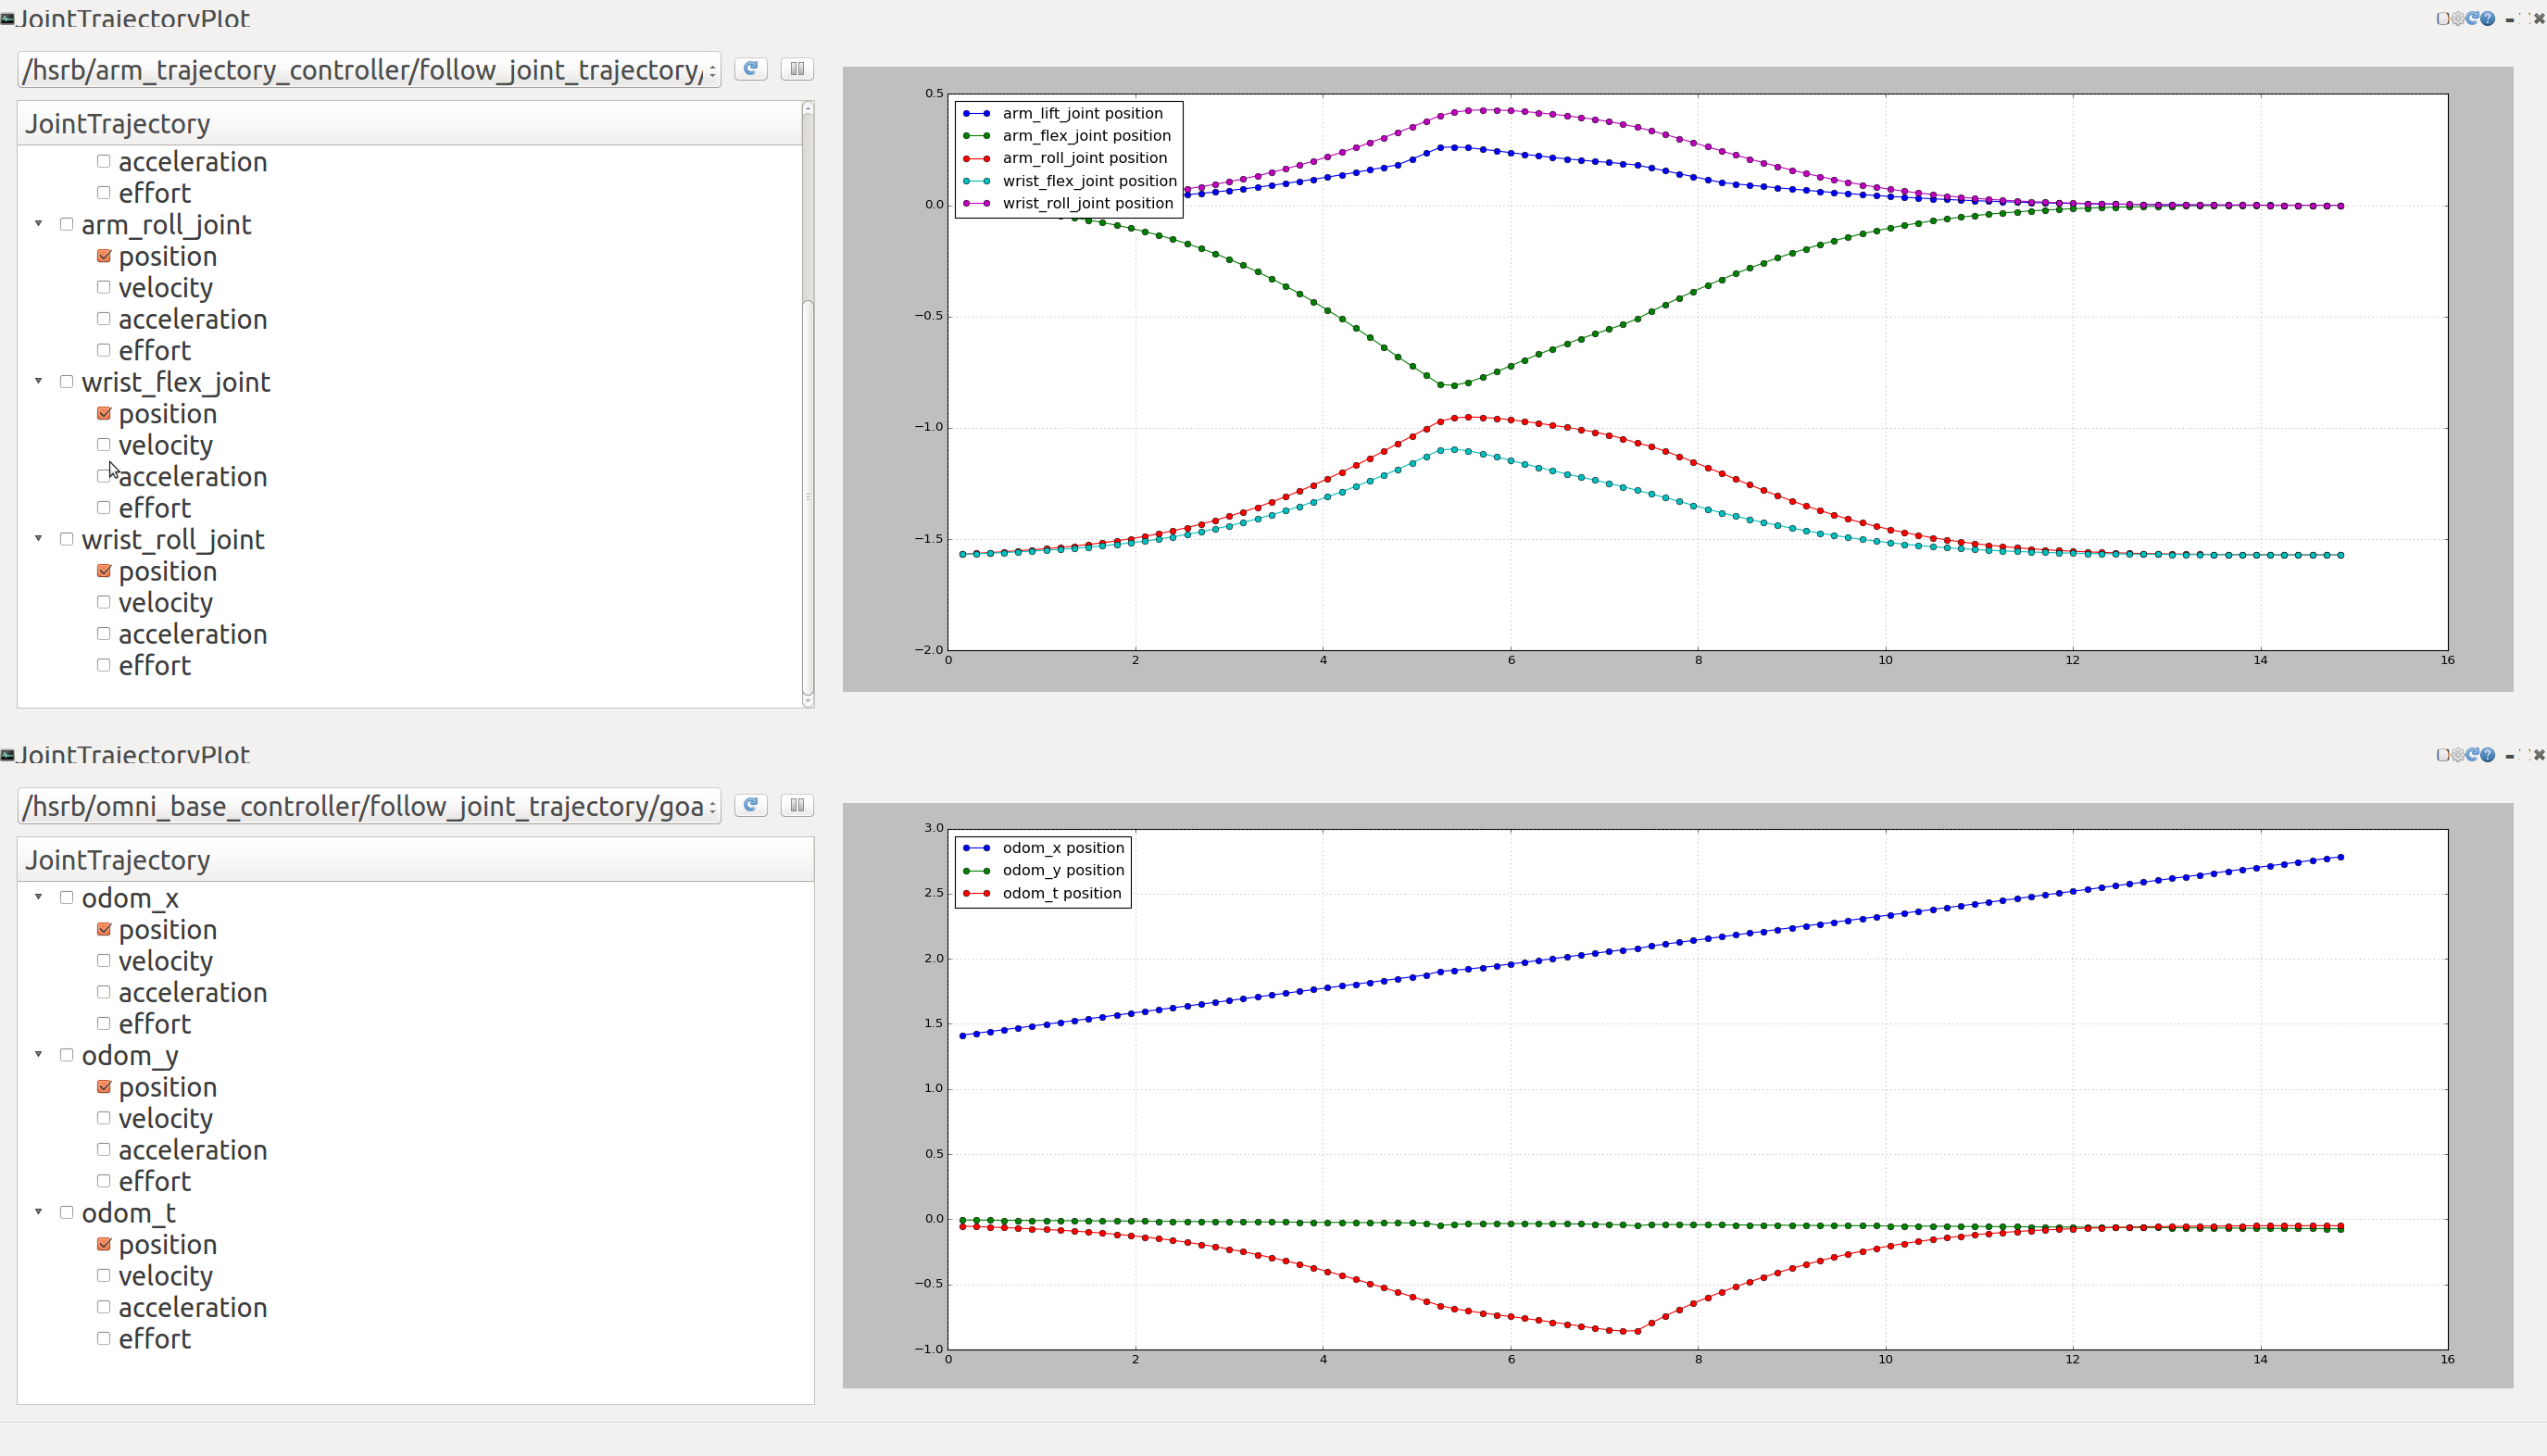
\includegraphics[width=0.45\linewidth]{2020.03.31/hsr_driveby_trajectory_position.png}
            \label{fig:idealPos}}
            \subfigure[Waypoint Velocities]{%
            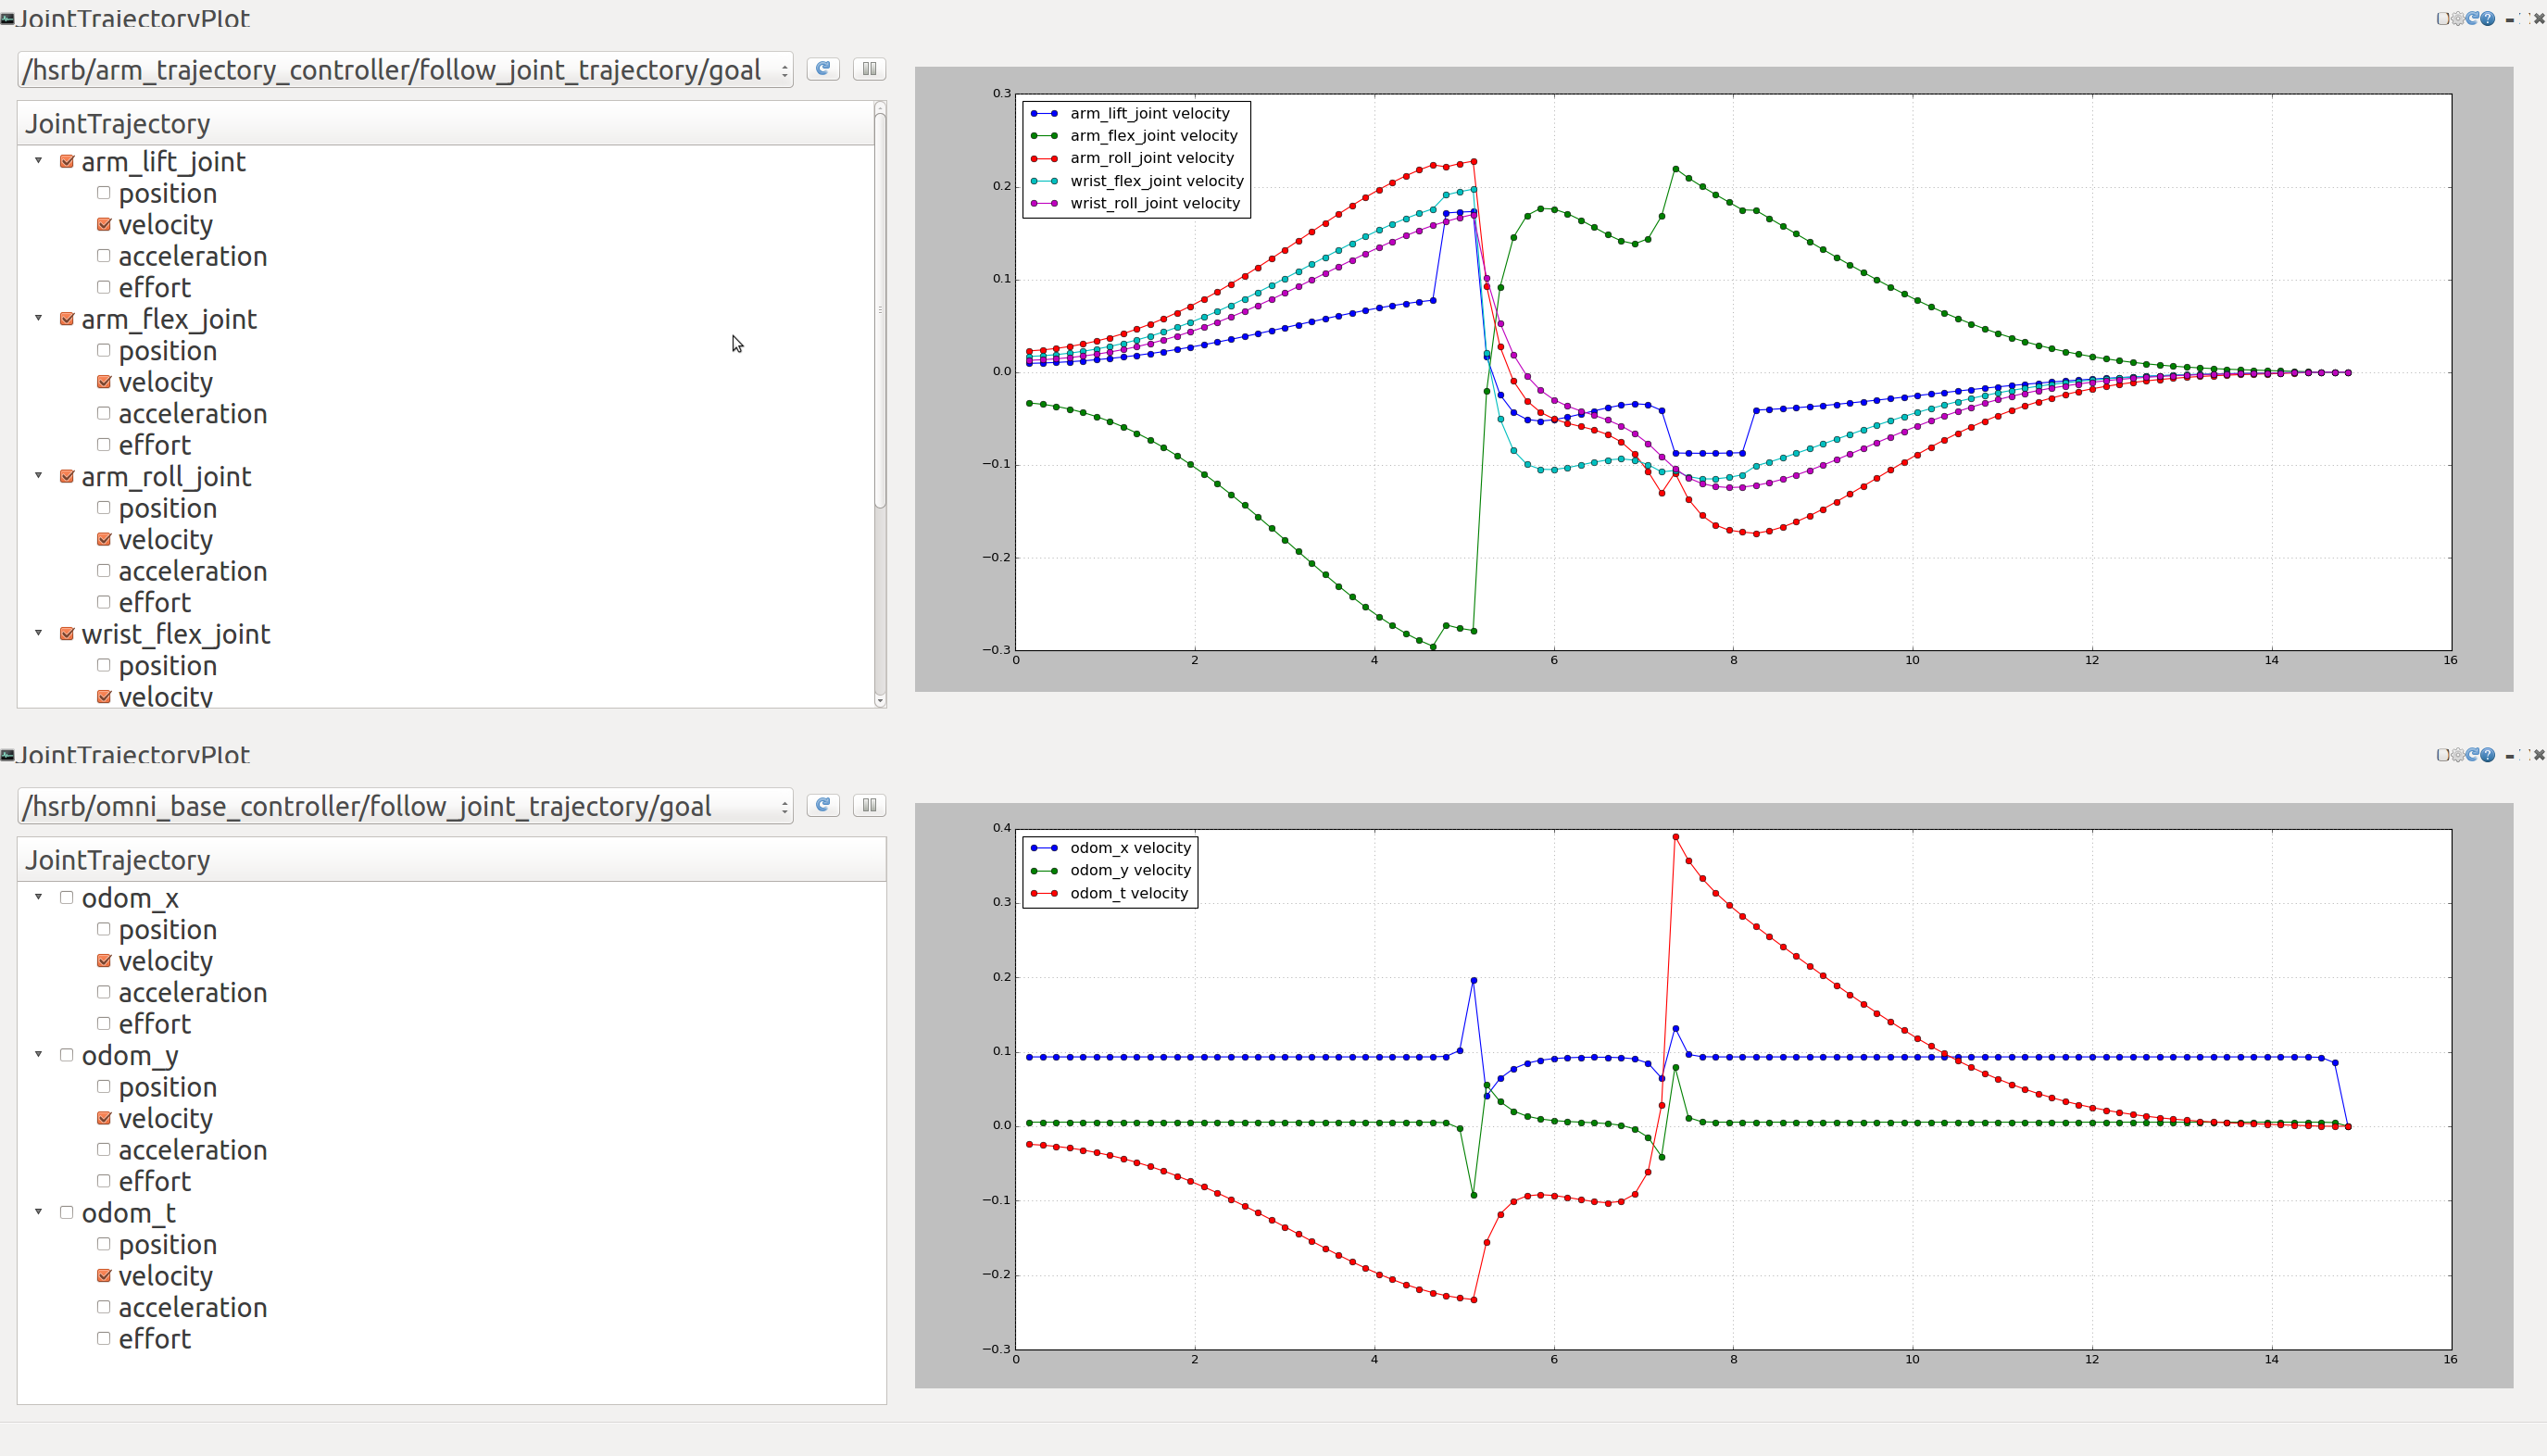
\includegraphics[width=0.45\linewidth]{2020.03.31/hsr_driveby_trajectory_velocities.png}
            \label{fig:idealVel}}
            \caption{Ideal position and velocity values at each waypoint. (a) shows the joint position values output by the AICO solver as a sanity check for (b). (c) shows a plot of joint velocities at each waypoint. Values plotted from (b) and (c) were received from messages published by /follow\_joint\_trajectory/goal topics for the HSR arm and base. This topic publishes joint\_trajectory messages at 10hz, which represent the ideal waypoints for the HSR to follow. Connections between points should be ignored since they are an artifact of plotting with RQT}
            \label{fig:IdealTraj}
        \end{figure}
        \subsection{Trajectory Analysis}
            AICO outputs a trajectory that is smooth in position \cref{fig:idealPos}, but there are no guarentees of smoothness in velocity or acceleration. For the extended grasping phase, AICO produced a trajectory with 100 waypoints. Initial trials with a timestep of 0.1 seconds for a 10 second extended grasping phase duration, found that the HSR could not reach waypoints in the alloted time and returned an error. The issue resulted from exceeding velocity constraints, specifically the arm-lift-joint (\cref{fig:arm-lift-joint}), which has a upper velocity limit of 0.2, as defined in the HSR URDF file. \cref{fig:veljoints} shows that the 15 second trajectory keeps the arm-lift-joint under the threshold.
            \iffalse Through incrementing the timestep by 0.01 seconds, the first timestep that did not result in an error was 0.15 seconds that resulted in a 15 second trajectory. \fi
            \cref{fig:IdealTraj} depicts the ideal trajectory output by the AICO solver, sent to the HSR through the joint trajectory controller.
    %  
        % \begin{figure}
        %     \centering
        %     \subfigure[Position of Arm and Base Joints]{%
        %     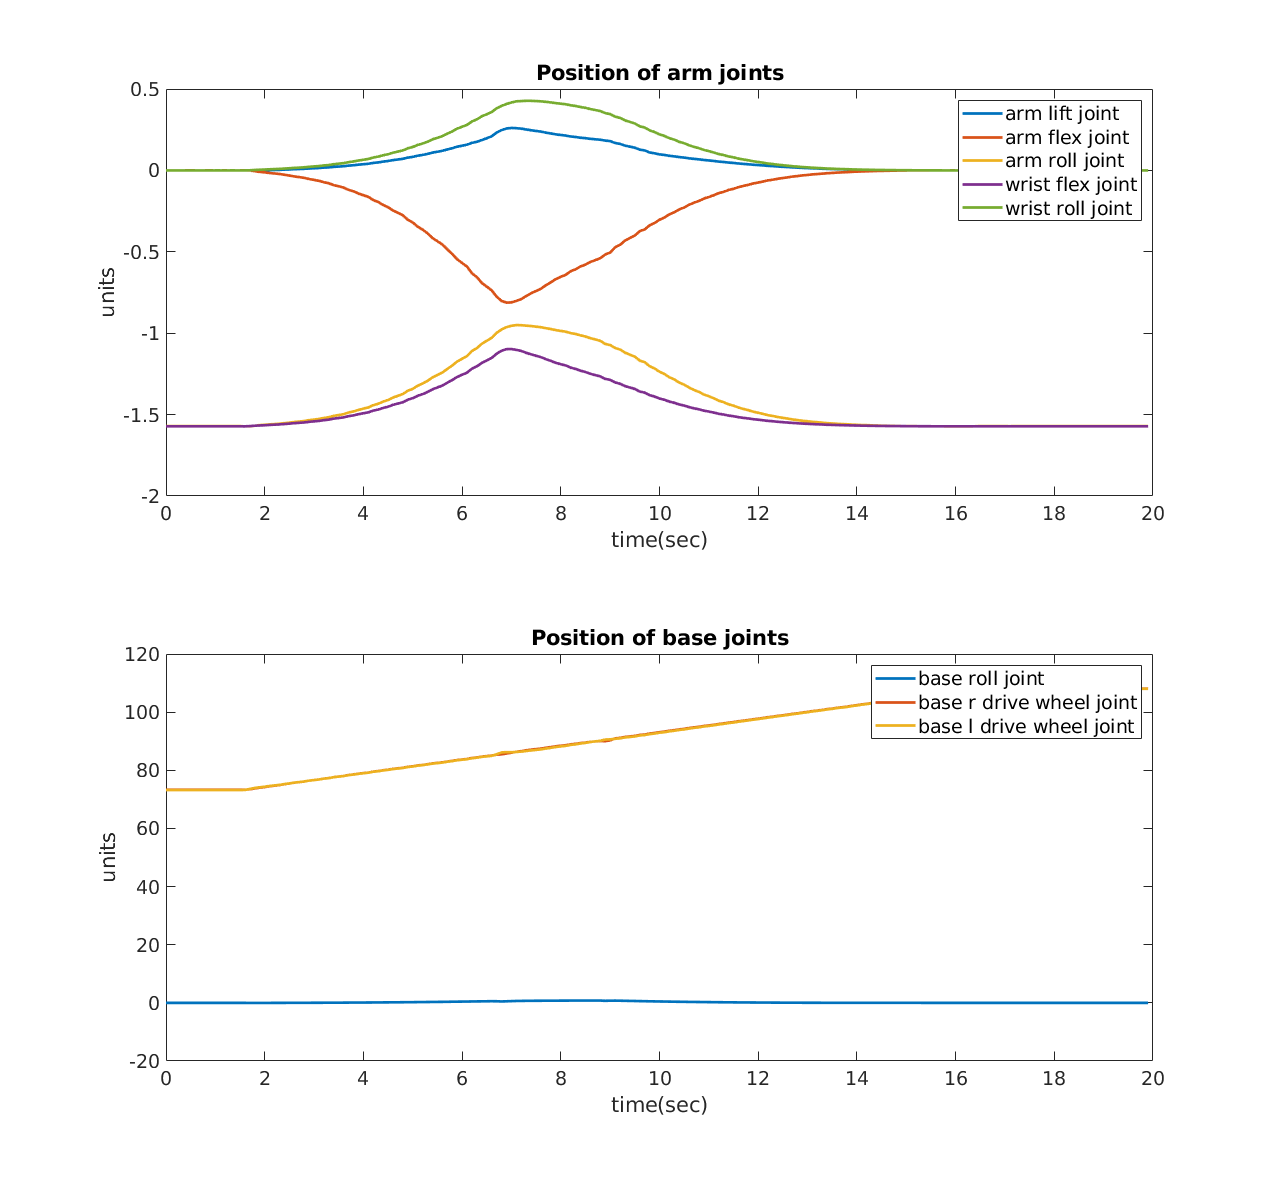
\includegraphics[width=0.50\linewidth]{2020.04.01/pos_joints.png}
        %     \label{fig:posjoints}}
        %     \quad
        %     \subfigure[Velocity of Arm and Base Joints]{%
        %     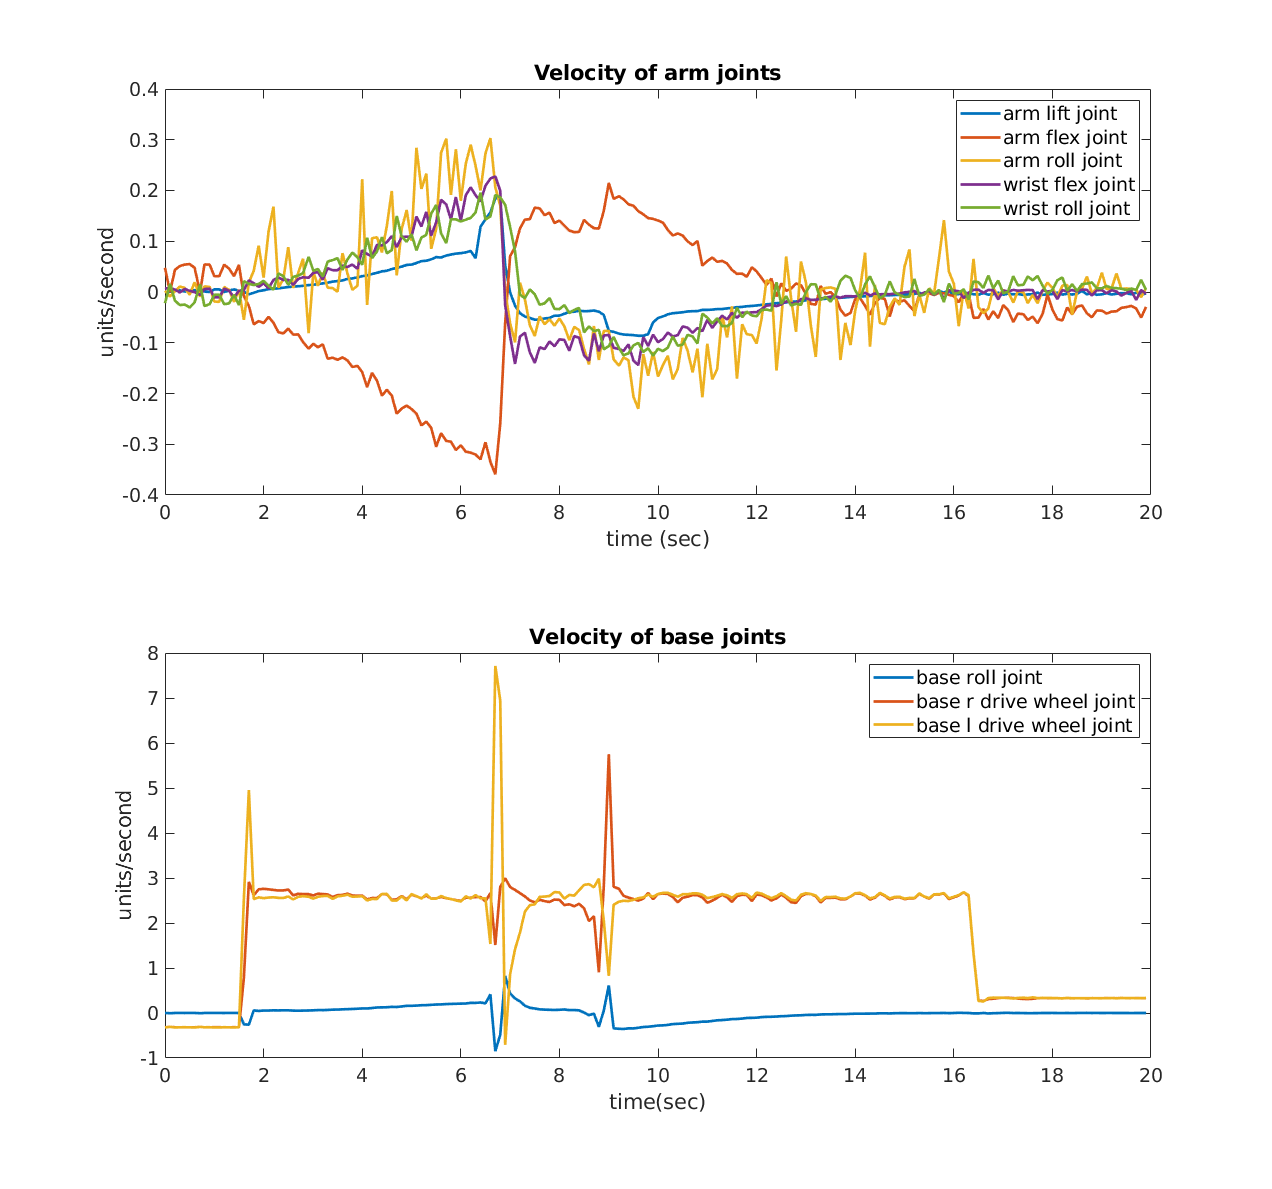
\includegraphics[width=0.50\linewidth]{2020.04.01/vel_joints.png}
        %     \label{fig:veljoints}}
        %     % \subfigure[Effort of Arm and Base Joints]{%
        %     % 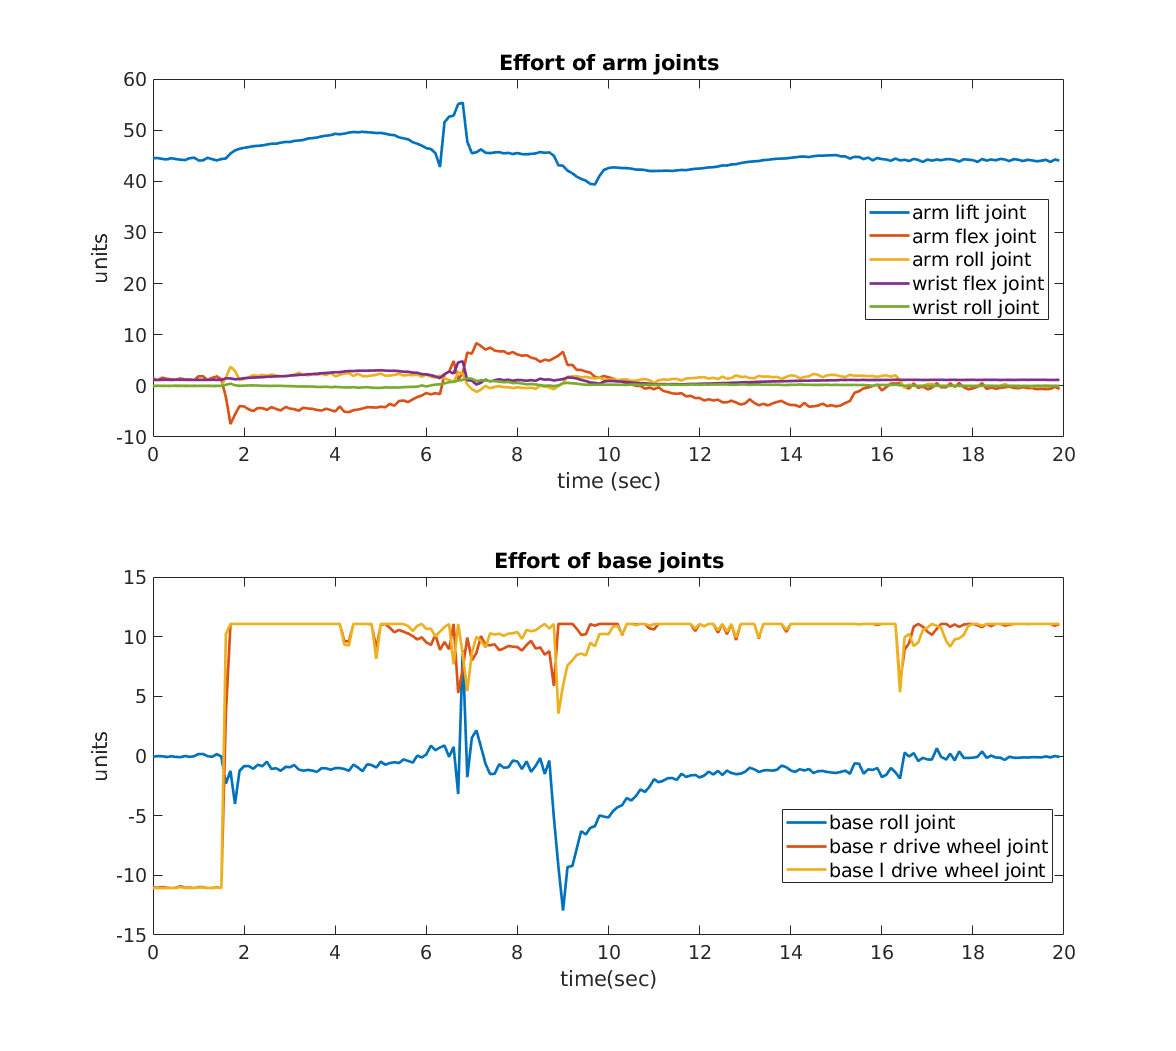
\includegraphics[width=0.50\linewidth]{2020.04.01/effort_joints.png}
        %     % \label{fig:effjoints}}
        %     \caption{Graphs of (a) Position, (b) Velocity, (c) Effort of a trajectory executed by the HSR when position and velocities are specified. Trajectory starts at ~1.5 seconds and ends at ~16.5 seconds. Plots depict trajectory messages over the /hsrb/robot\_state/joint\_states, which publishes at a rate of 10 hz. This topic Connections between points should be ignored since they are an artifact of plotting with RQT}
        %     \label{fig:first analysis}
        % \end{figure}

        \begin{figure}
            \centering
            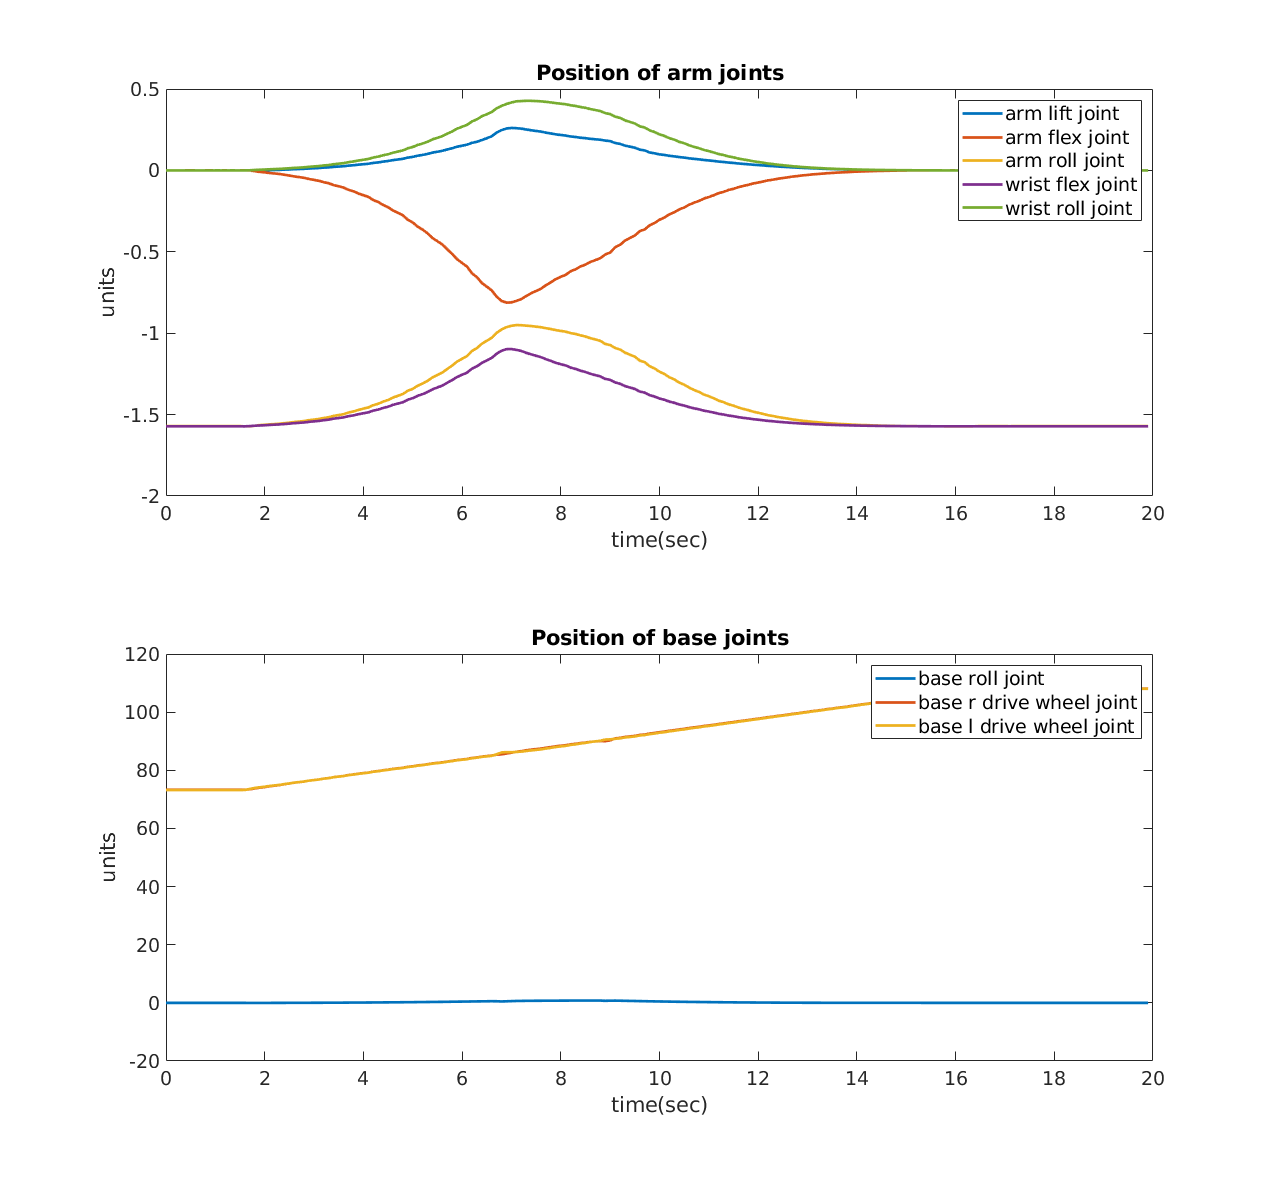
\includegraphics[width=\linewidth]{2020.04.01/pos_joints.png}
            \label{fig:posjoints}
            \caption{Graph of position of a trajectory executed by the HSR when position and velocities are specified. Trajectory starts at ~1.5 seconds and ends at ~16.5 seconds. Plots depict trajectory messages over the /hsrb/robot\_state/joint\_states, which publishes at a rate of 10 hz. This topic Connections between points should be ignored since they are an artifact of plotting with RQT}
        \end{figure}

        \begin{figure}
            \centering
            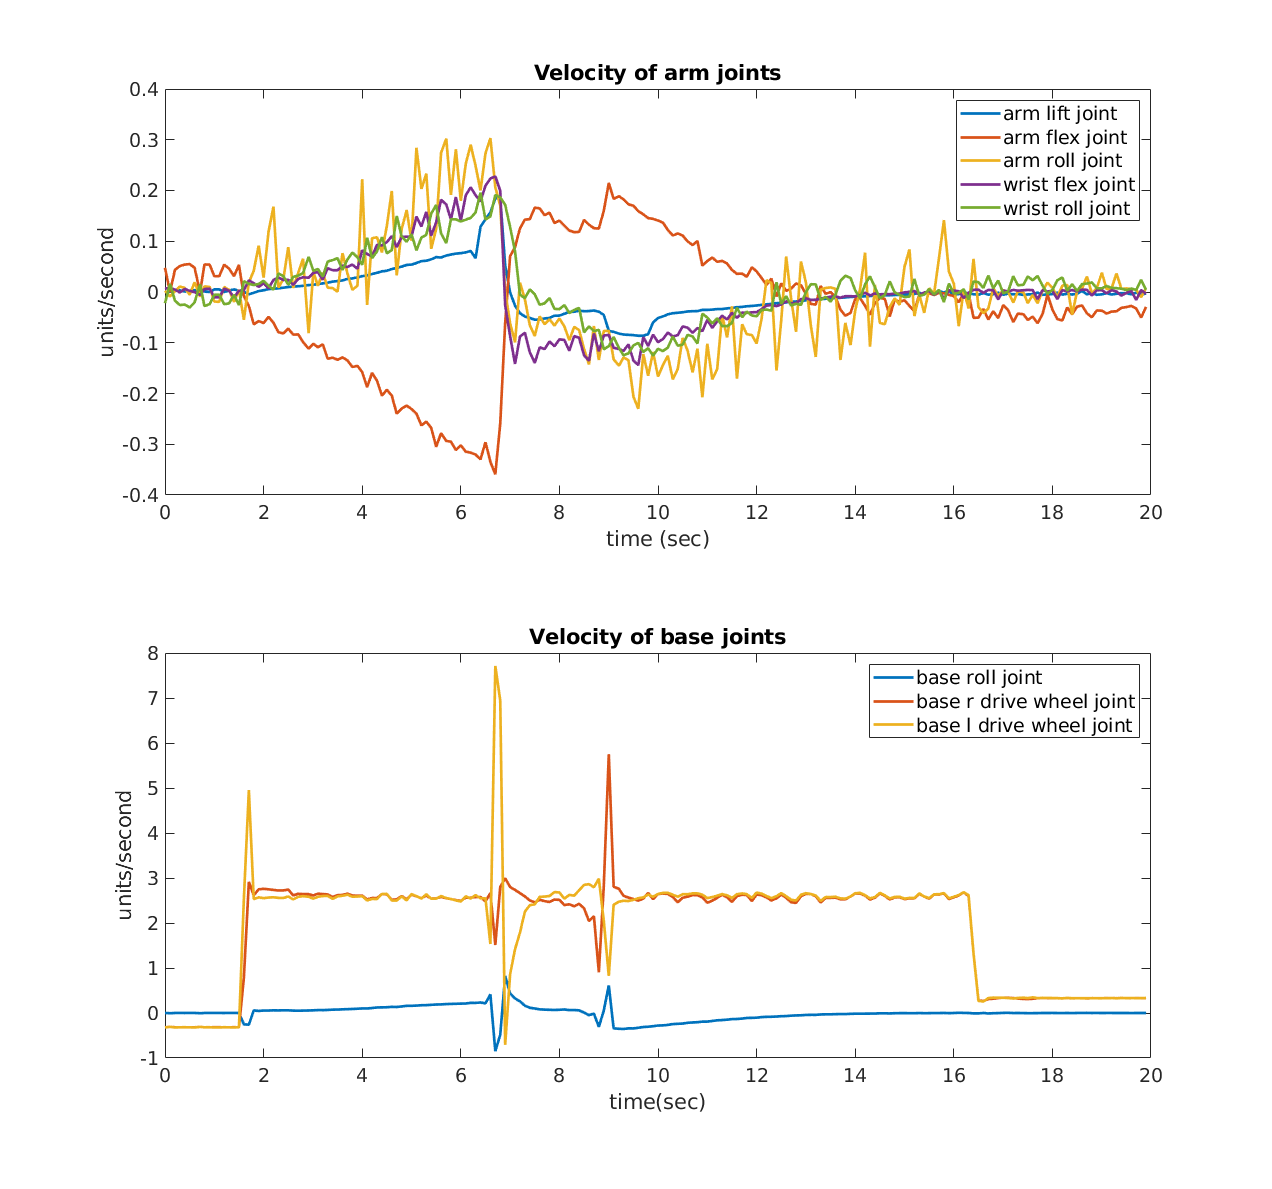
\includegraphics[width=\linewidth]{2020.04.01/vel_joints.png}
            \label{fig:veljoints}
            \caption{Graph of velocity of a trajectory executed by the HSR when position and velocities are specified. Trajectory starts at ~1.5 seconds and ends at ~16.5 seconds. Plots depict trajectory messages over the /hsrb/robot\_state/joint\_states, which publishes at a rate of 10 hz. This topic Connections between points should be ignored since they are an artifact of plotting with RQT}
        \end{figure}
        


    \subsection{Analysis of Plots}
        It is important to note that trajectory feedback measurements differ from the ideal trajectory due to noise in the robot system and also due to alterations made by the joint trajectory controller. 
        For planning the path of the base, AICO gives a trajectory with x,y coordinate positions and an angle \(\theta\) that represents the yaw of the HSR. The HSR base trajectory controller takes the x,y, \(\theta\) values and converts the values into goals for the drive wheels and the base roll joint, described in [hsr section reference]. As a result, \cref{fig:IdealTraj} base joint trajectories and labels differ from the representation in \cref{fig:posjoints}. Because base joint velocity, acceleration, and efforts are defined for the physical HSR joints, the latter labels are used for analyzing the trajectory.

        \begin{figure}
            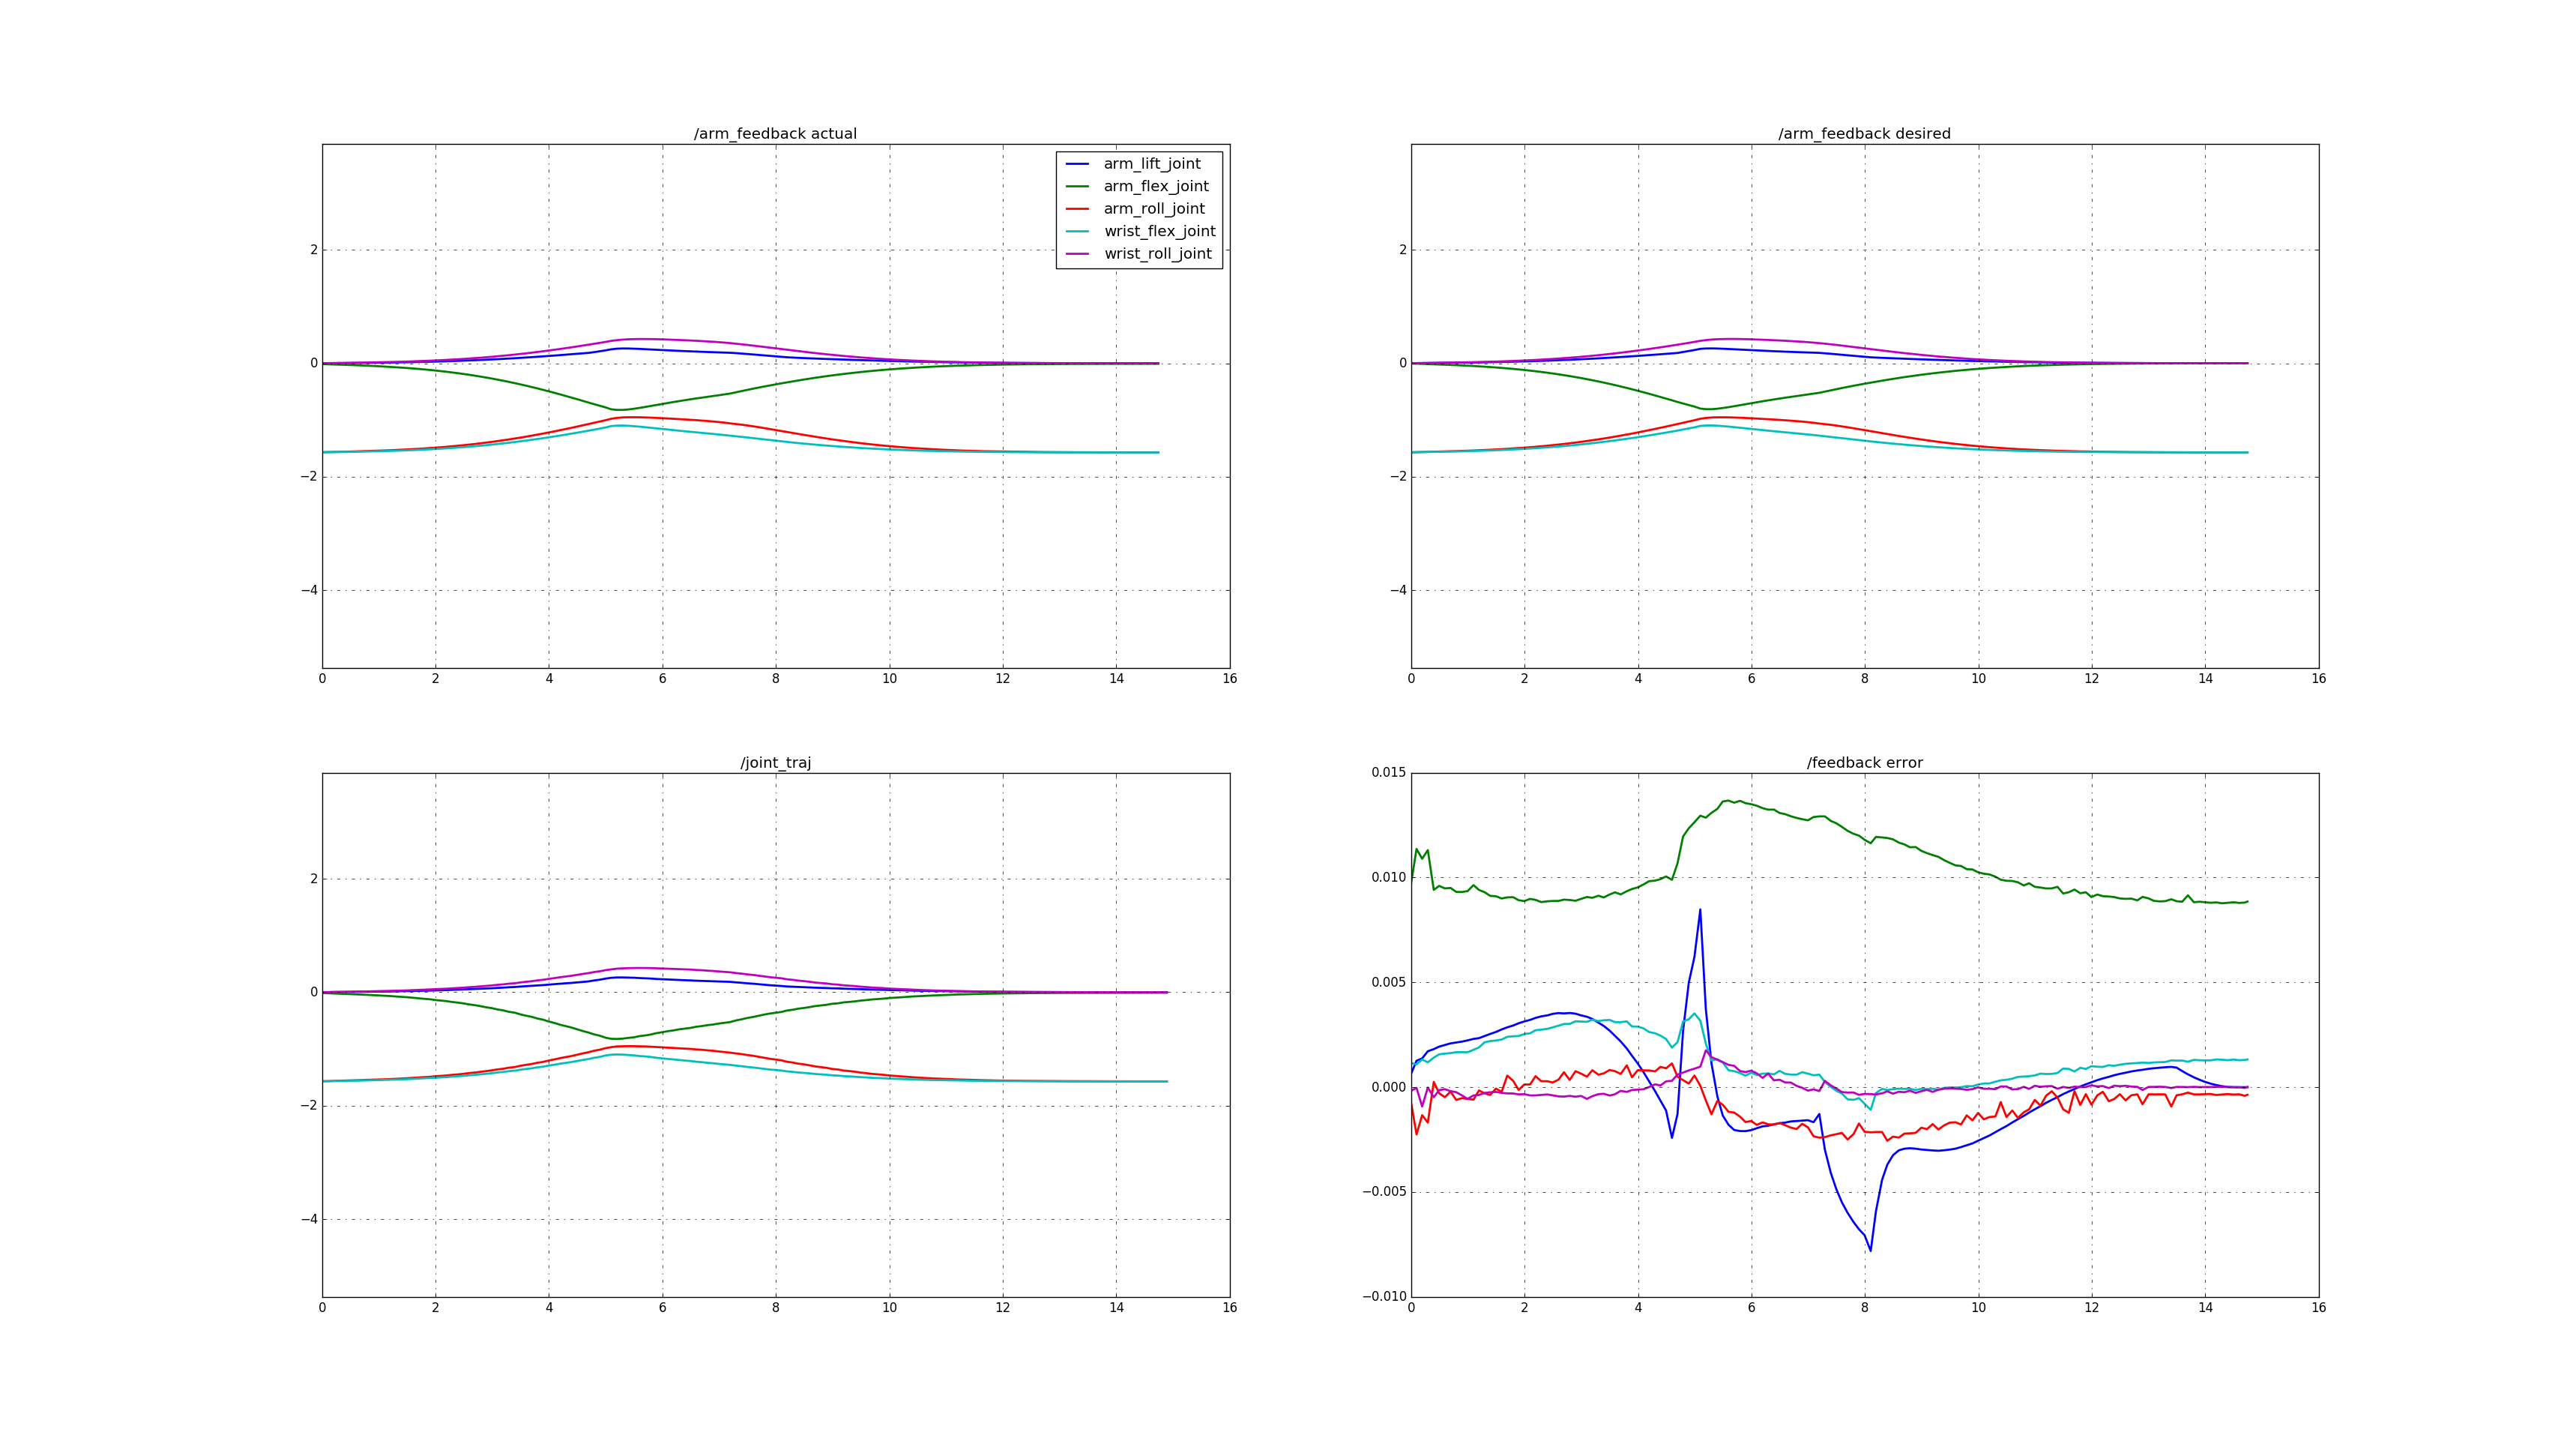
\includegraphics[width=\linewidth]{2020.04.02/positions.png}
            \centering
            \caption{All trajectories were sampled from the simulated HSR at 10 Hz. The horizontal axis has units of time in seconds and the vertical axis has units of position, meters in the case of arm lift joint and radians for all else. (top left): actual joint positions of the sim HSR arm. (top right): Desired joint positions. (bottom right): the difference between position values in measured and desired joint positions. Actual and desired values were received from a control\_msgs/FollowJointTrajectoryActionFeedback message, so the values have matching timestamps.}
            \label{fig:posAccuracy}
        \end{figure}
        % 
        \subsubsection{Joint Positions} 
            At the position level, the measured arm joint positions in \cref{fig:posjoints} match the ideal arm joint positions in \cref{fig:aicoOutput} and \cref{fig:idealPos}. \cref{fig:posAccuracy} depicts that the error in position is small in comparison to the position values. Notably, the arm flex joint and arm lift joint deviate the most from the desired values. However, considering that the 2 links are at the base of the HSR arm kinematic tree and are responsible for moving the entire weight of the arm, relatively larger deviations are acceptable.
            \par Further, a visual check of the trajectory in Rviz and Gazebo confirms that the error in joint positions did not significantly impact the trajectory since the HSR successfully grasped the soda can during the extended grasping phase and reached the end pose. \par From \cref{fig:posjoints} it appears that the HSR base follows the linear drive-by trajectory very closely, with slight deviations at the start and end of the sub-grasping phase between 7 and 9 seconds in \cref{fig:posjoints} indicated by small disturbances in base drive joint plots. These abrupt changes in position are due to task maps becoming active during the sub-grasping phase. The base roll joint plot does not accurately capture the change in HSR body orientation, due to the large values in the drive wheel joint position. [insert new plots without resets and separate roll joint from drive joints].
        % 
            \par The HSR accomplished the grasping phase of the drive-by pick-and-place problem in simulation. Although the joint position limits for the simulated HSR are slightly greater than the values given for the actual robot, the joint positions in the trajectory simulation fall below both boundaries as a result of the joint limit task map. [insert chart of joint limits in hsr manual compared to limits in urdf file.]
        % 
        \begin{figure}
            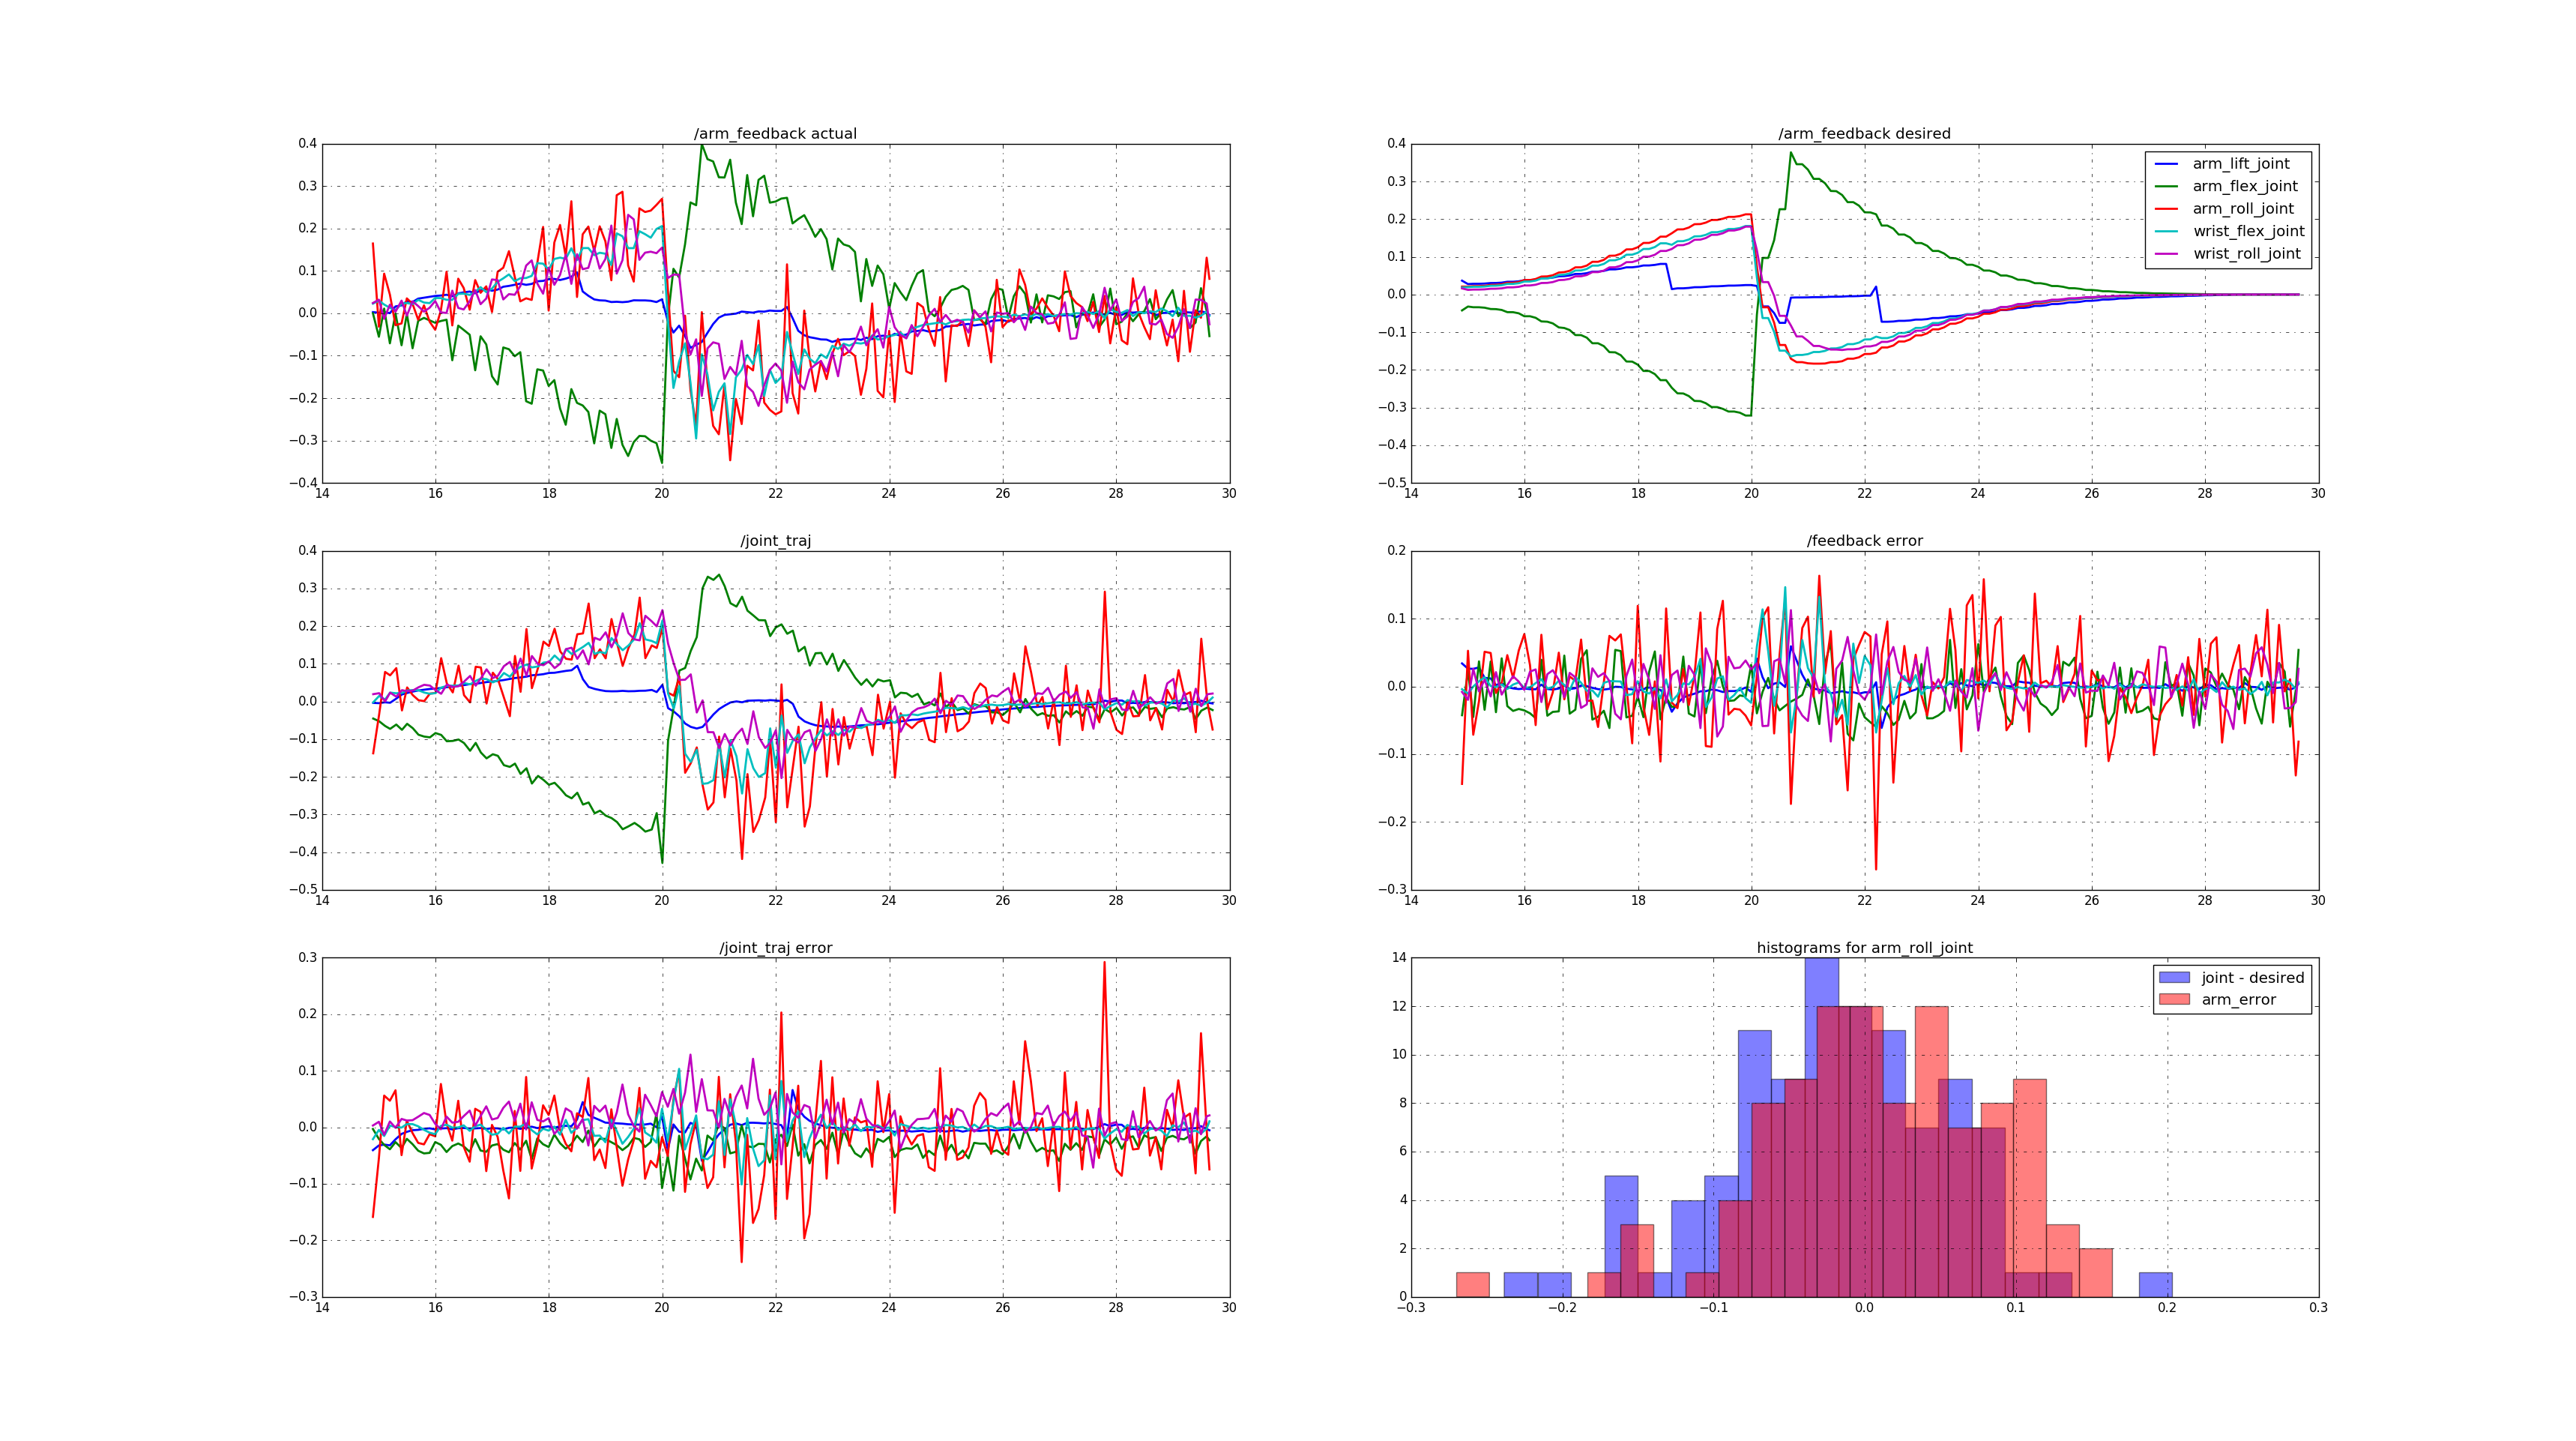
\includegraphics[width=\linewidth]{2020.04.03/t8/figure_1_first_100_points_20_bins_trial6.png}
            \centering
            \caption{For non-histogram plots, the horizontal axis has units of seconds and the vertical axis has units of velocity. (Top row): Measured and desired joint velocity values for the simulated HSR. Corresponding points have matching timestamps. (Middle left): Velocity measurements sampled from the simulated HSR trajectory. Timestamps do not exactly match those of the desired plot. (Middle Right): Plot of difference between time-synchronized joint velocity measurements. (Bottom Left): Plot of difference between velocity measurements of /joint\_traj and desired. (Bottom right): histogram of velocity error values for the arm roll joint.}
            \label{fig:velocityAccuracy}
        \end{figure}
        % 
        \begin{figure}[ht]
            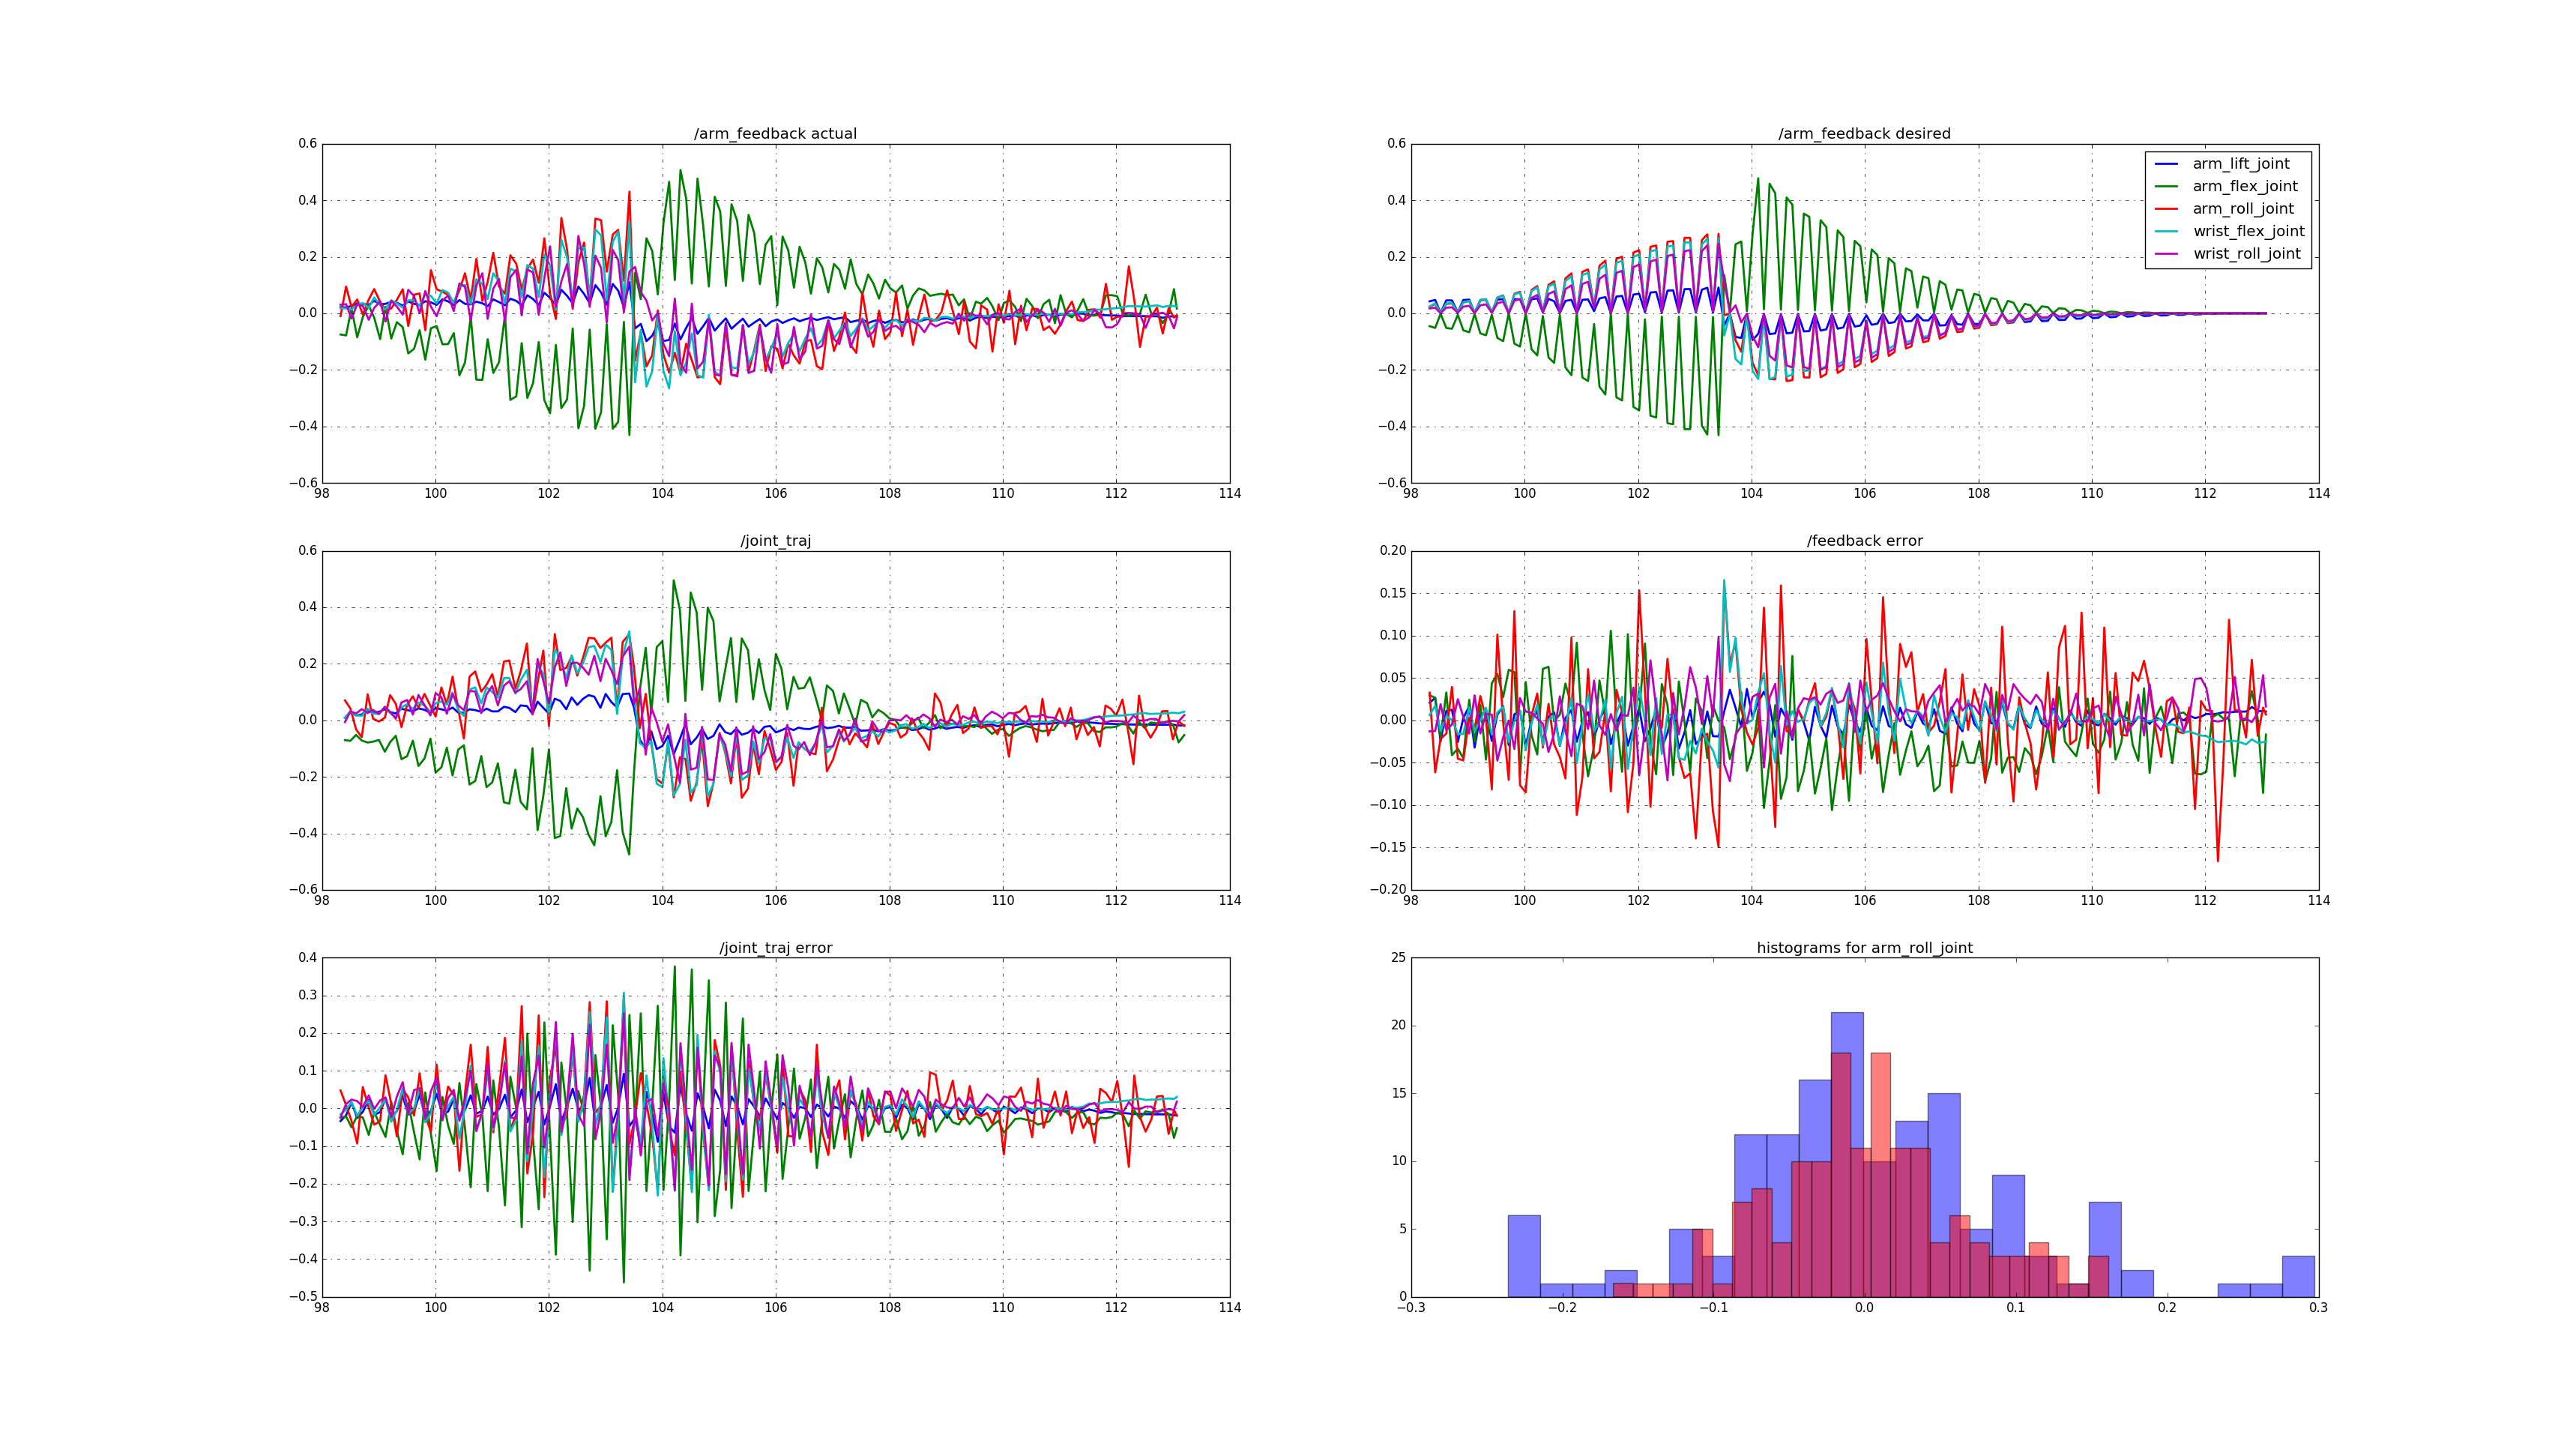
\includegraphics[width=\linewidth]{2020.04.07/arm_vel_goals_set_to_zero.png}
            \centering
            \caption{Plots in a similar order to those in \cref{fig:velocityAccuracy}. Joint velocities were set to zero at each trajectory waypoint.}
            \label{fig:velocityZero}
        \end{figure}
        % 
        \subsubsection{Joint Velocities}
            [insert table of joint velocity limits]
            The joint velocity measurements fall within velocity limits for both the physical robot and simulated robot. [reference limit table]. 
            \par One issue is the prevalence of periodic perturbations in the desired arm joint velocities in \cref{fig:velocityAccuracy} that are not present in the desired velocity plot in \cref{fig:idealVel}. The joint velocity values in \cref{fig:idealVel} represent the velocity goal at each trajectory waypoint and are obtained from differentiating the joint position trajectory generated by the AICO solver. The perturbations in \cref{fig:velocityAccuracy} result from interpolation performed by the HSR trajectory controller that ensures smoothness in velocity.

            \par Another glaring issue is the significant noise in the measured velocities in \cref{fig:velocityAccuracy}. The histogram plot in \cref{fig:velocityAccuracy} appears to be zero-mean and roughly gaussian. Thus, three possibilities were proposed to explain the disturbances.
            \begin{itemize}
                \item 1. The deviations are due to noise in measurement.
                \item 2. The deviations are due to noise in the simulated joint velocity.
                \item 3. The velocity is attempting to return to zero at each time step, resulting in large disturbances.
            \end{itemize}

            \cref{fig:velocityZero} demonstrates the effect of setting the velocity at each waypoint to zero. The perturbations are much more ordered than in the case of \cref{fig:velocityAccuracy}, and the desired joint velocity plot would show more extreme rapid changes in velocity. This rules out explanation 3. 

            \par Since the physics are simulated, explanations 1 and 2 become indistinguishable unless noise is specifically added after a measurement is taken. Conditions relating to noise must be described in the HSR urdf. Checking the urdf file yields Gaussian noise tags for joints in the head and base segments of the HSR, but none specified for arm joints. However, a damping parameter in the dynamics tag is specified for each arm joint. The damping parameter is set to 1.0 for all arm joints aside from the arm roll joint which has a damping parameter of 0.1. The dynamics tag specifies physical properties of joints and the damping parameter specifically controls the decay of velocity. The fact that the damping parameter of the arm roll joint is lower partially explains the higher amounts of noise in \cref{fig:velocityAccuracy}.

        \subsubsection{Joint Acceleration}
            % [Need to make new plots and adjust the trajectory to reduce the exceeding of acceleration constraints]
            % [Caveat= Velocity is noisy so acceleration calculation is somewhat unreliable.]
            Since the joint velocity values for the drive-by pick-and-place trajectory are not smooth, the joint acceleration plot exhibits high peaks that correspond with sharp velocity changes. \cref{fig:accelerations_ideal} depicts the desired acceleration for the trajectory from the AICO solver. The normalized desired acceleration plot shows that acceleration limits are exceeded for the arm-lift and arm-flex joints at approximately 5 seconds. The two peaks coincide with the start and end of the end-effector positioning and axis alignment tasks. This indicates that further modifications to the drive-by pick-and-place problem targets and costs would be required to drastically decrease the magnitude of the acceleration peaks. In addition, reducing the joint velocities by executing the trajectory over a longer duration of time would also contribute to decreasing the joint acceleration values.
            \par The acceleration values calculated from the simulated trajectory in \cref{fig:accelerations_diffed} also display two peaks at the 5-second mark that coincide with the peaks in the desired acceleration plot. It is also observed that the arm-roll-joint acceleration values have noise that is larger in magnitude compared to the noise in other arm joints, which likely results from the damping parameter of the simulated joint described earlier. It is important to note that the acceleration limits for the HSR used in the normalization plots correspond to limits of the physical HSR and are not accounted for in the URDF file of the simulated robot. Further testing on the actual HSR is needed to verify and address the issue of exceeding acceleration limits.
        \begin{figure}
            \centering
            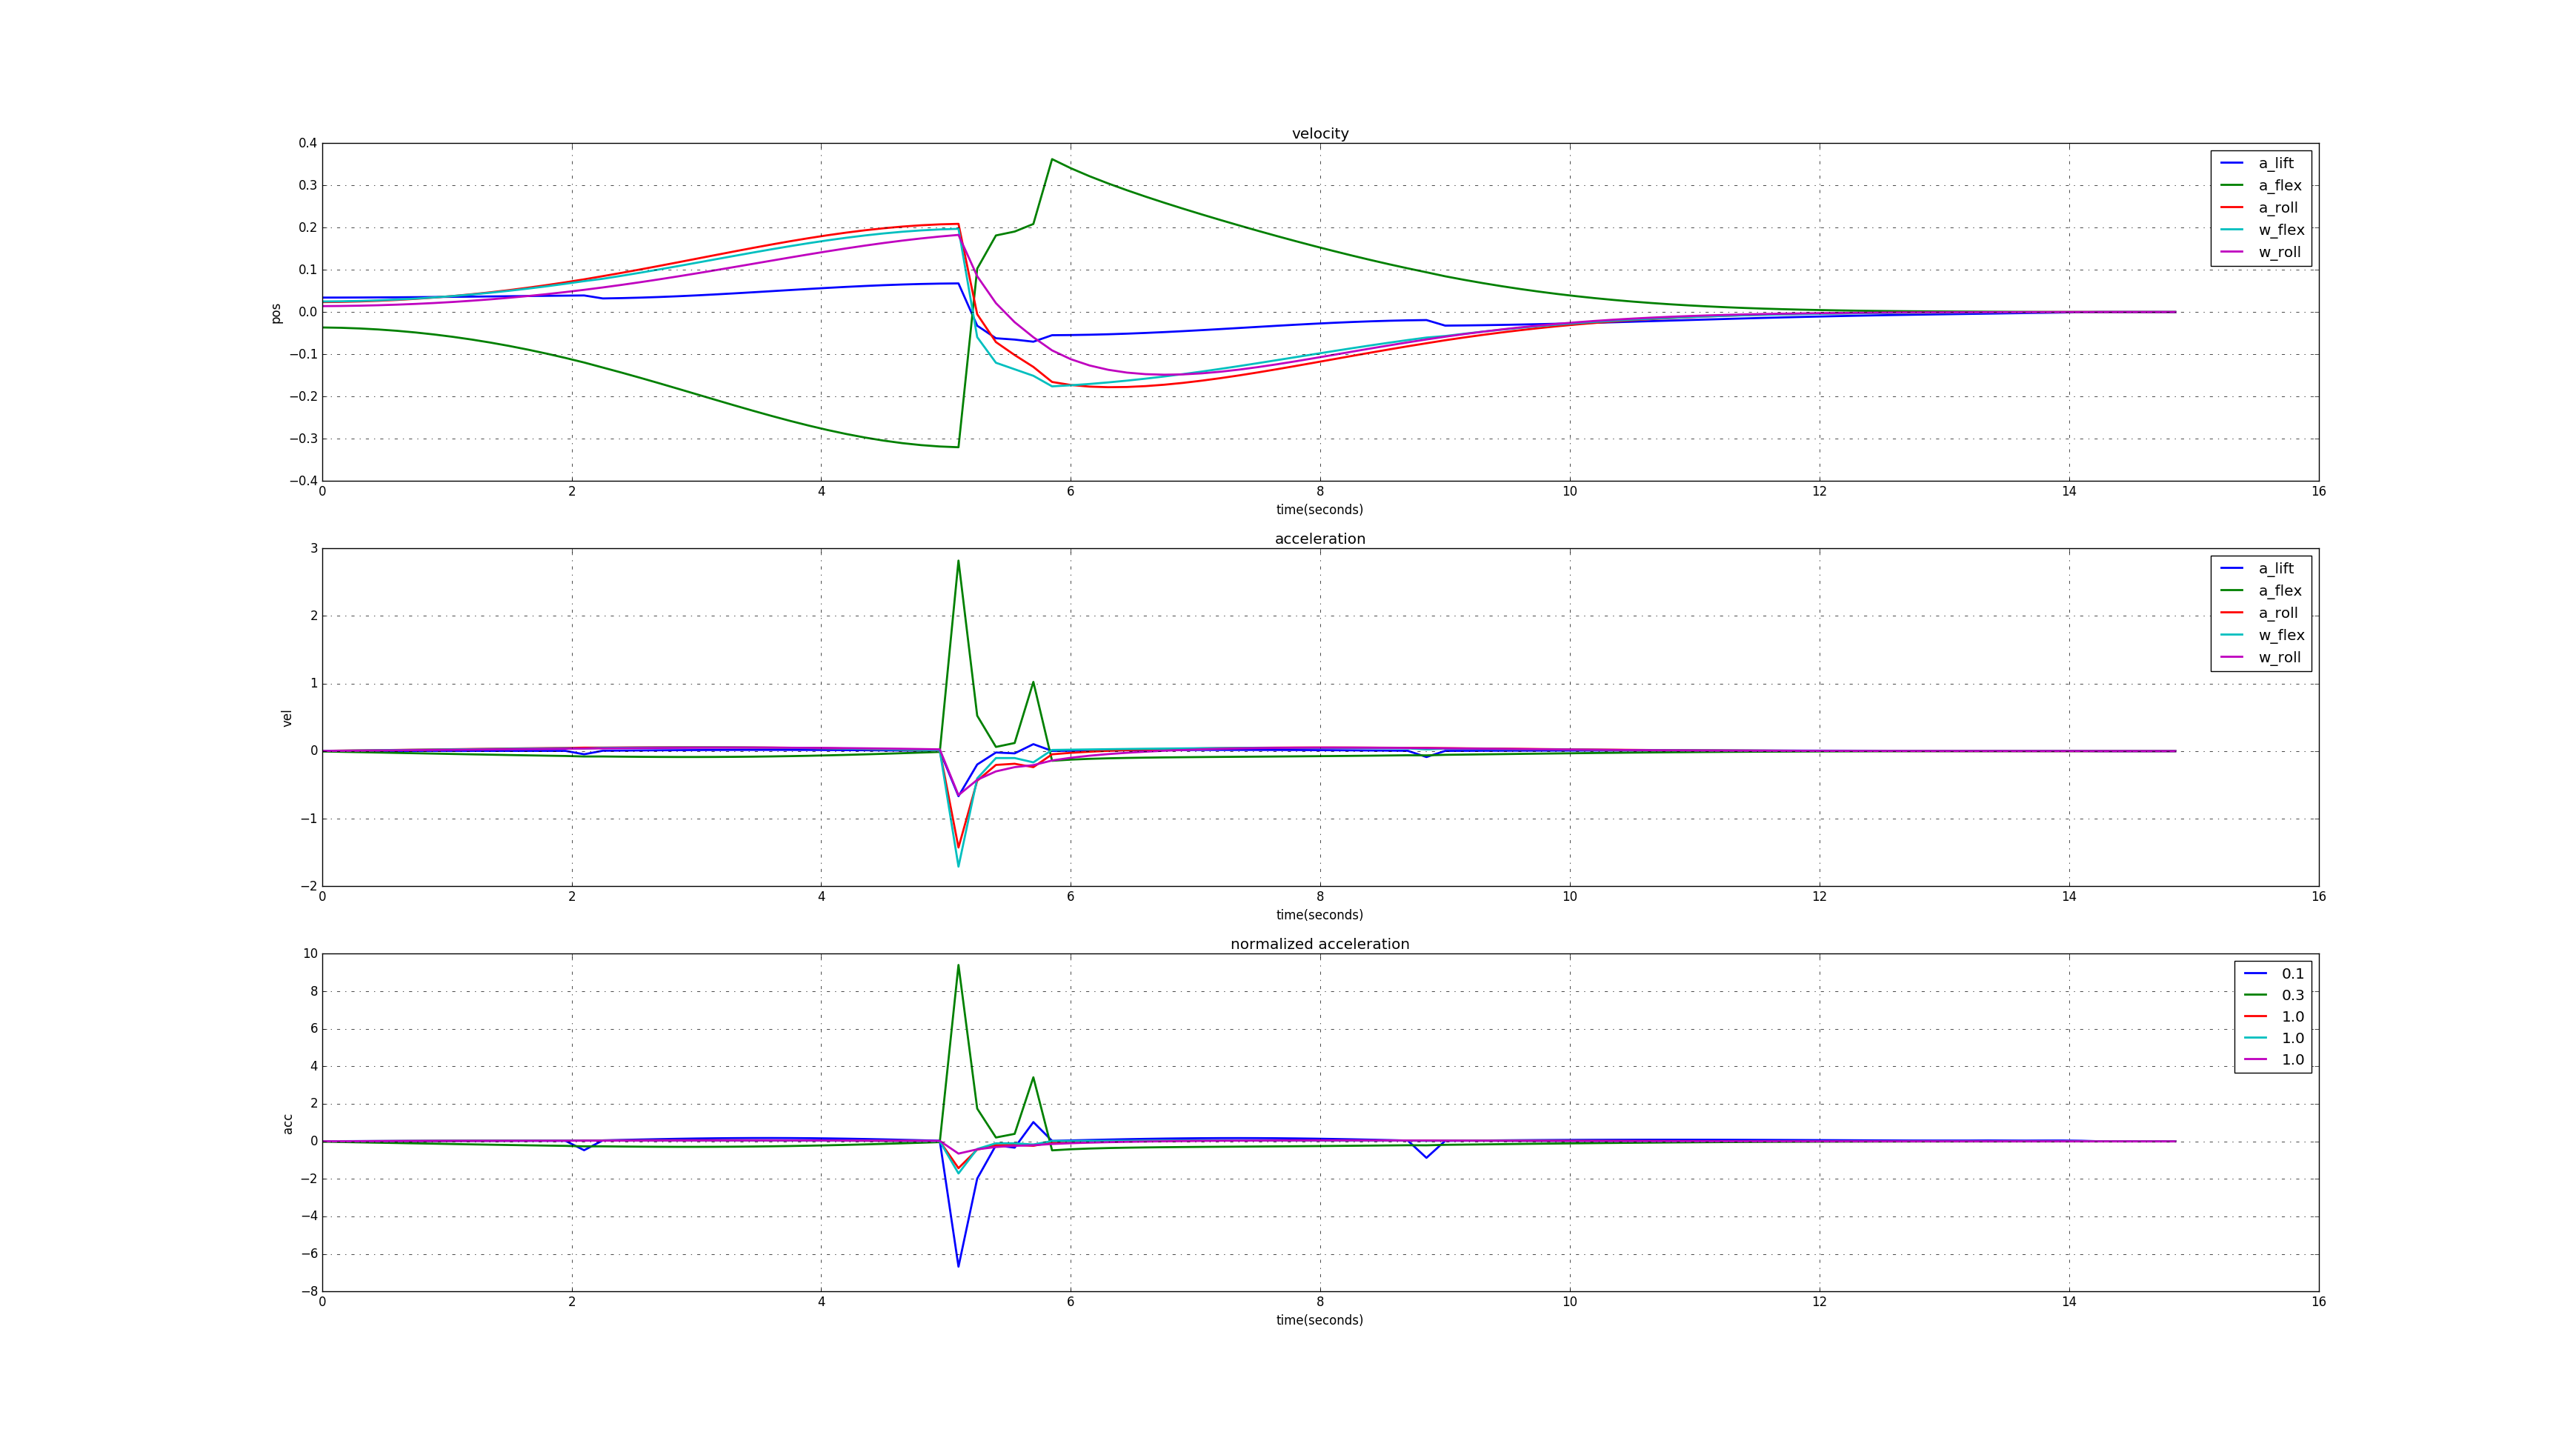
\includegraphics[width=\linewidth]{2020.05.17/ideal_acc_9_6.png}
            \label{fig:accelerations_ideal}
            \caption{(Top): Desired velocity values from \cref{fig:idealVel}. (Middle): Desired acceleration values calculated by taking the difference between adjacent velocity points and dividing by the time step. (Bottom): Desired joint acceleration values normalized by acceleration limits, displayed in the legend.} 
        \end{figure}   
        \begin{figure}
            \centering
            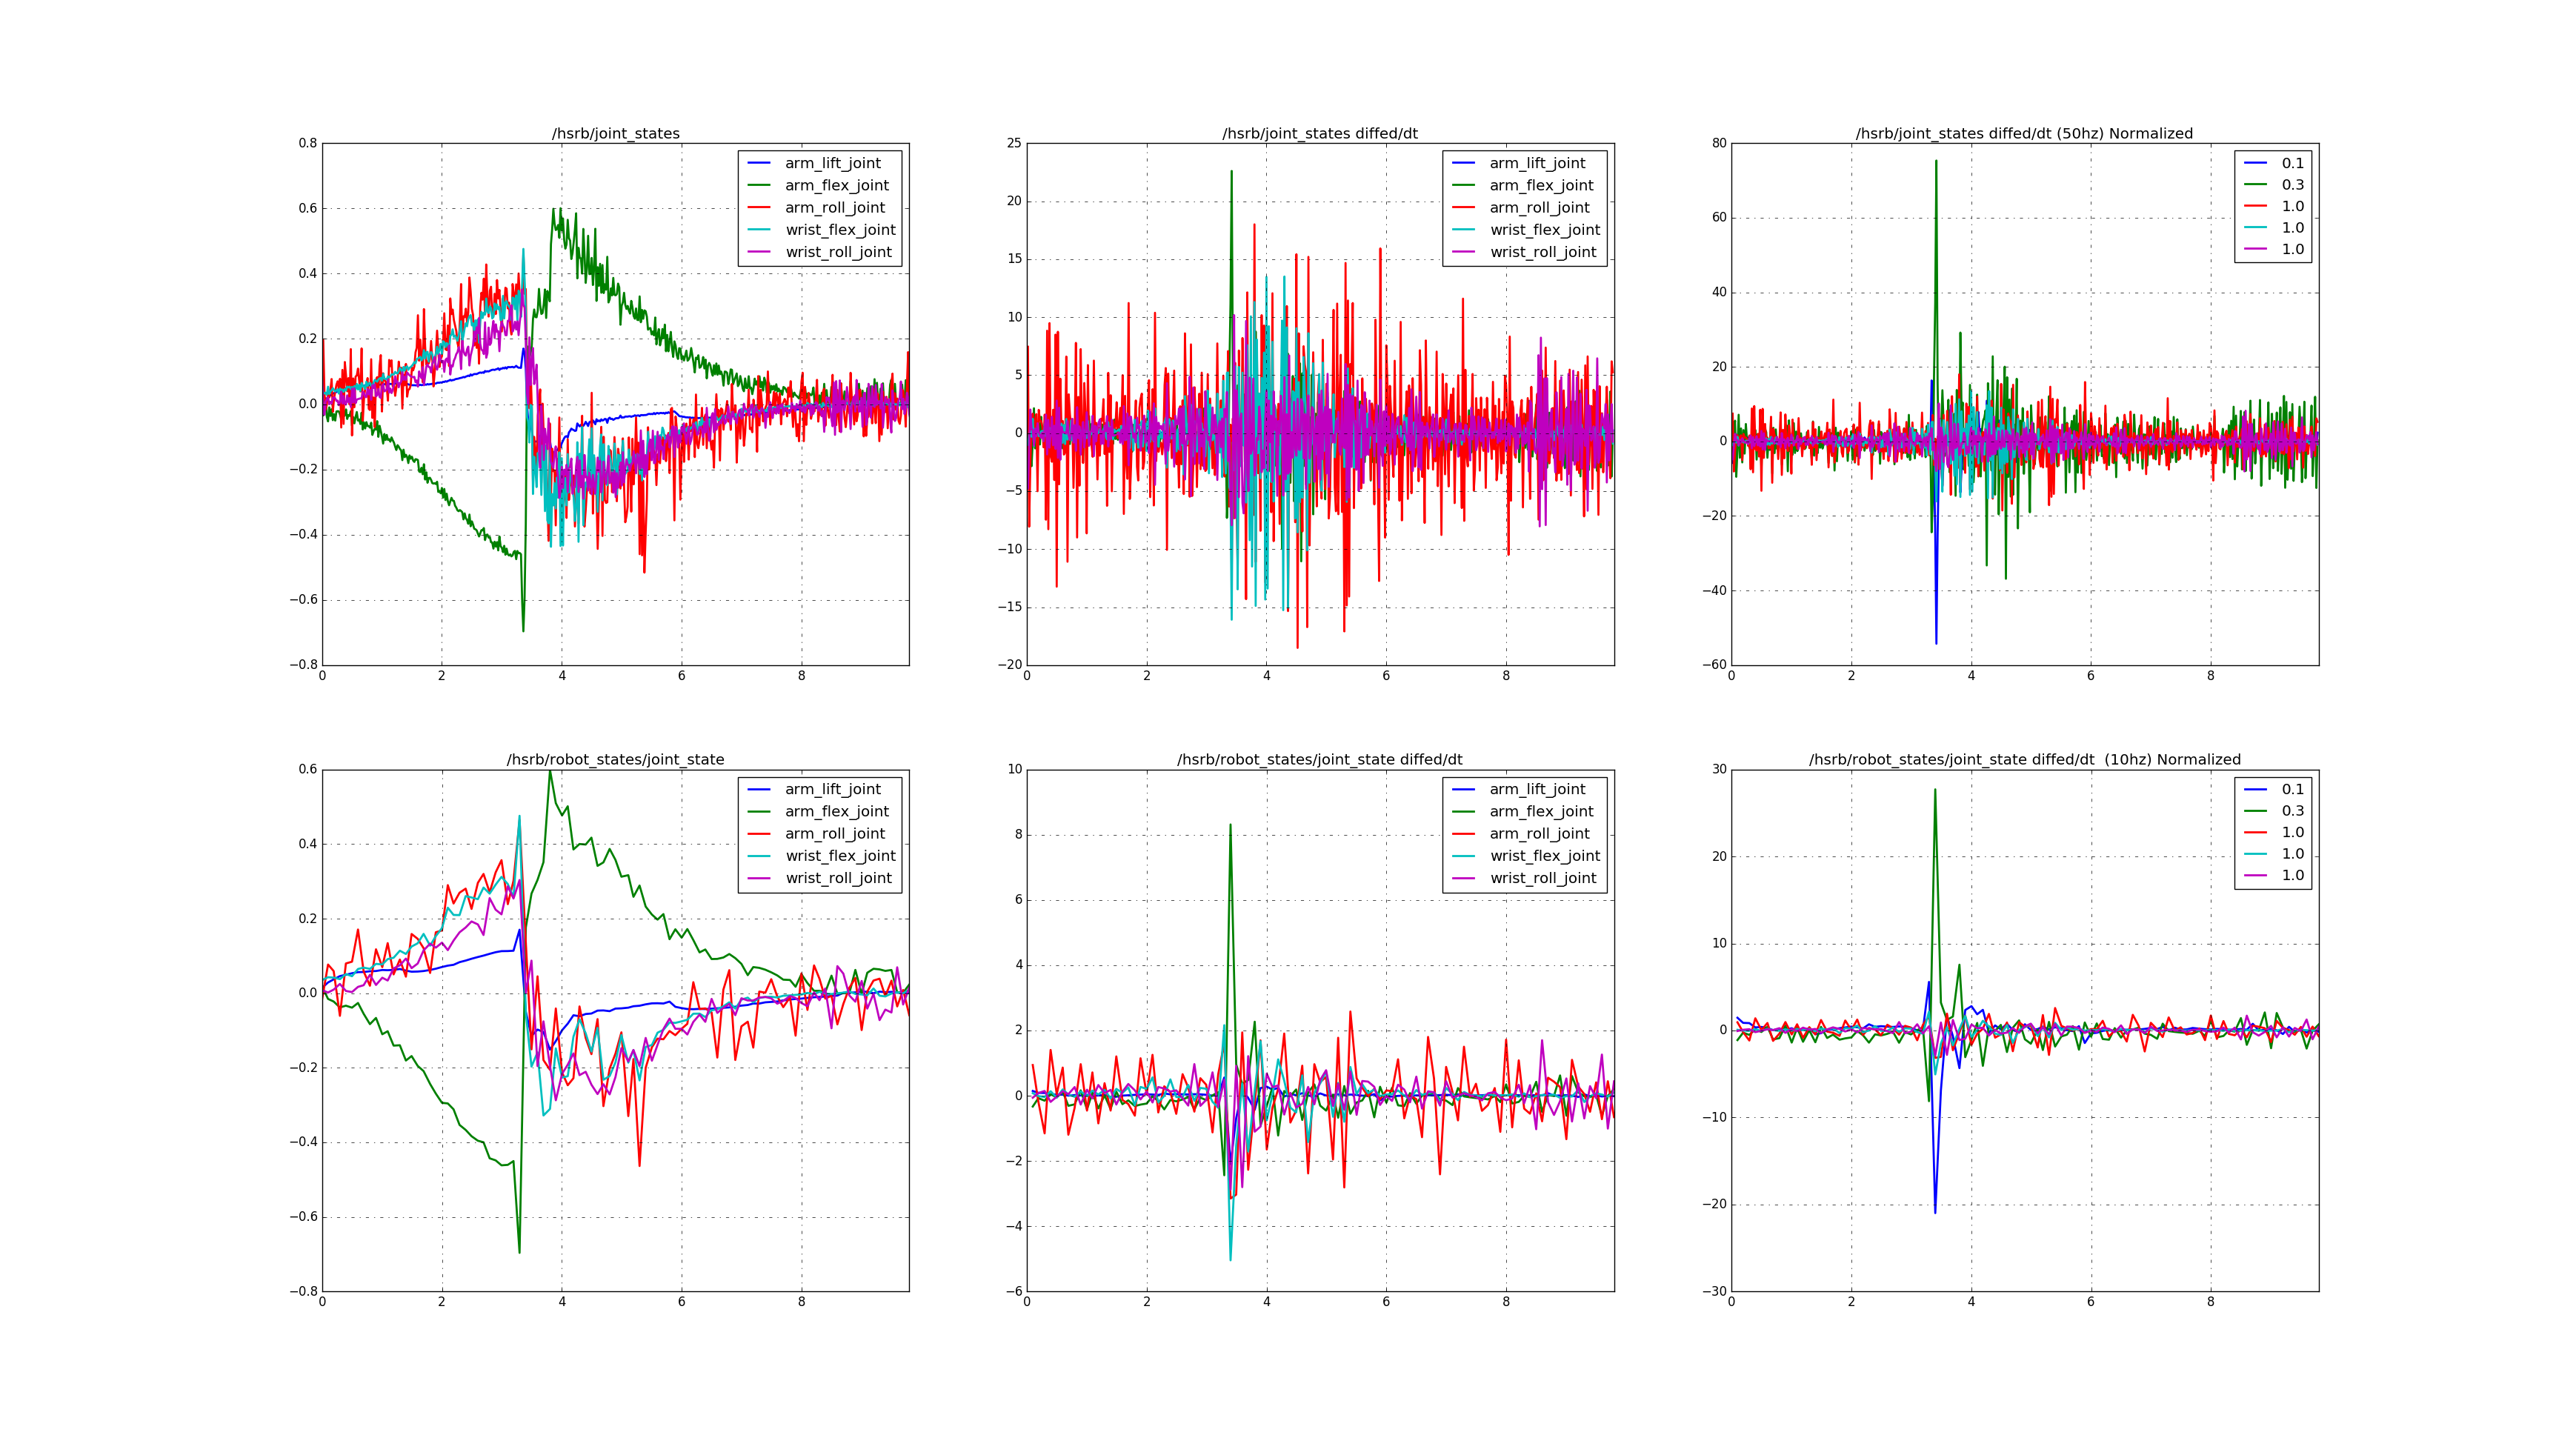
\includegraphics[width=\linewidth]{2020.05.17/accelerations_adjusted.png}
            \label{fig:accelerations_diffed}
            \caption{
                HSR arm joint accelerations obtained by taking the differentiating velocity with respect to the timestep. (Top row): data from /hsrb/joint-states ROS topic, which receives data from Gazebo at 50 Hz. (Bottom row): data from hsrb/robot-states/joint-state, which subsamples the data from /hsrb/joint-states through the HSR joint-state-publisher at 10 Hz. (First column): Velocity published from the respective topics. (Second column): Acceleration values calculated by taking the difference between adjacent velocity points and dividing by the time step. (Third column): Joint acceleration values normalized by acceleration limits, displayed in the legend.} 
        \end{figure}
        
        % \subsubsection{Joint Effort?}
        %     The plot of joint effort in \cref{fig:effjoints} shows that the base joints are nearing the effort limits of ~11. On the one hand, it is approaching the effort limit, but is applying maximum effort good and expected behavior?

    \newpage     
    \section{Conclusion}
        This paper introduces the drive-by pick-and-place method and implements it on the Toyota HSR to accomplish the pick-and-place task in a simplified environment. It is demonstrated that the whole-body drive-by planning method implemented on the HSR succeeds in accomplishing the pick-and-place task and generates trajectories that are smooth in position through the use of AICO for planning an extended grasping phase.
        \par This method in its current implementation has certain limitations. The trajectory has not yet been executed on the physical HSR, so differences in the magnitude of noise on joint measurements and measured joint accelerations may differ from the values in simulation.

        \par The predefined drive-by base trajectory is linear and assumed to be given prior to planning. Moreover, the start time and duration of the sub-grasping phase of the grasping step is pre-specified. This results in the HSR having to drive to a designated start pose to begin the grasping phase and assumes that a 1.4-meter path parallel to the table edge is collision-free. Further work would incorporate an additional path planning step to identify a base trajectory for the grasping step that is collision-free and brings the robot sufficiently close to the grasping target for the duration necessary to grasp the object. Identifying the earliest base pose that is within reaching distance to the target object could aid in determining the optimal start time for the sub-grasping step.

        \par This project only plans for grasping a soda can. The HSR gripper is capable of grasping larger objects, so gripping duration and the distance to separate gripper fingers should also be parameters for the algorithm to determine.

        \par The soda can was placed near the edge of the table since the HSR has poor reachability. Further work on adjusting the height of the table and the distance from the edge of the table to place the soda can is recommended to aid in identifying valid grasping scenarios.

        \par Using fiducial markers allows objects to be easily identified using computer vision. The HSR has an Nvidia Jetson TK1 installed as an auxiliary computer to enable GPU computing. This allows the HSR to perform objection recognition using neural networks with algorithms such as YOLO. Running YOLO and training new models on the HSR is outlined in the HSR documentation. \cite{noauthor_hsrb_manual_nodate}.

        \par The HSR is asymetrical, with the arm flex joint left of the centerline of the torso (\cref{fig:arm-flex-joint}), so the grasping motion differs depending on which side of the HSR the soda can located. For this project, trajectories were analyzed for a scenario where HSR drove by a table such that the table and soda can were located on the right side of the HSR. It may be necessary to define a new set of taskmap costs and activation timings for the case where the soda can is on the left side of the HSR during a drive-by base trajectory. Different distances between the HSR and the table may be tested, for target objects on both sides, to determine the optimal distances at which to perform the grasping task. It may be of interest to investigate the possibility of rotating the HSR base 180 degrees when the soda can is on the left side and driving the HSR omnibase backwards along the base trajectory. Then, the soda can can be positioned on the right side of the HSR for any given drive-by base trajectory.

        \par This project plans motion in a static environment. However, EXOTica allows for planning in a dynamic environment as demonstrated in \cite{yang_planning_2018}. Extending the method to a time-varying environment would increase the HSR's utility as a service robot for human interaction in real-world scenarios.

        %     \par 
        %     [Recap of method ]
        %     [Putting it all together: Insert section with whole motion plan.]
        % subsection{Extensions}
        %     \begin{itemize}
        %         \item Currently requires a predetermined trajectory. Can find one itself
        %         \item Currently, timing of grasps is hard coded since the HSR positions itself relative to the table and soda can. The relative positioning assumes open space surrounding the table.
        %         \item Include moving obstacles
        %         \item Use object detection/recognition instead of apriltags. HSR has some surface detection and can use YOLO with the nvidia jetson TK1.
        %         \item self identify optimal time step
        %     \end{itemize}
    \newpage
\iffalse TEXT \cite{lavalle_rapidly-exploring_1998} \fi
\section{Bibliography}
    \bibliography{references}
\section{Appendix}
    \subsection{Risk Assessment}
        \includepdf[pages={1,2}]{RiskAssessmentSigned_all}
    
\end{document}
    % \begin{itemize}
    %     \item Project title: RoboCup@ Home: motion planning for mobile robot navigation. Include Robocup@ home competition description as a motivation for the project.
    %     \item Overview of the problem at hand: drive-by pick and place problem with the Toyota HSR Robot. Include a brief description of the HSR and tech specs/features. General problem overview of picking up a cylindrical object from a table.
    %     \item Project description (these are from the project description on the 4yp website from early 2019. The project Ioannis shared with me at the start of the academic year revolved more specifically around the drive-by pick-and-place problem and implementing the RRTConnect, AICO combination detailed in the Pick-and-Place planning in time-configuration space paper)
    %     \begin{itemize}
    %         \item Easily Attainable: A focused literature survey on search-based and sampling-based planning, and optimal control. Plan paths for the HSR robot in a given arena. Avoid collisions and optimise for time taken to reach goal. Integrate sensory information and update internal representations of the environment. Guide a person to reach a goal location. (This can be done with the hsr interface/navigation stack)
    %         \item Medium Complexity: Dynamically changing environments. Navigate around people and deal with dynamic obstacle
    %         changes. Extensive evaluation in simulation and first tests on the real robot platform. (Haven't done extensive evaluation, but there is the capacity to send obstacle trajectories to the planning scene for the AICO solver in exotica)
    %         \item Advanced: Plan paths through variable configuration spaces, e.g. a path can be made accessible by pushing a chair aside.
    %         Evaluate on the real system. (Have not accomplished yet.)
    %     \end{itemize}
    %     \item Main point: Solving a time-indexed, drive-by pick and place problem by optimising a whole body trajectory (to address reachability issues).
    % \end{itemize}



%     \section{Literature Review 10-15 pages}
%     \begin{itemize}
%         \item RRTConnect(2-3 pages)
%         \item AICO solver (2-3 pages)
%         \item Planning in Time-Configuration Space for Efficient Pick-and-Place in Non-Static Environments with Temporal Constraints (3-5 pages)
%         \item maybe include: Apriltag visual fiducial system (1-2 pages)
%     \end{itemize}
% \section{Related Work}
%     \subsection{RRTConnect}
        

% \section{Technical (15-20 pages)}
%     \begin{itemize}
%         \item Preliminary work.
%         \begin{itemize}
%             \item General overview of ROS framework.
%             \item Relevant hardware/features of the HSR: Sensors and joints, type of end effector. ROS-based software, navigation stack, trajectory controllers.
%         \end{itemize}
%         \item Description of problem
%         \begin{itemize}
%             \item wrs competition gazebo world with tables, shelf, and two people. Drive-by-pick up a mug/bottle on table and place on a shelf. The complicated part is the drive-by pickup. Getting to the start pose of the pickup trajectory and getting to/placing the object can be done with the hsr interface. I have it mostly in place. Need to make it work in the wrs world which shouldn't take too much extra time. 
%             \item Introduce bare bones empty world setup for testing with ikea nyboda table and soda can. Ikea Nyboda table is used since it is the model of table available in the area of testing (ori big meeting room). A soda can is used because it is a default gazebo tutorial asset for the hsr.
%         \end{itemize}
%         \item Approaches
%         \begin{itemize}
%             \item Whole body planning with the AICO solver.
%             \item assumptions and required information/sensor data:
%             \begin{itemize}
%                 \item planning scene with object (table and bottle) locations and collision geometry known /obtainable.
%                 \item trajectory of base / start and end points of trajectory known/obtainable.
%                 \item Duration of base trajectory does not violiate hsr velocity constraints.
%                 \item HSR python interface to move to the starting position, using cameras and depth camera. Map server for wrs world.
%                 \item There is the option to include the trajectory and geometry of obstacles for time-indexed planning.
%             \end{itemize}
%             \item constraints, costs, timing of constraints (grasping and axis-alignment) and problem engineering. Justification and explanation of hand-tuned costs.
%             \item analysis of output trajectories. position, velocity, acceleration. material from emails. Smoothness, noise, sampling rates and possible interpolation.
%             \item (if time permits/need more pages) demonstrate/quantify the height of table and distance from table edge of bottle the hsr can reach. (plot of table height and bottle distance vs success of grasping?)
%             \item Could/should I compare the output trajectory of the whole body AICO problem with the rrtconnect and snopt/ik. Noting the reachability issue could justify the deviation from the method outlined in the pick-and-place in time-configuration space paper. I could graph the trajectory output using scripts I wrote already.
%         \end{itemize}
%         \item (if time permits and if there is space) Put it all together in the wrs world and demonstrate feasibility. Nearly there. Have april tags working in gazebo. Probably need to hard code the location of placement though. Will try to get it working in the wrs world.
%     \end{itemize}
% \section{Conclusion 2-3 pages}
% \begin{itemize}
%     \item Recap whole body planning for pick and place problem.
%     \item Possible extensions/future directions. Point back to assumptions and required information input.
% \end{itemize}
% \section{References ~2-3 pages}
% \section{Appendices ~3-5 pages}
% \begin{itemize}
%     \item Appendices content counts towards page count.
%     \item Code
%     \item Images and maps of world/experimental setup.
% \end{itemize}